\documentclass[12pt,a4paper]{report}

% ================== PACKAGE CƠ BẢN ==================
\usepackage[utf8]{inputenc}
\usepackage[T5]{fontenc}
\usepackage[vietnamese]{babel}
\usepackage{graphicx}
\usepackage{geometry}
\usepackage{tikz}
\usepackage{setspace}
\usepackage{tocloft}
\usepackage{titlesec}
\usepackage[hypertexnames=false]{hyperref}
\usepackage{array}
\usepackage{float}
\usepackage{ragged2e}
\usepackage{indentfirst}
\usepackage{enumitem}
\usepackage{placeins}

% ================== CĂN LỀ ==================
\geometry{
    top=2cm,
    bottom=2cm,
    left=2cm,
    right=2cm
}

% ================== CẤU HÌNH TIẾNG VIỆT ==================
\addto\captionsvietnamese{
    \renewcommand{\contentsname}{Mục lục}
    \renewcommand{\listfigurename}{Danh sách hình vẽ}
    \renewcommand{\listtablename}{Danh sách bảng}
    \renewcommand{\figurename}{Hình}
    \renewcommand{\tablename}{Bảng}
}

% ================== LINK TRONG PDF ==================
\hypersetup{
    colorlinks=false,
    pdfborder={0 0 0}
}

% ================== ĐỘ SÂU ĐÁNH SỐ VÀ MỤC LỤC ==================
\setcounter{tocdepth}{3}
\setcounter{secnumdepth}{3}

% ================== FORMAT CHƯƠNG TRONG NỘI DUNG ==================
\titleformat{\chapter}[display]
{\bfseries\Huge}
{Chương \thechapter.}
{0.4cm}
{}
    
\titlespacing*{\chapter}
{0pt}
{1cm}
{2cm}

% ================== FORMAT MỤC LỤC GIỐNG MẪU ==================

% Tiêu đề mục lục
\renewcommand{\cfttoctitlefont}{\LARGE\bfseries}
\renewcommand{\cftaftertoctitle}{\vspace{1cm}}

% Hiển thị chương dạng: Chương 1. Giới thiệu
\renewcommand{\cftchappresnum}{Chương~}
\renewcommand{\cftchapaftersnum}{.~}
\setlength{\cftchapnumwidth}{2.6cm}

% Dấu chấm dẫn trang
\renewcommand{\cftchapleader}{\cftdotfill{\cftdotsep}}
\renewcommand{\cftsecleader}{\cftdotfill{\cftdotsep}}
\renewcommand{\cftsubsecleader}{\cftdotfill{\cftdotsep}}

% Font trong mục lục
\renewcommand{\cftchapfont}{\normalsize\bfseries}
\renewcommand{\cftchappagefont}{\normalsize\bfseries}
\renewcommand{\cftsecfont}{\normalsize}
\renewcommand{\cftsecpagefont}{\normalsize}
\renewcommand{\cftsubsecfont}{\normalsize}
\renewcommand{\cftsubsecpagefont}{\normalsize}

% Khoảng cách dòng trong mục lục
\setlength{\cftbeforechapskip}{0.25cm}
\setlength{\cftbeforesecskip}{0.08cm}
\setlength{\cftbeforesubsecskip}{0.05cm}

% Căn lề các cấp mục lục
\setlength{\cftchapindent}{0cm}
\setlength{\cftsecindent}{0.65cm}
\setlength{\cftsubsecindent}{1.25cm}

% Độ rộng phần số thứ tự
\setlength{\cftsecnumwidth}{1.1cm}
\setlength{\cftsubsecnumwidth}{1.4cm}

% ================== FORMAT DANH SÁCH HÌNH VẼ, BẢNG ==================
\renewcommand{\cftloftitlefont}{\Large\bfseries}
\renewcommand{\cftlottitlefont}{\Large\bfseries}

\renewcommand{\cftfigleader}{\cftdotfill{\cftdotsep}}
\renewcommand{\cfttableader}{\cftdotfill{\cftdotsep}}

\setlength{\cftbeforefigskip}{0.08cm}
\setlength{\cftbeforetabskip}{0.08cm}

% ================== LỆNH KẺ VIỀN TRANG BÌA ==================
\newcommand{\drawcoverborder}{
\begin{tikzpicture}[remember picture, overlay]
    % Viền ngoài
    \draw[line width=1.4pt]
        ([xshift=1.35cm,yshift=-1.35cm]current page.north west)
        rectangle
        ([xshift=-1.35cm,yshift=1.35cm]current page.south east);

    % Viền trong
    \draw[line width=0.6pt]
        ([xshift=1.55cm,yshift=-1.55cm]current page.north west)
        rectangle
        ([xshift=-1.55cm,yshift=1.55cm]current page.south east);
\end{tikzpicture}
}

\begin{document}

\justifying
\setstretch{1.3}
\setlength{\parindent}{1.25cm}
\setlength{\parskip}{0pt}

% ========================= TRANG BÌA 1 =========================
\begin{titlepage}

\drawcoverborder

\centering
\setstretch{1.25}

{\large\bfseries ĐẠI HỌC QUỐC GIA HÀ NỘI\par}
\vspace{0.25cm}
{\large\bfseries TRƯỜNG ĐẠI HỌC CÔNG NGHỆ\par}

\vspace{0.9cm}


\includegraphics[width=6cm]{logo.png}

\vspace{0.7cm}

{\large\bfseries Nhóm ĐT1.N11\par}
\vspace{0.25cm}

{\large\bfseries Thành viên: 23020074 - Bùi Thái Học\par}
\vspace{0.08cm}
{\large\bfseries 21020301 - Đào Ngọc Hải Đăng\par}
\vspace{0.08cm}
{\large\bfseries 23020105 - Vũ Quốc Long\par}
\vspace{0.08cm}
{\large\bfseries 23020157 - Trần Thị Phương Thảo\par}

\vspace{1.6cm}

{\LARGE\bfseries CAMPUS CYCLE PLATFORM\par}

\vspace{1.7cm}

{\Large\bfseries BÁO CÁO BÀI TẬP\par}

\vspace{0.5cm}

{\large\bfseries Môn học: Phân tích và thiết kế các hệ thống thông tin\par}

\vfill

{\large\bfseries HÀ NỘI -- 2026\par}

\end{titlepage}

% ========================= TRANG BÌA 2 =========================
\begin{titlepage}

\drawcoverborder

\centering
\setstretch{1.3}

{\large\bfseries ĐẠI HỌC QUỐC GIA HÀ NỘI\par}
\vspace{0.3cm}
{\large\bfseries TRƯỜNG ĐẠI HỌC CÔNG NGHỆ\par}

\vspace{2.3cm}

{\large\bfseries Nhóm ĐT1.N11\par}
\vspace{0.3cm}

{\large\bfseries Thành viên: 23020074 - Bùi Thái Học\par}
\vspace{0.1cm}
{\large\bfseries 21020301 - Đào Ngọc Hải Đăng\par}
\vspace{0.1cm}
{\large\bfseries 23020105 - Vũ Quốc Long\par}
\vspace{0.1cm}
{\large\bfseries 23020157 - Trần Thị Phương Thảo\par}

\vspace{1.8cm}

{\LARGE\bfseries CAMPUS CYCLE PLATFORM\par}

\vspace{2cm}

{\Large\bfseries BÁO CÁO BÀI TẬP\par}

\vspace{0.5cm}

{\large\bfseries Môn học: Phân tích và thiết kế các hệ thống thông tin\par}

\vspace{2.1cm}

{\large\bfseries Cán bộ hướng dẫn: TS. Dư Phương Hạnh\par}

\vfill

{\large\bfseries HÀ NỘI -- 2026\par}

\end{titlepage}

% ========================= MỤC LỤC =========================
\pagenumbering{roman}

\tableofcontents
\clearpage

\listoffigures
\clearpage

\listoftables
\clearpage

\pagenumbering{arabic}

% ========================= NỘI DUNG =========================

\chapter{Giới thiệu}

\section{Bối cảnh đề tài}

Trong môi trường các trường tư thục tự chủ tài chính, nhu cầu sử dụng và
thay đổi đồ dùng học tập, đồng phục, sách giáo khoa, thiết bị điện tử và các vật
dụng cá nhân diễn ra thường xuyên theo từng năm học hoặc học kỳ. Điều này dẫn
đến việc nhiều vật phẩm vẫn còn giá trị sử dụng nhưng không còn phù hợp với
nhu cầu của chủ sở hữu. Song song với đó, các hoạt động thiện nguyện, gây quỹ và
quyên góp trong nhà trường ngày càng được quan tâm nhằm xây dựng môi trường
học tập gắn kết và hỗ trợ cộng đồng. Tuy nhiên, phần lớn các hoạt động này hiện
vẫn được triển khai theo phương thức truyền thống, thiếu nền tảng quản lý tập
trung và chưa tận dụng được nguồn tài nguyên còn dư thừa trong nội bộ trường
học. Từ thực tế trên, việc xây dựng một hệ thống hỗ trợ thanh lý và
quyên góp đồ cũ trong phạm vi trường học là cần thiết nhằm nâng cao hiệu quả
sử dụng tài nguyên, tăng cường kết nối cộng đồng và hỗ trợ các hoạt động thiện
nguyện.

\section{Xác định bài toán}

Bài toán đặt ra là xây dựng một hệ thống cho phép học sinh, giáo viên và
các thành viên trong trường học có thể mua bán hoặc quyên góp các vật phẩm cũ
còn giá trị sử dụng trong một môi trường nội bộ an toàn và minh bạch. Hệ thống
cần hỗ trợ các hoạt động chính như đăng tải sản phẩm, kiểm duyệt nội dung, tìm
kiếm vật phẩm, tham gia chiến dịch gây quỹ, quyên góp vật phẩm, quản lý giao
dịch và thống kê hoạt động. Đồng thời, hệ thống phải đảm bảo tính bảo mật, tính
minh bạch trong giao dịch và khả năng mở rộng trong tương lai.

\section{Các vấn đề hiện tại và giải pháp liên quan}

\subsection{Lãng phí tài nguyên}

Trong môi trường học đường, vòng đời sử dụng của nhiều loại vật phẩm như
sách giáo khoa, đồng phục, thiết bị học tập hoặc dụng cụ câu lạc bộ thường khá
ngắn do sự thay đổi theo năm học hoặc nhu cầu cá nhân. Điều này dẫn đến việc nhiều vật phẩm vẫn còn giá trị sử dụng nhưng không còn được dùng đến và bị bỏ
không hoặc thải bỏ. Thực trạng này gây ra sự lãng phí đáng kể về mặt kinh tế,
đồng thời tạo áp lực đối với môi trường do làm gia tăng lượng rác thải không cần
thiết. Hiện nay, việc tái sử dụng các vật phẩm này chủ yếu được thực hiện thông
qua trao đổi trực tiếp giữa học sinh và giáo viên, các nhóm mạng xã hội nội bộ
hoặc các hoạt động quyên góp được tổ chức theo từng đợt. Tuy nhiên, các giải
pháp này vẫn còn nhiều hạn chế như khó tiếp cận đúng người có nhu cầu, thiếu cơ
chế quản lý tập trung và chưa tạo được khả năng theo dõi, thống kê hiệu quả sử
dụng tài nguyên. Do đó, tỷ lệ tái sử dụng vật phẩm trong môi trường học đường
vẫn còn thấp.

\subsection{Hoạt động quyên góp và gây quỹ còn rời rạc}

Các hoạt động quyên góp và gây quỹ trong trường học hiện nay thường được
triển khai theo từng chiến dịch ngắn hạn do nhà trường, câu lạc bộ hoặc các tổ
chức phát động. Tuy nhiên, chưa tồn tại một nền tảng hỗ trợ kết nối liên tục giữa
người muốn đóng góp và các chiến dịch đang cần hỗ trợ, khiến các hoạt động này
mang tính thời điểm và khó duy trì lâu dài. Để triển khai các hoạt động quyên
góp, nhiều đơn vị hiện sử dụng các công cụ như biểu mẫu trực tuyến, bảng tính
hoặc các kênh thông báo nội bộ. Mặc dù những công cụ này giúp triển khai nhanh,
chúng lại khiến dữ liệu bị phân tán, khó theo dõi số lượng vật phẩm hoặc khoản
đóng góp nhận được. Ngoài ra, quá trình thống kê thủ công còn làm giảm tính
minh bạch và tăng nguy cơ sai sót trong quá trình quản lý.

\subsection{Thiếu nền tảng giao dịch nội bộ đáng tin cậy}

Hoạt động trao đổi và mua bán vật phẩm trong môi trường học đường hiện
chủ yếu được thực hiện thông qua các nền tảng mạng xã hội hoặc giao dịch trực
tiếp. Các nền tảng như Facebook Marketplace, nhóm Facebook nội bộ, Zalo hoặc
các sàn thương mại điện tử thường được sử dụng để kết nối người bán và người
mua. Tuy nhiên, các giải pháp này chưa thực sự phù hợp với môi trường trường
học do không có cơ chế xác thực thành viên nội bộ, thiếu quy trình kiểm duyệt
nội dung và chưa hỗ trợ phân loại sản phẩm theo nhu cầu đặc thù của nhà trường.
Điều này dẫn đến rủi ro về an toàn giao dịch, tranh chấp giữa các bên và làm giảm
mức độ tin cậy của hệ thống.

\subsection{Công tác quản lý chiến dịch còn thủ công}

Hiện nay, việc quản lý các chiến dịch gây quỹ và quyên góp phần lớn vẫn được
thực hiện thủ công thông qua bảng tính, biểu mẫu hoặc các phương thức quản lý giấy tờ truyền thống. Những công cụ như Microsoft Excel, Google Sheets hoặc việc
tổng hợp dữ liệu qua tin nhắn thường được sử dụng để lưu trữ và quản lý thông
tin. Phương pháp quản lý này gặp nhiều hạn chế khi quy mô chiến dịch tăng lên,
do dữ liệu dễ phân tán, khó kiểm soát và dễ phát sinh sai sót trong quá trình nhập
liệu. Đồng thời, việc tổng hợp báo cáo và thống kê thường tốn nhiều thời gian, yêu
cầu nhiều nhân lực và làm giảm hiệu quả quản lý chung của chiến dịch.

\subsection{Nhu cầu xây dựng hệ thống mới}

Từ các hạn chế của các giải pháp hiện tại, cần xây dựng một hệ thống tập
trung nhằm giải quyết các vấn đề còn tồn tại và nâng cao hiệu quả quản lý. Hệ
thống cần đáp ứng các mục tiêu sau:

\begin{itemize}[label=--, leftmargin=1.2cm]

\item Quản lý hoạt động mua bán và quyên góp theo mô hình tập trung.

\item Kiểm duyệt nội dung trước khi công khai nhằm đảm bảo tính phù hợp và an toàn.

\item Quản lý các chiến dịch gây quỹ một cách minh bạch và dễ theo dõi.

\item Hỗ trợ giao dịch an toàn giữa các thành viên trong hệ thống.

\item Nâng cao hiệu quả tái sử dụng tài nguyên trong môi trường trường học.

\end{itemize}


\section{Mục tiêu hệ thống}

Hệ thống quyên góp và thanh lý đồ cũ trong trường học được xây
dựng nhằm tạo ra một nền tảng nội bộ dành cho học sinh, giáo viên và các tổ chức
trong trường có thể mua bán hoặc quyên góp các vật phẩm còn giá trị sử
dụng. Hệ thống hướng tới việc giải quyết tình trạng lãng phí tài nguyên trong môi
trường học đường, đồng thời hỗ trợ các hoạt động thiện nguyện, gây quỹ và quyên
góp thông qua cơ chế quản lý tập trung và minh bạch. Ngoài ra, hệ thống còn giúp
chuẩn hóa quy trình kiểm duyệt nội dung, hỗ trợ quản lý giao dịch và tăng cường
mức độ an toàn khi thực hiện trao đổi giữa các thành viên trong trường. Các mục
tiêu chính của hệ thống được xây dựng nhằm giải quyết các vấn đề về 
quyên góp và tái sử dụng tài nguyên trong môi trường học đường. Cụ thể, hệ thống
hướng đến các mục tiêu sau:

\begin{itemize}[label=--, leftmargin=1.2cm]


\item Tạo môi trường mua bán và thanh lý đồ cũ an toàn trong phạm vi nội bộ trường học.

\item Hỗ trợ tổ chức, quản lý và theo dõi các hoạt động gây quỹ, quyên góp một cách hiệu quả.

\item Tăng cường khả năng tái sử dụng tài nguyên, góp phần giảm thiểu lãng phí và bảo vệ môi trường.

\item Cung cấp công cụ quản lý giao dịch, theo dõi hoạt động và thống kê dữ liệu hiệu quả.

\item Xây dựng cộng đồng học đường gắn kết, thúc đẩy tinh thần chia sẻ và hỗ trợ lẫn nhau.


\end{itemize}


\section{Phạm vi hệ thống}

Hệ thống được xây dựng để phục vụ các hoạt động mua bán, thanh
lý và quyên góp đồ cũ trong phạm vi các trường tư thục tự chủ tài chính. Phạm vi
chức năng của hệ thống được xác định nhằm giới hạn các chức năng sẽ được triển
khai trong giai đoạn phát triển và những chức năng không thuộc phạm vi xử lý
của hệ thống.

\subsection{Trong phạm vi hệ thống}

\begin{itemize}[label=--,leftmargin=1.2cm,itemsep=0.4em]
    \item Quản lý tài khoản người dùng
    \item Đăng tải, chỉnh sửa và quản lý bài đăng sản phẩm
    \item Kiểm duyệt sản phẩm và chiến dịch trước khi công khai
    \item Quản lý chiến dịch gây quỹ và quyên góp
    \item Hỗ trợ giao dịch mua bán sản phẩm
    \item Theo dõi và quản lý trạng thái vật phẩm quyên góp
    \item Quản lý báo cáo và thống kê quỹ chung
    \item Kết nối với hệ thống thanh toán trung gian
\end{itemize}

\subsection{Ngoài phạm vi hệ thống}

\begin{itemize}[label=--, leftmargin=1.2cm]

\item Không trực tiếp xử lý thanh toán hoặc lưu trữ thông tin ngân hàng của người dùng.

\item Không cung cấp dịch vụ vận chuyển hoặc giao nhận sản phẩm.

\item Không kiểm định chất lượng thực tế của sản phẩm được đăng tải.

\item Không giải quyết các tranh chấp phát sinh ngoài hệ thống.

\end{itemize}

\section{Tổng quan hệ thống}

Hệ thống được xây dựng như một nền tảng trực tuyến cho phép các thành
viên trong trường học tương tác với nhau thông qua hoạt động mua bán
và quyên góp vật phẩm. Bên cạnh việc hỗ trợ giao dịch sản phẩm, hệ thống còn
đóng vai trò hỗ trợ các chiến dịch thiện nguyện và gây quỹ do nhà trường hoặc
các tổ chức trong trường phát động. Toàn bộ quá trình đăng bài, tham gia chiến
dịch và giao dịch đều được quản lý tập trung nhằm tăng tính minh bạch và giảm
rủi ro.

\subsection{Ngữ cảnh hệ thống}

Hệ thống hoạt động như một nền tảng trung gian kết nối giữa người bán, người mua, người quyên góp, quản trị viên và các tổ chức trong trường học. Các tác nhân chính tương tác với hệ thống bao gồm những đối tượng sử dụng hoặc trao đổi dữ liệu với hệ thống trong quá trình vận hành. Mỗi tác nhân đảm nhận những vai trò và chức năng khác nhau nhằm đảm bảo hệ thống hoạt động hiệu quả.

\begin{itemize}[label=--, leftmargin=1.2cm]

\item \textbf{Thành viên (học sinh, giáo viên):} Thực hiện các hoạt động đăng tải sản phẩm, mua bán, quyên góp và tham gia các chiến dịch gây quỹ.

\item \textbf{Quản trị viên hệ thống:} Quản lý người dùng, kiểm duyệt nội dung, giám sát hoạt động hệ thống và xử lý các báo cáo phát sinh.

\item \textbf{Quản trị viên tổ chức:} Quản lý các chiến dịch gây quỹ, theo dõi vật phẩm quyên góp và thống kê hoạt động của tổ chức.

\item \textbf{Hệ thống thanh toán trung gian:} Tiếp nhận và xử lý thông tin thanh toán, đồng thời gửi kết quả giao dịch về hệ thống.

\end{itemize}

Người dùng thực hiện các hoạt động như đăng sản phẩm, tham gia chiến dịch, gửi yêu cầu mua hàng hoặc quyên góp thông qua hệ thống. Hệ thống tiếp nhận, xử lý, kiểm duyệt và lưu trữ dữ liệu phục vụ quản lý.

\subsection{Đặc điểm người dùng}

Hệ thống phục vụ nhiều nhóm người dùng khác nhau với nhu cầu sử dụng và quyền hạn riêng biệt. Mỗi nhóm người dùng sẽ tương tác với hệ thống theo vai trò và chức năng tương ứng.

\textbf{Thành viên (Member)}

Bao gồm học sinh và giáo viên trong phạm vi trường học. Đây là nhóm người dùng chính của hệ thống với các chức năng:

\begin{itemize}[label=--, leftmargin=1.2cm]
\item Đăng tải bài đăng sản phẩm.
\item Thực hiện mua bán, quyên góp.
\item Tham gia các chiến dịch gây quỹ.
\item Theo dõi giao dịch và trạng thái vật phẩm.
\end{itemize}

\textbf{Quản trị viên hệ thống (Administrator)}

Là nhóm người dùng chịu trách nhiệm quản lý và giám sát hoạt động của toàn bộ hệ thống, bao gồm:

\begin{itemize}[label=--, leftmargin=1.2cm]
\item Quản lý người dùng và nội dung hệ thống.
\item Kiểm duyệt sản phẩm và chiến dịch.
\item Theo dõi giao dịch và xử lý báo cáo.
\item Giám sát hoạt động chung của hệ thống.
\end{itemize}

\textbf{Quản trị viên tổ chức (Organization Administrator)}

Là đại diện của các tổ chức hoặc câu lạc bộ tham gia hệ thống với các nhiệm vụ:

\begin{itemize}[label=--, leftmargin=1.2cm]
\item Quản lý các chiến dịch thuộc tổ chức.
\item Theo dõi hoạt động gây quỹ và quyên góp.
\item Kiểm duyệt vật phẩm tham gia chiến dịch.
\item Tổng hợp và theo dõi kết quả chiến dịch.
\end{itemize}

\textbf{Hệ thống thanh toán (Billing System)}

Đây là hệ thống bên ngoài được tích hợp nhằm hỗ trợ xử lý giao dịch thanh toán:

\begin{itemize}[label=--, leftmargin=1.2cm]
\item Tiếp nhận thông tin thanh toán từ hệ thống.
\item Xử lý giao dịch trung gian.
\item Trả kết quả thanh toán về hệ thống chính.
\end{itemize}

\subsection{Mã nguồn hệ thống}

Để phục vụ cho công tác triển khai và đánh giá chất lượng phần mềm, toàn
bộ sản phẩm và mã nguồn của nền tảng CampusCycle được lưu trữ công khai trên
hệ thống quản lý mã nguồn GitHub.

Địa chỉ truy cập kho chứa (Repository) chính thức của dự án tại đường dẫn:

https://github.com/thaihoc1310/campus-cycle

\section{Kiến trúc công nghệ của hệ thống}

Campus Cycle được triển khai theo mô hình ứng dụng web nhiều lớp, trong đó
giao diện người dùng, tầng xử lý nghiệp vụ và tầng lưu trữ dữ liệu được tách
riêng để dễ phát triển, kiểm thử và mở rộng. Kiến trúc này phù hợp với đặc thù
của hệ thống vì các nhóm người dùng khác nhau như Thành viên, Quản trị viên
hệ thống và Quản trị viên tổ chức đều truy cập vào cùng một nền tảng nhưng sử
dụng các chức năng khác nhau.

\subsection{Mô hình kiến trúc tổng quát}

Hệ thống gồm ba lớp chính: lớp giao diện, lớp dịch vụ ứng dụng và lớp dữ
liệu. Lớp giao diện được xây dựng bằng React và chạy thông qua Vite. Người dùng
tương tác với hệ thống thông qua các trang như marketplace, chi tiết sản phẩm,
quản lý chiến dịch, dashboard quản trị và dashboard tổ chức. Các thao tác từ giao
diện được gửi tới backend thông qua các API dạng REST.

Lớp dịch vụ ứng dụng được xây dựng bằng FastAPI. Backend chịu trách nhiệm
tiếp nhận yêu cầu từ frontend, kiểm tra quyền truy cập, xử lý nghiệp vụ và trả dữ
liệu về cho giao diện. Các nhóm API được tổ chức thành nhiều router riêng như
xác thực tài khoản, người dùng, tổ chức, danh mục, vật phẩm, chiến dịch, giao
dịch, dashboard, chức năng dành cho thành viên và chức năng dành cho quản trị
viên tổ chức. Cách tổ chức này giúp mã nguồn dễ bảo trì và phản ánh rõ các phân
hệ nghiệp vụ của Campus Cycle.

Lớp dữ liệu sử dụng PostgreSQL 16 làm hệ quản trị cơ sở dữ liệu quan hệ.
Backend truy cập cơ sở dữ liệu thông qua SQLAlchemy ORM, còn Alembic được sử
dụng để quản lý lịch sử thay đổi lược đồ dữ liệu.

\subsection{Các công nghệ sử dụng}

\begin{table}[H]
\centering
\caption{Các công nghệ chính trong hệ thống}
\label{tab:technology-architecture}
\begin{tabular}{|p{3.7cm}|p{5.5cm}|p{6cm}|}
\hline
\textbf{Thành phần} & \textbf{Công nghệ} & \textbf{Vai trò trong hệ thống} \\
\hline
Frontend &
React 18, Vite, React Router, Axios, Recharts, lucide-react &
Xây dựng giao diện người dùng, điều hướng trang, gọi API, hiển thị dashboard và các biểu đồ thống kê. \\
\hline
Backend &
FastAPI, Uvicorn, Pydantic &
Cung cấp REST API, kiểm tra dữ liệu đầu vào, xử lý nghiệp vụ và trả dữ liệu cho frontend. \\
\hline
Cơ sở dữ liệu &
PostgreSQL 16, SQLAlchemy, Alembic &
Lưu trữ dữ liệu quan hệ, ánh xạ đối tượng dữ liệu và quản lý phiên bản thay đổi lược đồ cơ sở dữ liệu. \\
\hline
Xác thực và phân quyền &
JWT, OAuth2 Bearer Token, bcrypt/passlib &
Đăng nhập, sinh token truy cập, mã hóa mật khẩu và kiểm soát quyền theo vai trò người dùng. \\
\hline
Lưu trữ tệp &
Local file storage, FastAPI StaticFiles &
Lưu ảnh đại diện, ảnh tổ chức, ảnh vật phẩm và ảnh chiến dịch; cung cấp lại ảnh thông qua đường dẫn \texttt{/uploads}. \\
\hline
Môi trường phát triển &
Docker Compose, PostgreSQL container, Vite proxy &
Khởi tạo cơ sở dữ liệu local, hỗ trợ frontend chuyển tiếp các request \texttt{/api} và \texttt{/uploads} sang backend. \\
\hline
\end{tabular}
\end{table}

\subsection{Luồng giao tiếp giữa các thành phần}

Trong quá trình vận hành, frontend gửi request tới backend thông qua các
đường dẫn \texttt{/api}. Vite được cấu hình proxy để chuyển tiếp các request này
sang FastAPI tại cổng backend. Với các dữ liệu ảnh, frontend sử dụng đường dẫn
\texttt{/uploads}; backend phục vụ các tệp này bằng cơ chế static file.

Luồng xử lý cơ bản của một thao tác trong hệ thống diễn ra như sau:

\begin{enumerate}[leftmargin=1.2cm]
\item Người dùng thao tác trên giao diện React, ví dụ đăng nhập, đăng sản phẩm,
gửi yêu cầu mua hàng hoặc tạo chiến dịch.
\item Frontend sử dụng Axios gửi request tới REST API của backend. Nếu người
dùng đã đăng nhập, token JWT được đính kèm trong header \texttt{Authorization}.
\item FastAPI nhận request, kiểm tra dữ liệu đầu vào bằng Pydantic schema, xác
thực người dùng và kiểm tra quyền truy cập phù hợp với vai trò.
\item Backend xử lý nghiệp vụ thông qua các router và model tương ứng, sau đó
đọc hoặc ghi dữ liệu vào PostgreSQL bằng SQLAlchemy.
\item Kết quả xử lý được trả về frontend dưới dạng JSON để cập nhật giao diện,
hiển thị thông báo hoặc thay đổi trạng thái của sản phẩm, chiến dịch và giao dịch.
\end{enumerate}

\subsection{Kiến trúc bảo mật và phân quyền}

Hệ thống sử dụng cơ chế xác thực dựa trên JWT. Khi người dùng đăng nhập
thành công, backend sinh access token chứa thông tin định danh người dùng. Token
này được frontend lưu ở trình duyệt và gửi kèm trong các request cần xác thực.
Backend giải mã token để xác định người dùng hiện tại trước khi cho phép truy
cập vào các API bảo vệ.

Về phân quyền, hệ thống tách các nhóm chức năng theo vai trò. Thành viên có
thể đăng sản phẩm, mua hàng, quyên góp và theo dõi giao dịch của mình. Quản
trị viên hệ thống có quyền quản lý người dùng, tổ chức, danh mục, vật phẩm,
chiến dịch và giao dịch. Quản trị viên tổ chức chỉ thao tác với các tổ chức và
chiến dịch mà mình được phân công quản lý. Mật khẩu người dùng được băm bằng
bcrypt trước khi lưu vào cơ sở dữ liệu, giúp giảm rủi ro lộ thông tin đăng nhập
khi dữ liệu bị truy cập trái phép.

\subsection{Khả năng mở rộng và bảo trì}

Kiến trúc hiện tại giúp hệ thống dễ mở rộng theo từng thành phần. Frontend có
thể bổ sung thêm trang hoặc luồng nghiệp vụ mới mà không ảnh hưởng trực tiếp
đến cấu trúc cơ sở dữ liệu. Backend được chia thành các router, schema, model và
service riêng biệt nên có thể mở rộng từng phân hệ như giao dịch, chiến dịch,
dashboard hoặc quản lý tổ chức. Cơ sở dữ liệu được quản lý bằng migration của
Alembic, giúp việc thay đổi bảng dữ liệu có lịch sử rõ ràng và giảm rủi ro khi
triển khai sang môi trường khác.

Trong phạm vi triển khai hiện tại, thanh toán được mô phỏng thông qua trạng
thái giao dịch như \texttt{pending}, \texttt{paid}, \texttt{completed} và
\texttt{cancelled}. Khi cần tích hợp hệ thống thanh toán thật trong tương lai,
backend có thể bổ sung thêm service trung gian để giao tiếp với cổng thanh toán
mà không làm thay đổi lớn đến giao diện người dùng và mô hình dữ liệu lõi.

\FloatBarrier
\clearpage

\chapter{Yêu cầu hệ thống}

\section{Yêu cầu chức năng}

\subsection{Chức năng của Quản trị viên}

\textbf{Quản lý thành viên}
\begin{itemize}[label=--, leftmargin=1.2cm]
\item Thêm thành viên.
\item Sửa thông tin thành viên.
\item Xóa thành viên.
\end{itemize}

\textbf{Quản lý tổ chức}
\begin{itemize}[label=--, leftmargin=1.2cm]
\item Thêm tổ chức.
\item Sửa thông tin tổ chức.
\item Xóa tổ chức.
\item Thêm thành viên làm quản trị viên tổ chức.
\end{itemize}

\textbf{Quản lý sản phẩm}
\begin{itemize}[label=--, leftmargin=1.2cm]
\item Thêm sản phẩm.
\item Sửa sản phẩm.
\item Xóa sản phẩm.
\item Kiểm duyệt sản phẩm.
\end{itemize}

\textbf{Quản lý chiến dịch}
\begin{itemize}[label=--, leftmargin=1.2cm]
\item Thêm chiến dịch.
\item Sửa chiến dịch.
\item Xóa chiến dịch.
\item Kiểm duyệt chiến dịch.
\end{itemize}

\textbf{Quản lý giao dịch}
\begin{itemize}[label=--, leftmargin=1.2cm]
\item Tìm kiếm giao dịch.
\item Xem chi tiết giao dịch.
\item Xuất báo cáo quỹ chung.
\end{itemize}

\subsection{Chức năng của Thành viên}

\textbf{Quản lý tài khoản}
\begin{itemize}[label=--, leftmargin=1.2cm]
\item Đăng ký tài khoản.
\item Đăng nhập hệ thống.
\item Đăng xuất hệ thống.
\item Cập nhật thông tin cá nhân.
\item Đổi mật khẩu.
\end{itemize}

\textbf{Quản lý bài đăng sản phẩm}
\begin{itemize}[label=--, leftmargin=1.2cm]
\item Tạo bài đăng.
\begin{itemize}[label=+, leftmargin=1.5cm]
\item Thêm tên sản phẩm.
\item Thêm thông tin sản phẩm.
\item Chọn thể loại sản phẩm.
\item Tải lên các ảnh của sản phẩm.
\end{itemize}
\item Chỉnh sửa bài đăng.
\item Xóa bài đăng.
\item Xem trạng thái bài đăng.
\end{itemize}

\textbf{Tham gia chiến dịch}
\begin{itemize}[label=--, leftmargin=1.2cm]
\item Xem danh sách chiến dịch.
\item Xem chi tiết chiến dịch.
\item Quyên góp tiền với các chiến dịch gây quỹ.
\begin{itemize}[label=+, leftmargin=1.5cm]
    \item Quyên góp trực tiếp tiền.
\end{itemize}

\item Quyên góp vật phẩm với các chiến dịch quyên góp.
\begin{itemize}[label=+, leftmargin=1.5cm]
    \item Gửi vật phẩm quyên góp cho chiến dịch.
    \item Theo dõi trạng thái vật phẩm quyên góp.
\end{itemize}

\end{itemize}

\textbf{Tìm kiếm và mua sản phẩm}
\begin{itemize}[label=--, leftmargin=1.2cm]
\item Xem danh sách sản phẩm.
\item Tìm kiếm sản phẩm.
\item Xem chi tiết sản phẩm.
\item Gửi yêu cầu mua sản phẩm.
\end{itemize}

\subsection{Chức năng của Quản trị viên tổ chức}

\textbf{Quản lý chiến dịch}
\begin{itemize}[label=--, leftmargin=1.2cm]
\item Tạo chiến dịch.
\begin{itemize}[label=+, leftmargin=1.5cm]
\item Nhập tên, thông tin, ngày bắt đầu và ngày kết thúc chiến dịch.
\item Thêm hình ảnh chiến dịch.
\end{itemize}
\end{itemize}

\textbf{Kiểm duyệt các sản phẩm tham gia chiến dịch}

\textbf{Báo cáo chiến dịch}
\begin{itemize}[label=--, leftmargin=1.2cm]
\item Xem báo cáo số tiền nhận được từ gây quỹ.
\item Xem thống kê vật phẩm quyên góp.
\end{itemize}

\subsection{Chức năng của Billing System}

\begin{itemize}[label=--, leftmargin=1.2cm]
\item Gửi thông tin hóa đơn.
\item Gửi kết quả thanh toán.
\end{itemize}

\section{Yêu cầu phi chức năng}
\subsection{Yêu cầu hiệu năng}

\begin{itemize}[label=--, leftmargin=1.2cm]
\item Thời gian phản hồi: Hệ thống phải đảm bảo thời gian phản hồi cho các thao tác thông thường như đăng nhập, tìm kiếm sản phẩm, xem chiến dịch hoặc tải trang không vượt quá 3 giây trong điều kiện mạng ổn định.


\item Khả năng xử lý đồng thời: Hệ thống phải hỗ trợ tối thiểu 500 người dùng truy cập đồng thời, bao gồm học sinh, giáo viên và quản trị viên, đồng thời xử lý tối thiểu 2.000 yêu cầu mỗi giờ.

\item Các thao tác như đăng bài sản phẩm, cập nhật trạng thái giao dịch, gửi yêu cầu mua hàng hoặc cập nhật quyên góp phải được xử lý trong vòng tối đa 5 giây kể từ khi người dùng gửi dữ liệu.

\item Chức năng tìm kiếm sản phẩm, chiến dịch và giao dịch phải trả về kết quả trong thời gian không vượt quá 3 giây.


\end{itemize}

\subsection{Yêu cầu bảo mật}

\begin{itemize}[label=--, leftmargin=1.2cm]
\item Hệ thống phải được bảo vệ trước các hình thức tấn công phổ biến như SQL Injection, Cross-Site Scripting (XSS), Cross-Site Request Forgery (CSRF) và tấn công từ chối dịch vụ (DDoS).


\item Cơ chế phân quyền phải rõ ràng giữa các nhóm người dùng gồm Thành viên (Member), Quản trị viên (Administrator) và Quản trị viên tổ chức (Organization Administrator).

\item Người dùng phải đăng nhập bằng tài khoản và mật khẩu trước khi sử dụng hệ thống. Mật khẩu phải được mã hóa trước khi lưu trữ trong cơ sở dữ liệu.

\item Các hoạt động quan trọng như kiểm duyệt bài đăng, thanh toán, tạo chiến dịch và giao dịch phải được ghi log lịch sử để phục vụ truy vết khi cần thiết.

\item Dữ liệu cá nhân, thông tin giao dịch và dữ liệu thanh toán phải được bảo vệ khỏi các truy cập trái phép.

\item Chỉ các tài khoản có quyền quản trị mới được phép thực hiện kiểm duyệt sản phẩm, quản lý chiến dịch hoặc truy cập báo cáo hệ thống.

\end{itemize}

\subsection{Tính thân thiện và khả năng sử dụng}

\begin{itemize}[label=--, leftmargin=1.2cm]
\item Giao diện hệ thống phải trực quan, dễ sử dụng đối với học sinh, giáo viên và người dùng mới.

\item Hệ thống phải tương thích với nhiều loại thiết bị và trình duyệt phổ biến như máy tính, máy tính bảng và điện thoại thông minh.

\item Các chức năng quan trọng như đăng bài, tìm kiếm sản phẩm, quyên góp và giao dịch phải được bố trí dễ tìm và dễ thao tác.

\item Hệ thống phải cung cấp thông báo rõ ràng khi thao tác thành công hoặc thất bại.

\item Màu sắc, biểu tượng và bố cục giao diện cần đảm bảo tính trực quan, dễ đọc và phù hợp với môi trường giáo dục.


\end{itemize}

\subsection{Các yêu cầu chất lượng khác}

\begin{itemize}[label=--, leftmargin=1.2cm]
\item Hệ thống cần được thiết kế theo hướng dễ mở rộng để hỗ trợ thêm nhiều trường học hoặc tăng số lượng người dùng trong tương lai.
\item Cơ sở dữ liệu phải được sao lưu tự động tối thiểu một lần mỗi ngày và lưu trữ dữ liệu sao lưu trong ít nhất 30 ngày.

\item Hệ thống phải đảm bảo thời gian hoạt động tối thiểu 99\%.

\item Thời gian khắc phục sự cố hoặc bảo trì hệ thống không vượt quá 2 giờ cho mỗi lần bảo trì thông thường.

\item Hệ thống phải hỗ trợ tối thiểu 10.000 bài đăng sản phẩm mà không làm giảm đáng kể hiệu năng.

\end{itemize}

\subsection{Các quy tắc nghiệp vụ}

\begin{itemize}[label=--, leftmargin=1.2cm]
\item Chỉ học sinh, giáo viên hoặc thành viên thuộc trường được xác thực mới được phép tham gia giao dịch và sử dụng hệ thống.

\item Tất cả bài đăng sản phẩm phải trải qua quá trình kiểm duyệt trước khi được công khai.

\item Chỉ các sản phẩm thuộc danh mục được nhà trường cho phép mới được đăng tải trên hệ thống.

\item Người dùng chỉ có thể tham gia quyên góp vật phẩm cho các chiến dịch còn hiệu lực và đang ở trạng thái hoạt động.

\item Trong giao dịch mua bán, hệ thống đóng vai trò trung gian. Khoản thanh toán chỉ được chuyển cho người bán sau khi giao dịch hoàn tất hoặc được xác nhận thành công.

\item Một phần phí trung gian từ giao dịch mua bán có thể được trích vào quỹ chung theo quy định của nhà trường hoặc tổ chức.

\item Mọi báo cáo vi phạm liên quan đến sản phẩm, chiến dịch hoặc người dùng phải được chuyển tới quản trị viên và xử lý trong thời gian quy định.

\item Hệ thống phải lưu lịch sử giao dịch và hoạt động người dùng tối thiểu 5 năm để phục vụ truy xuất và thống kê.

\end{itemize}

\chapter{Biểu đồ ngữ cảnh}

\section{Context Diagram}

\begin{figure}[H]
    \centering
    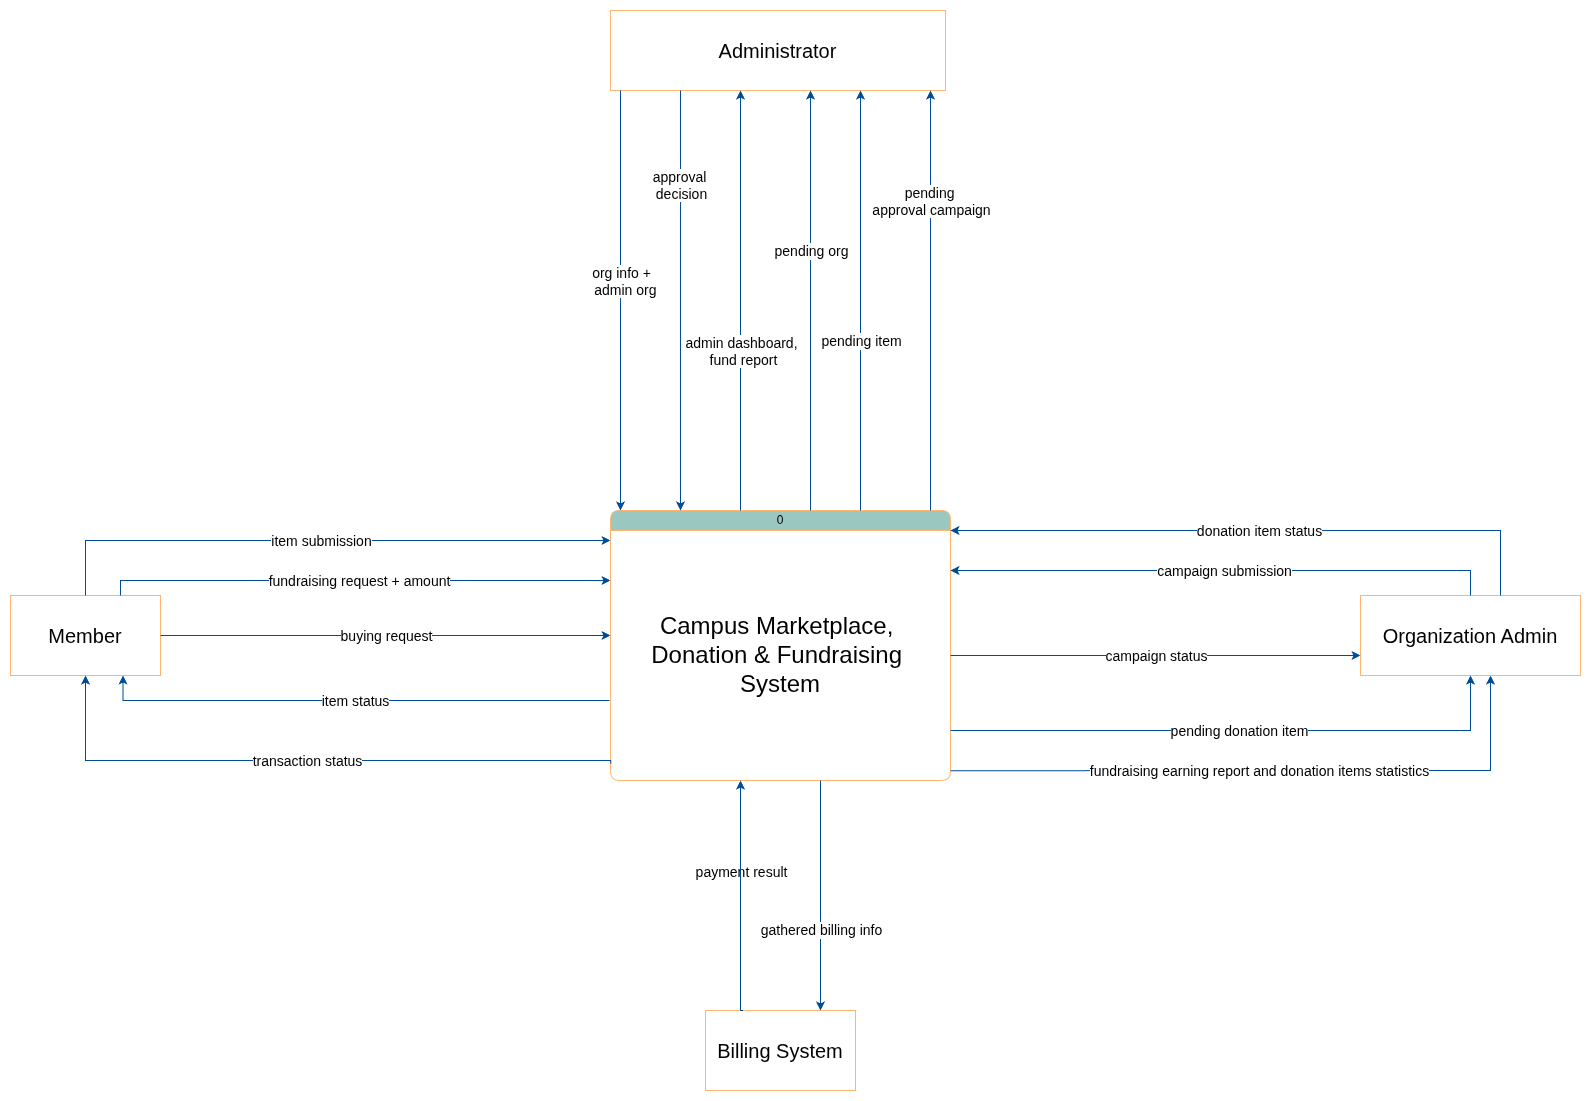
\includegraphics[width=0.75\textwidth]{context.drawio.png}
    \caption{Context Diagram}
    \label{fig:context-diagram}
\end{figure}

\section{Mô tả}
\subsection{Các Thực Thể Ngoài (External Entities)}

Hệ thống Campus Cycle tương tác với bốn thực thể bên ngoài chính, mỗi
thực thể đảm nhận một vai trò riêng trong quá trình vận hành và trao đổi dữ liệu
với hệ thống.

\textbf{Member}

Member là các thành viên sử dụng hệ thống, bao gồm học sinh và giáo viên
trong trường. Đây là nhóm người dùng chính tham gia vào các hoạt động như đăng
tải sản phẩm, gửi yêu cầu mua sản phẩm, tham gia các chiến dịch gây quỹ và theo
dõi trạng thái giao dịch. Phần lớn dữ liệu nghiệp vụ quan trọng như thông tin bài
đăng sản phẩm, yêu cầu mua hàng và yêu cầu quyên góp đều được khởi tạo từ
thực thể này.

\textbf{Administrator}

Administrator đóng vai trò quản trị viên hệ thống với quyền quản lý toàn bộ
hoạt động vận hành. Thực thể này chịu trách nhiệm quản lý tổ chức, phân quyền
quản trị viên tổ chức và thực hiện các quyết định kiểm duyệt hoặc từ chối đối
với các dữ liệu cần xét duyệt. Ngoài ra, Administrator còn tiếp nhận các báo cáo,
dashboard thống kê và danh sách dữ liệu đang chờ xử lý từ hệ thống.

\textbf{Organization Administrator}

Organization Administrator là quản trị viên đại diện cho các tổ chức, câu lạc
bộ hoặc đơn vị trong trường học. Thực thể này có quyền tạo và quản lý các chiến
dịch gây quỹ hoặc quyên góp, theo dõi trạng thái vật phẩm quyên góp và nhận các
báo cáo liên quan đến chiến dịch do tổ chức của mình phụ trách.

\textbf{Billing System}

Billing System là hệ thống thanh toán trung gian nằm ngoài hệ thống Campus
Cycle. Hệ thống này tiếp nhận thông tin thanh toán từ Campus Cycle để xử lý
giao dịch, sau đó trả về kết quả thanh toán và trạng thái giao dịch để hệ thống
cập nhật dữ liệu tương ứng.

\subsection{ Phân Tích Luồng Dữ Liệu (Context Data Flows)}

\subsubsection{Tương tác giữa Member và Campus Cycle}

Tương tác giữa Member và Campus Cycle Member là người dùng chính của
toàn bộ hệ thống Campus Cycle. Các luồng dữ liệu đi từ Member vào hệ thống
mang ý nghĩa đại diện cho hành động tạo dữ liệu hoặc gửi yêu cầu cần xử lý. Ngược
lại, các luồng từ hệ thống trả về giúp Member theo dõi kết quả của các quá trình
xử lý và xác định được bước tiếp theo cần làm.

\begin{table}[H]
\centering
\caption{Các luồng dữ liệu giữa Member và hệ thống}
\label{tab:member-system-data-flow}

\begin{tabular}{|p{4cm}|p{4cm}|p{7cm}|}
\hline
\textbf{Luồng dữ liệu} & \textbf{Hướng đi} & \textbf{Ý nghĩa} \\
\hline

item &
Member $\rightarrow$ System &
Member gửi thông tin chi tiết của sản phẩm cần đăng lên hệ thống, bao gồm dữ liệu mô tả sản phẩm, loại sản phẩm và các thông tin liên quan khác. \\
\hline

fundraising request + amount &
Member $\rightarrow$ System &
Member gửi yêu cầu muốn quyên góp tiền cho một chiến dịch gây quỹ, đi kèm với số tiền cụ thể muốn đóng góp. \\
\hline

buying request &
Member $\rightarrow$ System &
Member gửi yêu cầu xác nhận mua một sản phẩm hiện đang được đăng bán trên hệ thống. \\
\hline

item status &
System $\rightarrow$ Member &
Hệ thống phản hồi trạng thái hiện tại của sản phẩm như đang chờ duyệt, đã duyệt, bị từ chối hoặc hoàn tất. \\
\hline

transaction status &
System $\rightarrow$ Member &
Hệ thống phản hồi trạng thái giao dịch như đang chờ thanh toán, đã thanh toán hoặc hoàn tất. \\
\hline

\end{tabular}
\end{table}

\subsubsection{Tương tác giữa Administrator và Campus Cycle}

Tương tác giữa Administrator và Campus Cycle Administrator đóng vai trò
là người kiểm soát và quản trị toàn bộ hoạt động của hệ thống. Quy trình làm việc
chủ yếu của thực thể này là nhận các dữ liệu đang chờ xử lý từ hệ thống, sau đó
đưa ra và gửi lại quyết định duyệt/từ chối. Ngoài ra, Administrator còn nhận báo
cáo để theo dõi hoạt động chung của Campus Cycle.

\begin{table}[H]
\centering
\caption{Các luồng dữ liệu giữa Administrator và hệ thống}
\label{tab:admin-system-data-flow}

\begin{tabular}{|p{4cm}|p{4cm}|p{7cm}|}
\hline
\textbf{Luồng dữ liệu} & \textbf{Hướng đi} & \textbf{Ý nghĩa} \\
\hline

org info + admin org &
Administrator $\rightarrow$ System &
Administrator cung cấp cho hệ thống thông tin của các tổ chức, kèm theo thông tin của các thành viên được phân quyền làm quản trị viên cho tổ chức đó. \\
\hline

approval decision &
Administrator $\rightarrow$ System &
Administrator gửi lại hệ thống các quyết định kiểm duyệt, bao gồm duyệt hoặc từ chối các sản phẩm, chiến dịch hoặc dữ liệu đang chờ xử lý. \\
\hline

admin dashboard, fund report &
System $\rightarrow$ Administrator &
Hệ thống cung cấp bảng điều khiển tổng quan dashboard cùng các báo cáo liên quan đến quỹ và hoạt động của hệ thống. \\
\hline

pending org &
System $\rightarrow$ Administrator &
Hệ thống gửi danh sách các tổ chức hoặc thông tin tổ chức đang ở trạng thái chờ Administrator xử lý. \\
\hline

pending item &
System $\rightarrow$ Administrator &
Hệ thống gửi danh sách các sản phẩm đang chờ Administrator kiểm duyệt. \\
\hline

pending approval campaign &
System $\rightarrow$ Administrator &
Hệ thống gửi danh sách các chiến dịch đang chờ Administrator kiểm duyệt trước khi được công khai. \\
\hline

\end{tabular}
\end{table}

\subsubsection{Tương tác giữa Organization Admin và Campus Cycle}

Organization Admin là thực thể chịu trách nhiệm vận hành các chiến dịch ở cấp độ tổ chức. Họ thao tác để tạo chiến dịch, quản lý các vật phẩm quyên góp và theo dõi hiệu quả của các chiến dịch thông qua báo cáo do hệ thống cung cấp.

\begin{table}[H]
\centering
\caption{Các luồng dữ liệu giữa Organization Administrator và hệ thống}
\label{tab:org-admin-system-data-flow}

\begin{tabular}{|p{4cm}|p{4cm}|p{7cm}|}
\hline
\textbf{Luồng dữ liệu} & \textbf{Hướng đi} & \textbf{Ý nghĩa} \\
\hline

campaign &
Organization Admin $\rightarrow$ System &
Organization Admin gửi thông tin của một chiến dịch mới, bao gồm tên, mô tả, thời gian, loại chiến dịch và các dữ liệu liên quan. \\
\hline

donation item status &
Organization Admin $\rightarrow$ System &
Organization Admin cập nhật vào hệ thống trạng thái của các vật phẩm quyên góp, ví dụ như chấp nhận, chờ bàn giao, đã nhận hoặc từ chối. \\
\hline

campaign status &
System $\rightarrow$ Organization Admin &
Hệ thống trả lại trạng thái của chiến dịch sau khi xử lý hoặc sau khi được Administrator kiểm duyệt. \\
\hline

pending donation item &
System $\rightarrow$ Organization Admin &
Hệ thống gửi danh sách các vật phẩm quyên góp đang chờ Organization Admin xem xét hoặc xử lý. \\
\hline

fundraising earning report and donation items statistics &
System $\rightarrow$ Organization Admin &
Hệ thống cung cấp báo cáo về số tiền gây quỹ và thống kê chi tiết về các vật phẩm quyên góp cho Organization Admin. \\
\hline

\end{tabular}
\end{table}

\subsubsection{Tương tác giữa Billing System và Campus Cycle}

Campus Cycle không trực tiếp thực hiện việc xử lý thông tin thanh toán chi tiết. Thay vào đó, Billing System là hệ thống ngoài được dùng để đảm nhận nhiệm vụ này. Campus Cycle chỉ gửi dữ liệu cần thiết sang và nhận lại kết quả xử lý từ Billing System.

\begin{table}[H]
\centering
\caption{Các luồng dữ liệu giữa Billing System và hệ thống}
\label{tab:billing-system-data-flow}

\begin{tabular}{|p{4cm}|p{4cm}|p{7cm}|}
\hline
\textbf{Luồng dữ liệu} & \textbf{Hướng đi} & \textbf{Ý nghĩa} \\
\hline

gathered billing info &
System $\rightarrow$ Billing System &
Hệ thống tổng hợp thông tin hóa đơn hoặc dữ liệu thanh toán và gửi sang Billing System để thực hiện xử lý thanh toán. \\
\hline

payment result &
Billing System $\rightarrow$ System &
Billing System trả về thông tin chi tiết thanh toán cùng trạng thái giao dịch để Campus Cycle cập nhật kết quả giao dịch trong hệ thống. \\
\hline

\end{tabular}
\end{table}

\chapter{Sơ đồ Luồng dữ liệu}

\section{Data Flow Diagram Level 0}

\subsection{ DFD Level 0}

\begin{figure}[H]
    \centering
    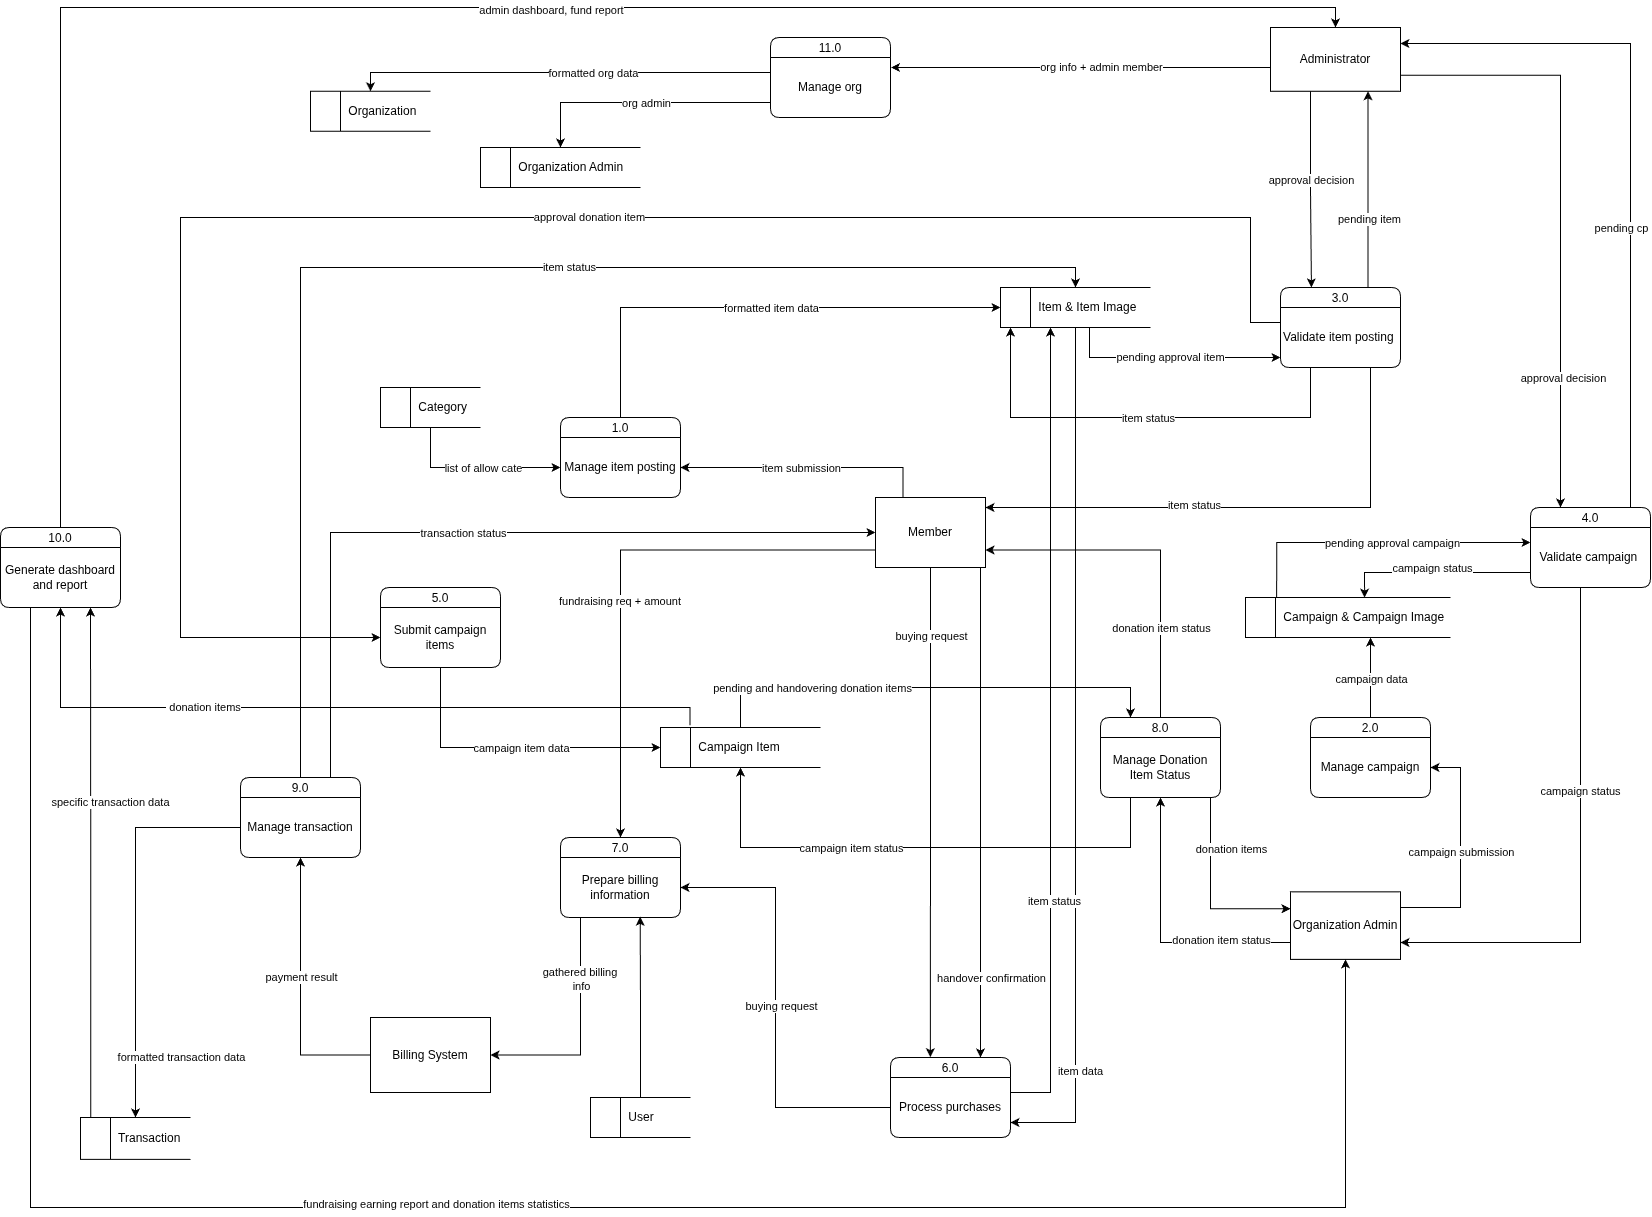
\includegraphics[width=0.75\textwidth]{dfd0.drawio.png}
    \caption{DFD Level 0}
    \label{fig:dfd-level-0}
\end{figure}

\subsection{ Chi tiết các tiến trình trên DFD Level-0}

\textbf{P1.0 -- Manage Item Posting}

\textit{Tác dụng:} Tiếp nhận bài đăng sản phẩm từ Member, kiểm tra danh mục được phép từ Category và chuẩn hóa dữ liệu trước khi lưu vào \textbf{Item} và \textbf{Item Image} để chờ kiểm duyệt.

\textbf{P2.0 -- Manage Campaign}

\textit{Tác dụng:} Tiếp nhận thông tin chiến dịch từ Organization Administrator, chuẩn hóa dữ liệu và lưu vào \textbf{Campaign} và \textbf{Campaign Image} ở trạng thái chờ duyệt.

\textbf{P3.0 -- Validate Item Posting}

\textit{Tác dụng:} Xử lý kiểm duyệt bài đăng sản phẩm dựa trên dữ liệu \textbf{pending item} và quyết định của Administrator; cập nhật trạng thái sản phẩm và thông báo kết quả cho Member.

\textbf{P4.0 -- Validate Campaign}

\textit{Tác dụng:} Xử lý kiểm duyệt chiến dịch dựa trên dữ liệu \textbf{pending campaign} và quyết định của Administrator; cập nhật trạng thái chiến dịch và thông báo kết quả cho Organization Administrator.

\textbf{P5.0 -- Submit Campaign Items}

\textit{Tác dụng:} Liên kết vật phẩm quyên góp đã được kiểm duyệt với chiến dịch phù hợp, tạo và cập nhật dữ liệu \textbf{Campaign Item} để Organization Administrator tiếp tục xử lý bàn giao.

\textbf{P6.0 -- Process Purchases}

\textit{Tác dụng:} Xử lý yêu cầu mua sản phẩm từ Member, kiểm tra trạng thái sản phẩm và cập nhật trạng thái khi có thay đổi trong quá trình mua hoặc bàn giao.

\textbf{P7.0 -- Prepare Billing Information}

\textit{Tác dụng:} Tổng hợp dữ liệu người dùng, số tiền và ngữ cảnh giao dịch để tạo thông tin hóa đơn gửi sang Billing System.

\textbf{P8.0 -- Manage Donation Item Status}

\textit{Tác dụng:} Quản lý quá trình kiểm duyệt và bàn giao vật phẩm quyên góp, cập nhật trạng thái \textbf{Campaign Item} và thông báo kết quả cho Member.

\textbf{P9.0 -- Manage Transaction}

\textit{Tác dụng:} Ghi nhận kết quả thanh toán từ Billing System, lưu dữ liệu giao dịch vào \textbf{Transaction}, cập nhật trạng thái sản phẩm và thông báo trạng thái giao dịch cho Member.

\textbf{P10.0 -- Generate Dashboard and Report}

\textit{Tác dụng:} Tạo dashboard, báo cáo quỹ, báo cáo doanh thu gây quỹ và thống kê vật phẩm quyên góp dựa trên dữ liệu \textbf{Transaction} và \textbf{Campaign Item}.

\textbf{P11.0 -- Manage Organization}

\textit{Tác dụng:} Quản lý dữ liệu tổ chức và phân công thành viên làm Organization Administrator theo thông tin do Administrator cung cấp.

\section{Data Flow Diagram Level 1}

\subsection{Process 1.0- Manage item posting}

\begin{figure}[H]
    \centering
    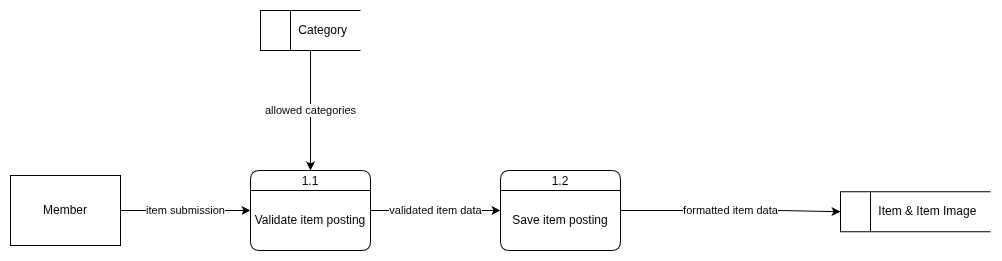
\includegraphics[width=0.75\textwidth]{dfd1-1.drawio.png}
    \caption{Process 1.0- Manage item posting}
    \label{fig:dfd-level-1-1}
\end{figure}

\subsection{Process 3.0- Validate item posting}

\begin{figure}[H]
    \centering
    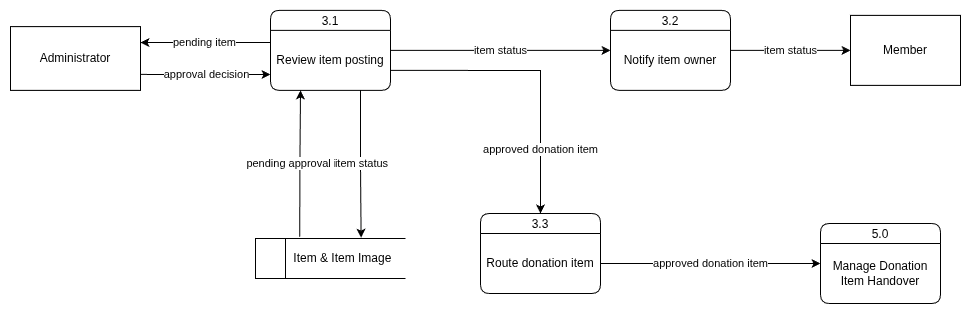
\includegraphics[width=0.75\textwidth]{dfd1-3.drawio.png}
    \caption{Process 3.0- Validate item posting}
    \label{fig:dfd-level-1-3}
\end{figure}

\subsection{Process 4.0- Validate campaign}

\begin{figure}[H]
    \centering
    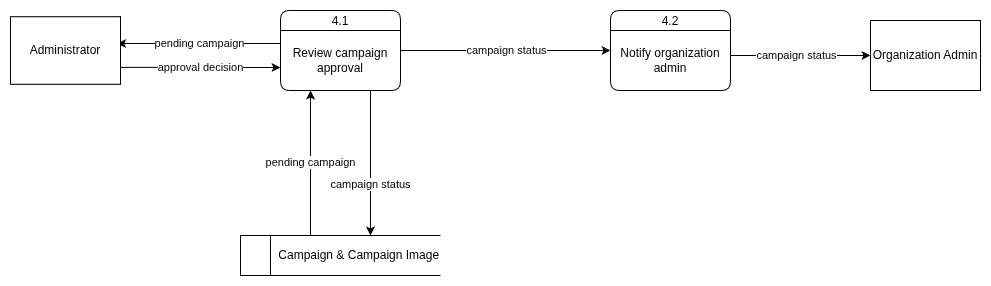
\includegraphics[width=0.75\textwidth]{dfd1-4.drawio.png}
    \caption{Process 4.0- Validate campaign}
    \label{fig:dfd-level-1-4}
\end{figure}

\subsection{Process 6.0- Process purchases}

\begin{figure}[H]
    \centering
    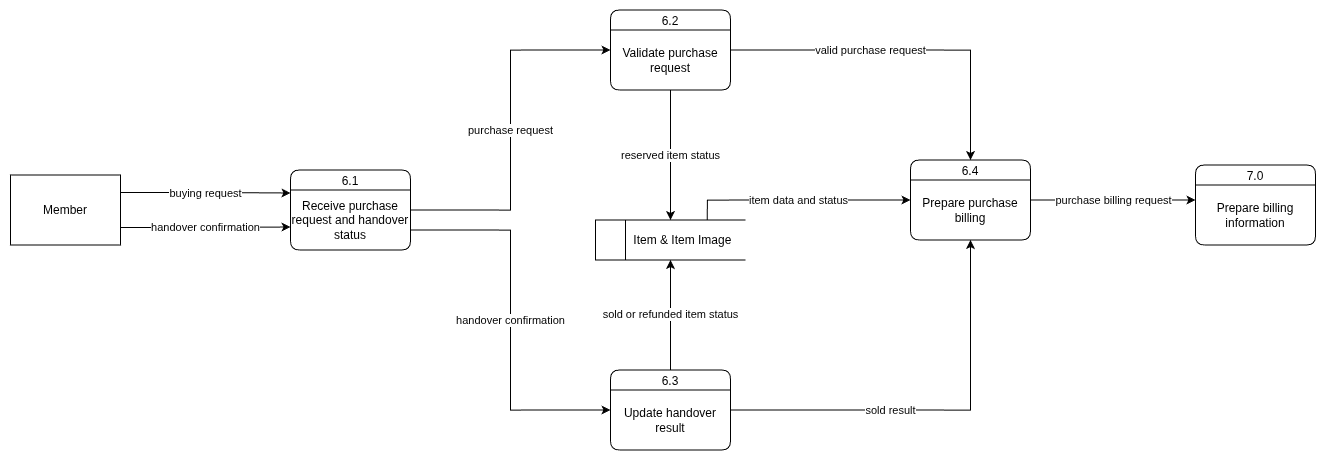
\includegraphics[width=0.75\textwidth]{dfd1-6.drawio.png}
    \caption{Process 6.0- Process purchases}
    \label{fig:dfd-level-1-6}
\end{figure}

\subsection{Process 8.0- Manage Donation Item Status}

\begin{figure}[H]
    \centering
    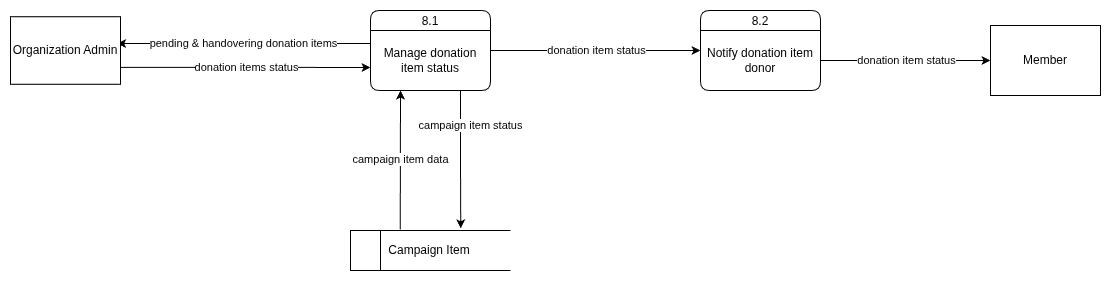
\includegraphics[width=0.75\textwidth]{dfd1-8.drawio.png}
    \caption{Process 8.0- Manage Donation Item Status}
    \label{fig:dfd-level-1-8}
\end{figure}

\subsection{Process 9.0- Manage transaction}

\begin{figure}[H]
    \centering
    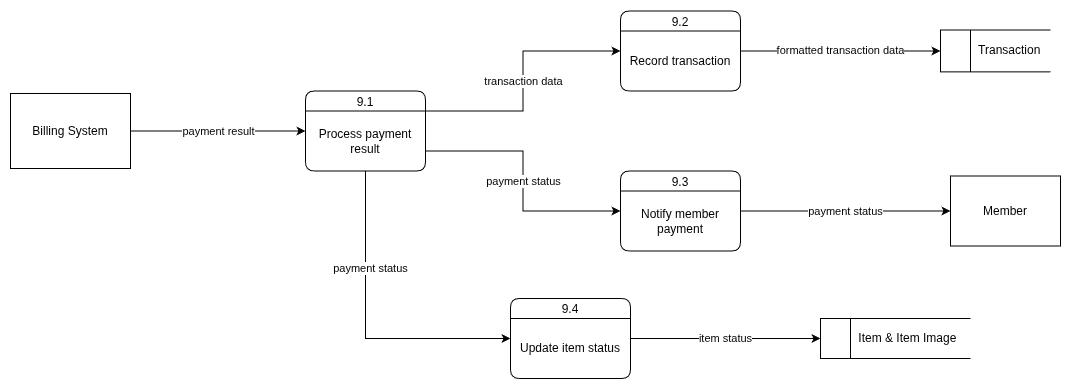
\includegraphics[width=0.75\textwidth]{dfd1-9.drawio.png}
    \caption{Process 9.0- Manage transaction}
    \label{fig:dfd-level-1-9}
\end{figure}

\chapter{Thiết kế Cơ sở dữ liệu}

\section{Thiết kế Cơ sở dữ liệu mức khái niệm (E-R Diagram)}

\begin{figure}[H]
    \centering
    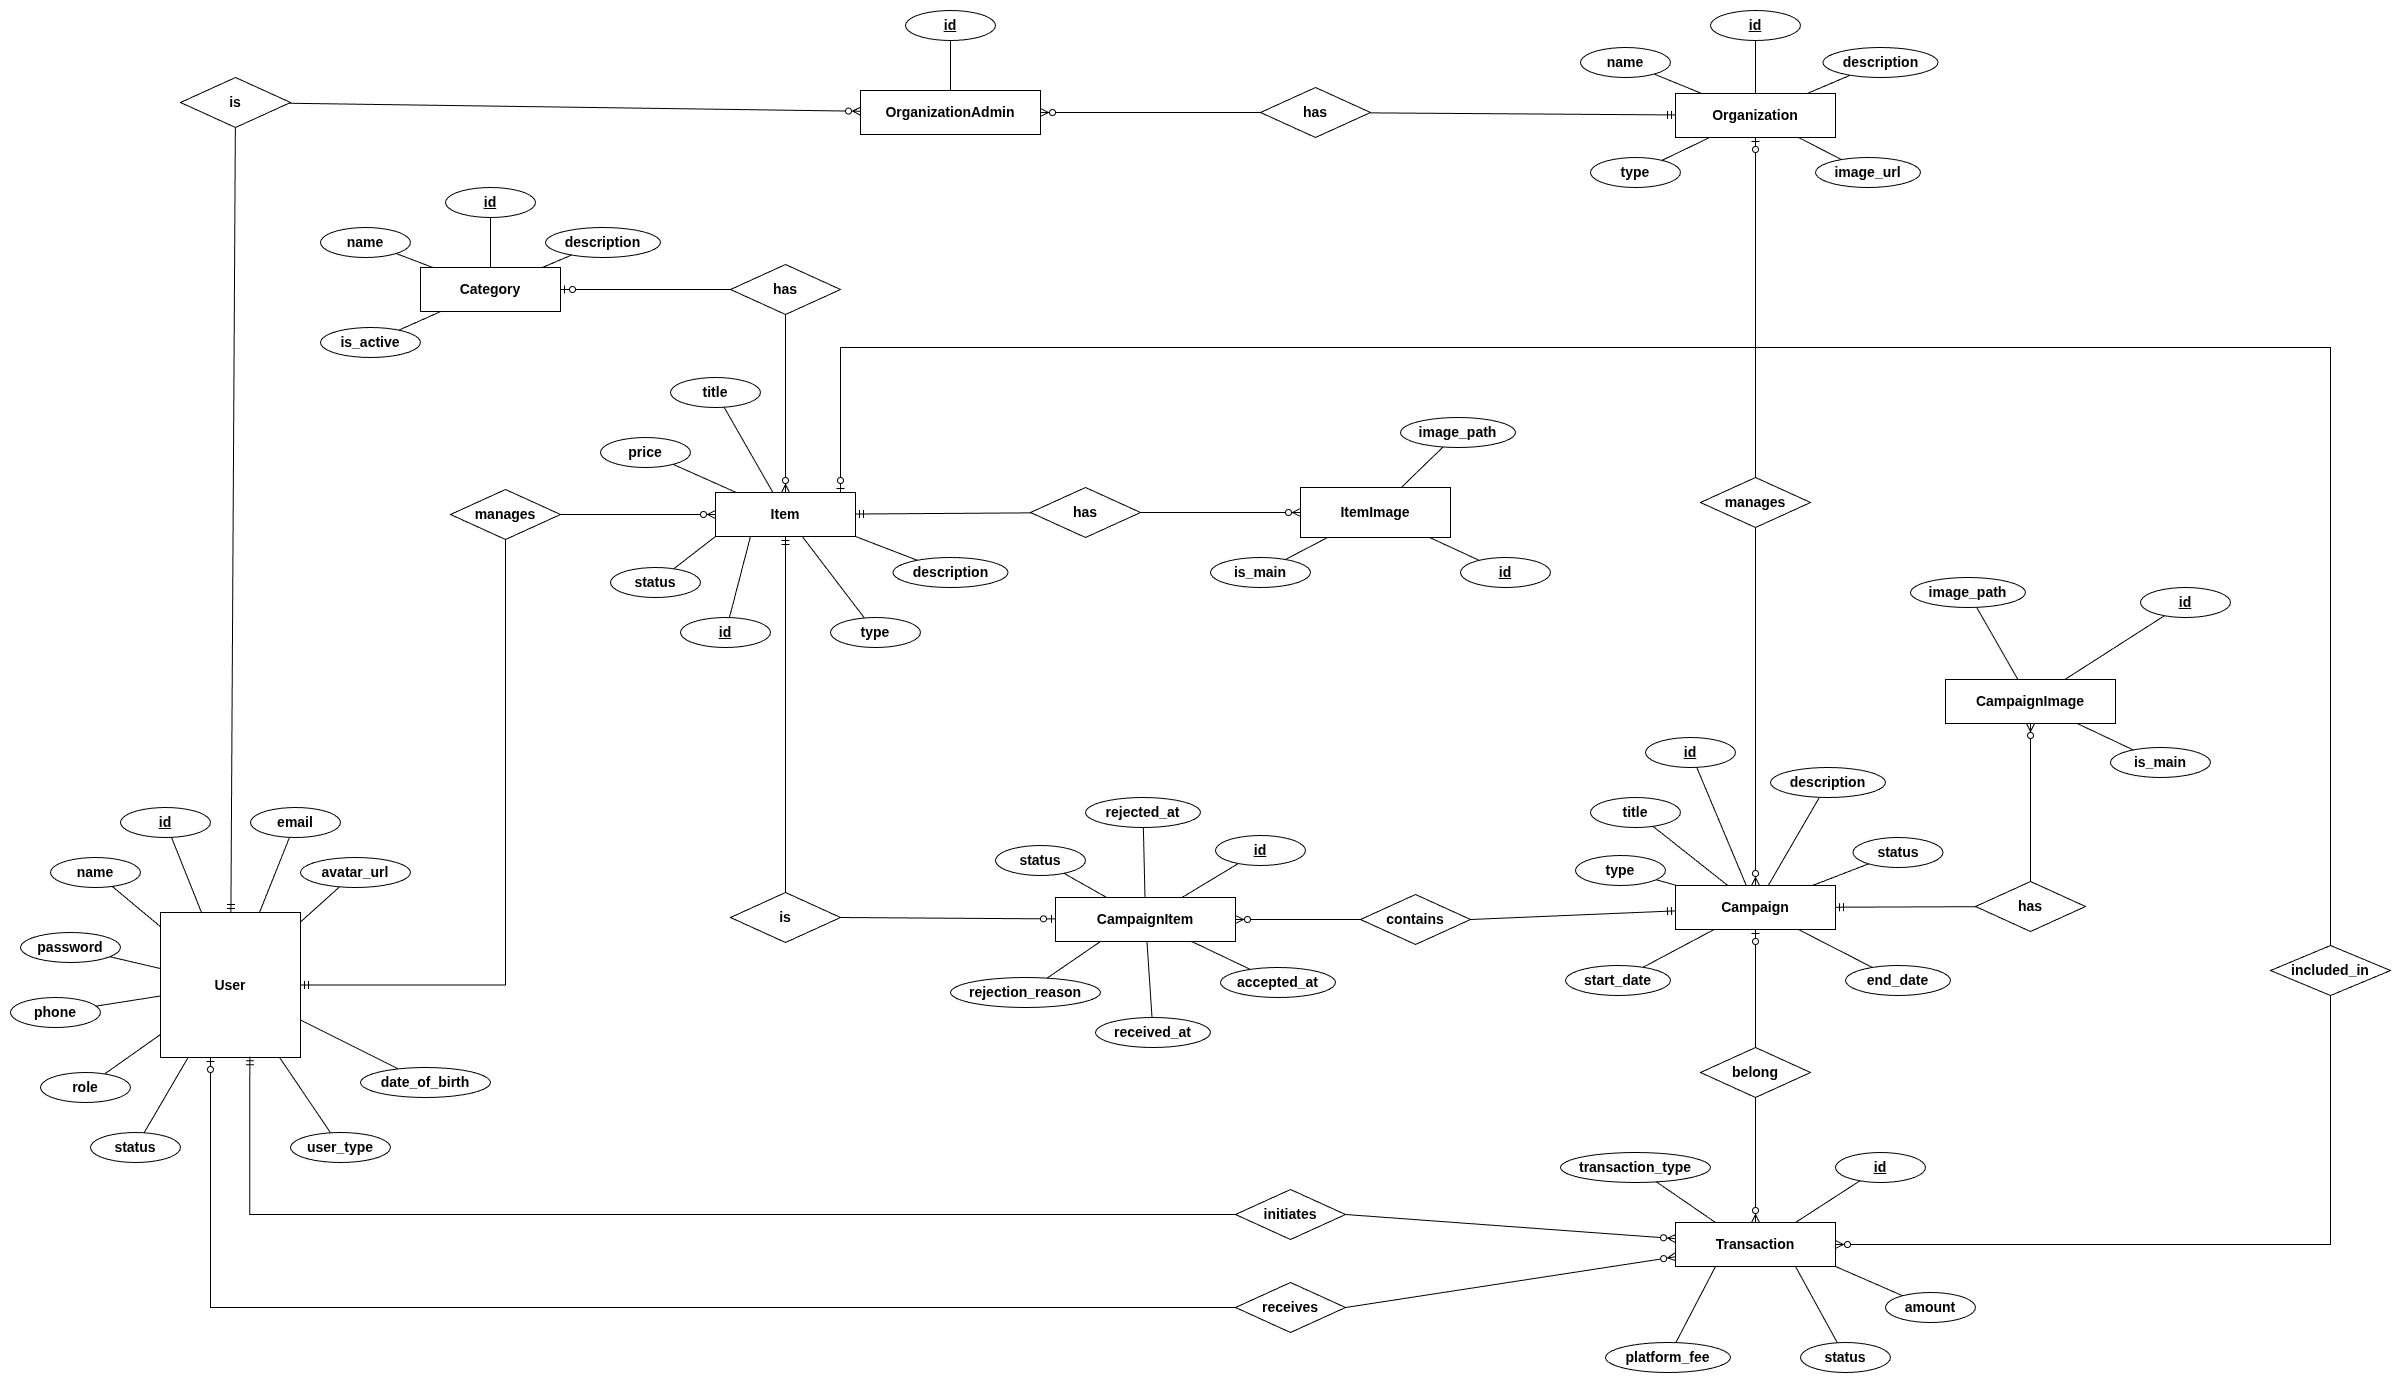
\includegraphics[width=0.75\textwidth]{er.drawio.png}
    \caption{E-R Diagram}
    \label{fig:er-diagram}
\end{figure}

\section{Thiết kế Cơ sở dữ liệu mức logic (Relational Diagram)}

\begin{figure}[H]
    \centering
    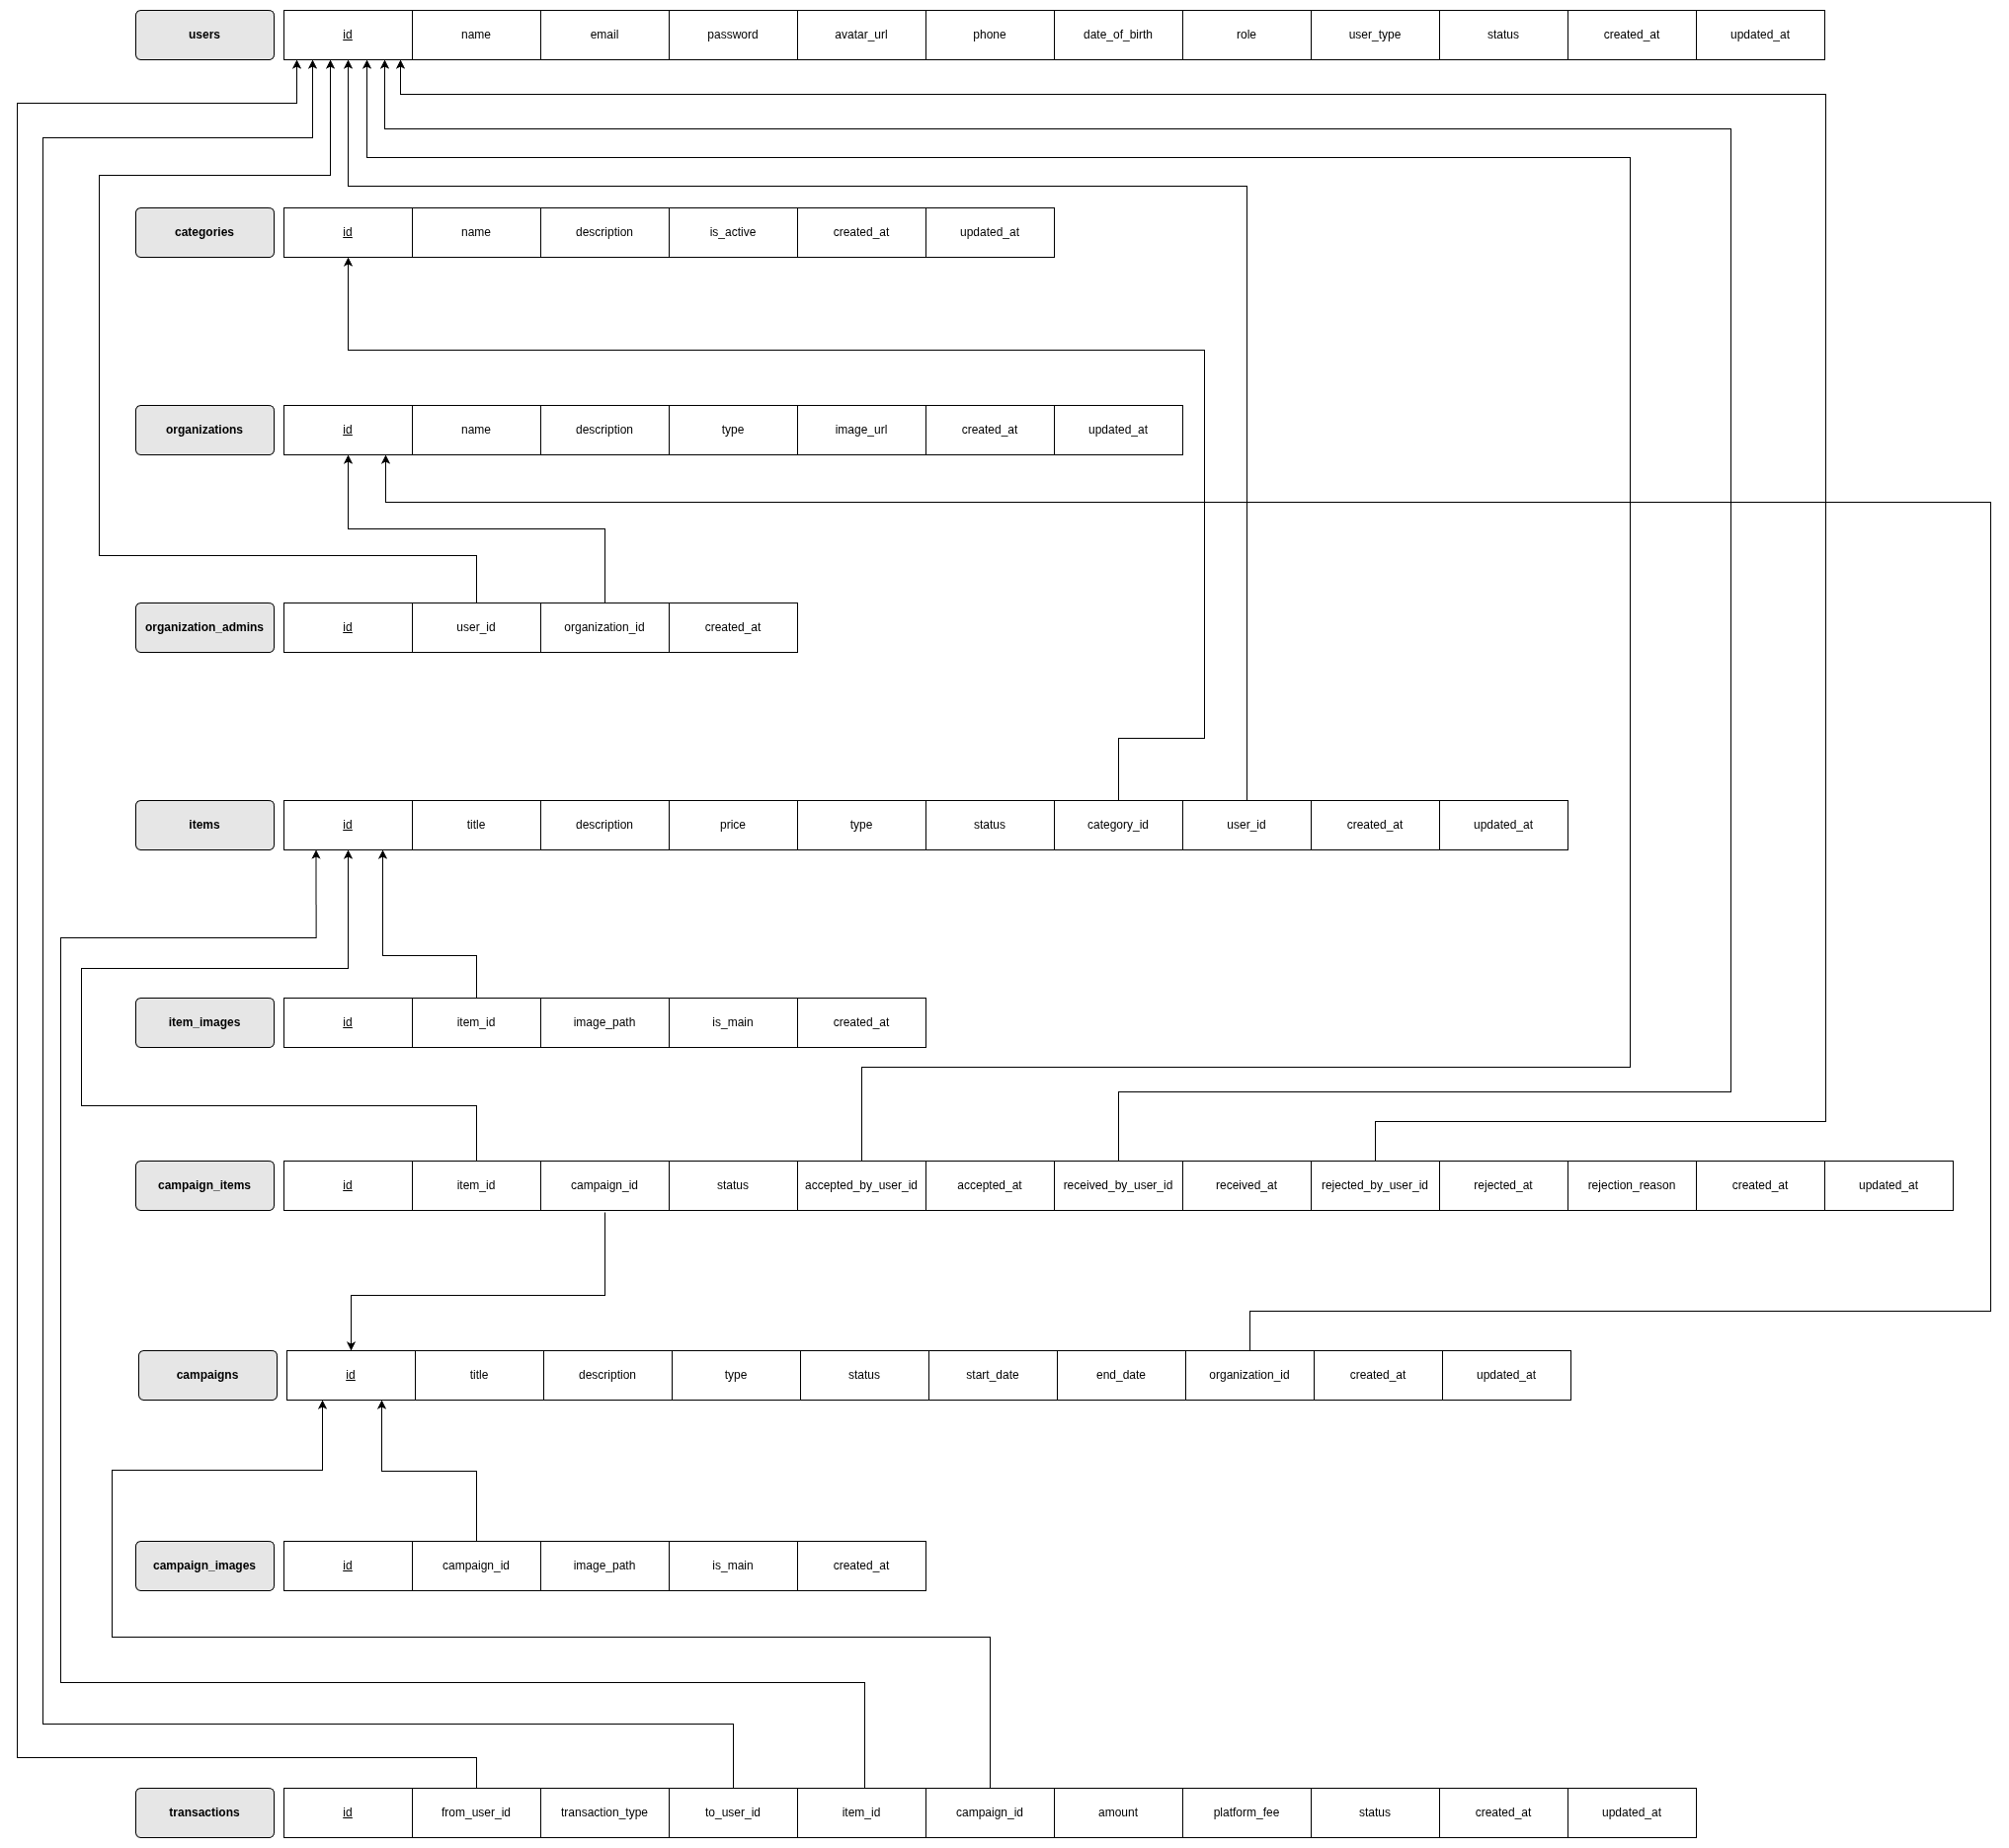
\includegraphics[width=0.75\textwidth]{rd.drawio.png}
    \caption{Relational Diagram}
    \label{fig:relational-diagram}
\end{figure}

\chapter{Triển khai và thực hiện}

\section{Cài đặt cơ sở dữ liệu}

\subsection{Cơ sở dữ liệu hệ thống}

Hệ thống sử dụng PostgreSQL 16 làm hệ quản trị cơ sở dữ liệu chính. PostgreSQL được lựa chọn nhờ khả năng quản lý dữ liệu quan hệ hiệu quả, hỗ trợ đầy đủ các ràng buộc toàn vẹn dữ liệu như khóa chính (Primary Key), khóa ngoại (Foreign Key), cùng nhiều kiểu dữ liệu hiện đại như UUID, Timestamp và Decimal. Ngoài ra, PostgreSQL có khả năng mở rộng tốt, độ ổn định cao và phù hợp với các hệ thống web có nhiều bảng dữ liệu liên kết với nhau.

Các bảng dữ liệu chính của hệ thống bao gồm:

\begin{itemize}[label=--, leftmargin=1.2cm]

\item \textbf{users}: Lưu thông tin tài khoản người dùng, vai trò, trạng thái tài khoản và các thông tin hồ sơ cá nhân.

\item \textbf{organizations}: Lưu thông tin về các tổ chức, câu lạc bộ hoặc đơn vị tham gia sử dụng hệ thống.

\item \textbf{organization\_admins}: Lưu mối quan hệ giữa người dùng và tổ chức mà họ được phân quyền quản trị.

\item \textbf{categories}: Lưu danh mục các loại vật phẩm được phép đăng tải trên hệ thống.

\item \textbf{items}: Lưu thông tin chi tiết về các vật phẩm được đăng bán hoặc quyên góp.

\item \textbf{item\_images}: Lưu đường dẫn và thông tin các hình ảnh liên quan đến vật phẩm.

\item \textbf{campaigns}: Lưu thông tin về các chiến dịch gây quỹ hoặc quyên góp được tạo trong hệ thống.

\item \textbf{campaign\_images}: Lưu hình ảnh minh họa cho các chiến dịch.

\item \textbf{campaign\_items}: Lưu thông tin các vật phẩm được đóng góp vào từng chiến dịch.

\item \textbf{transactions}: Lưu thông tin các giao dịch mua bán, quyên góp tiền và kết quả thanh toán.


\end{itemize}

Các bảng dữ liệu trên được liên kết với nhau thông qua các khóa ngoại nhằm đảm bảo tính nhất quán dữ liệu, hỗ trợ hiệu quả cho các chức năng quản lý người dùng, quản lý vật phẩm, quản lý chiến dịch, xử lý giao dịch và thống kê báo cáo của hệ thống.

\section{Giao diện cơ bản}
\subsection{Nhóm giao diện xác thực tài khoản}

Nhóm giao diện này phục vụ quá trình người dùng truy cập vào hệ thống. Người dùng có thể đăng nhập bằng tài khoản đã có hoặc tạo tài khoản mới để sử dụng các chức năng của hệ thống.

Login: Người dùng nhập email và mật khẩu để đăng nhập vào hệ thống.

\begin{figure}[H]
\centering
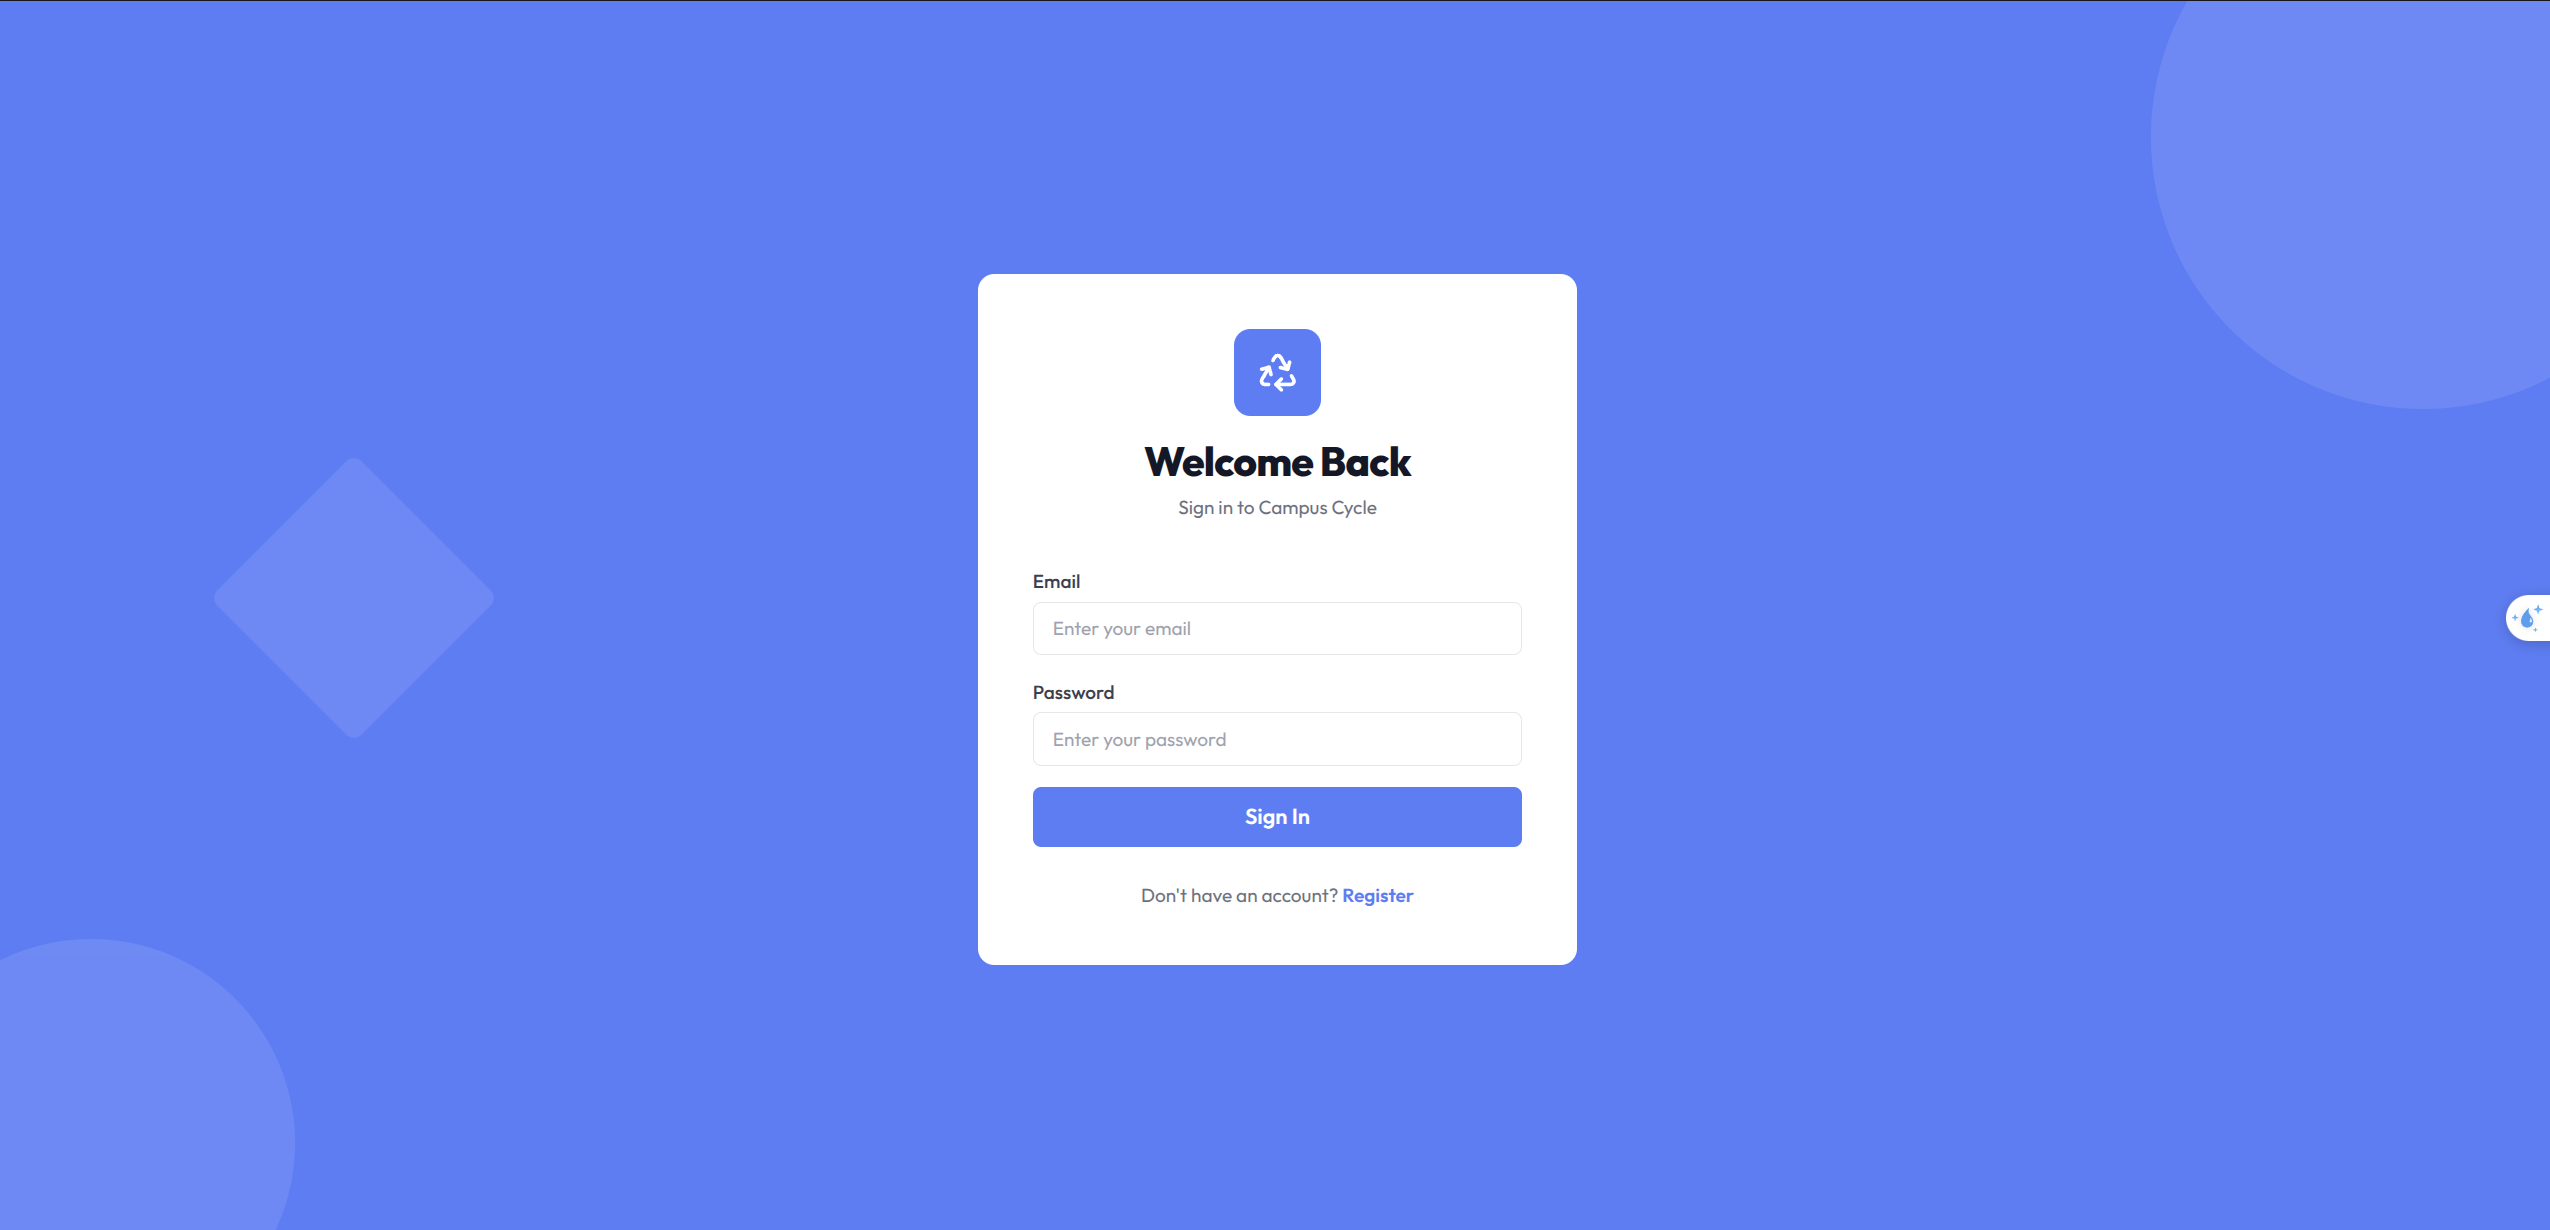
\includegraphics[width=0.75\textwidth]{Login Page.png}
\caption{Login Page}
\label{fig:login-page}
\end{figure}

Register: Người dùng tạo tài khoản mới bằng cách nhập thông tin cá nhân cần thiết.

\begin{figure}[H]
\centering
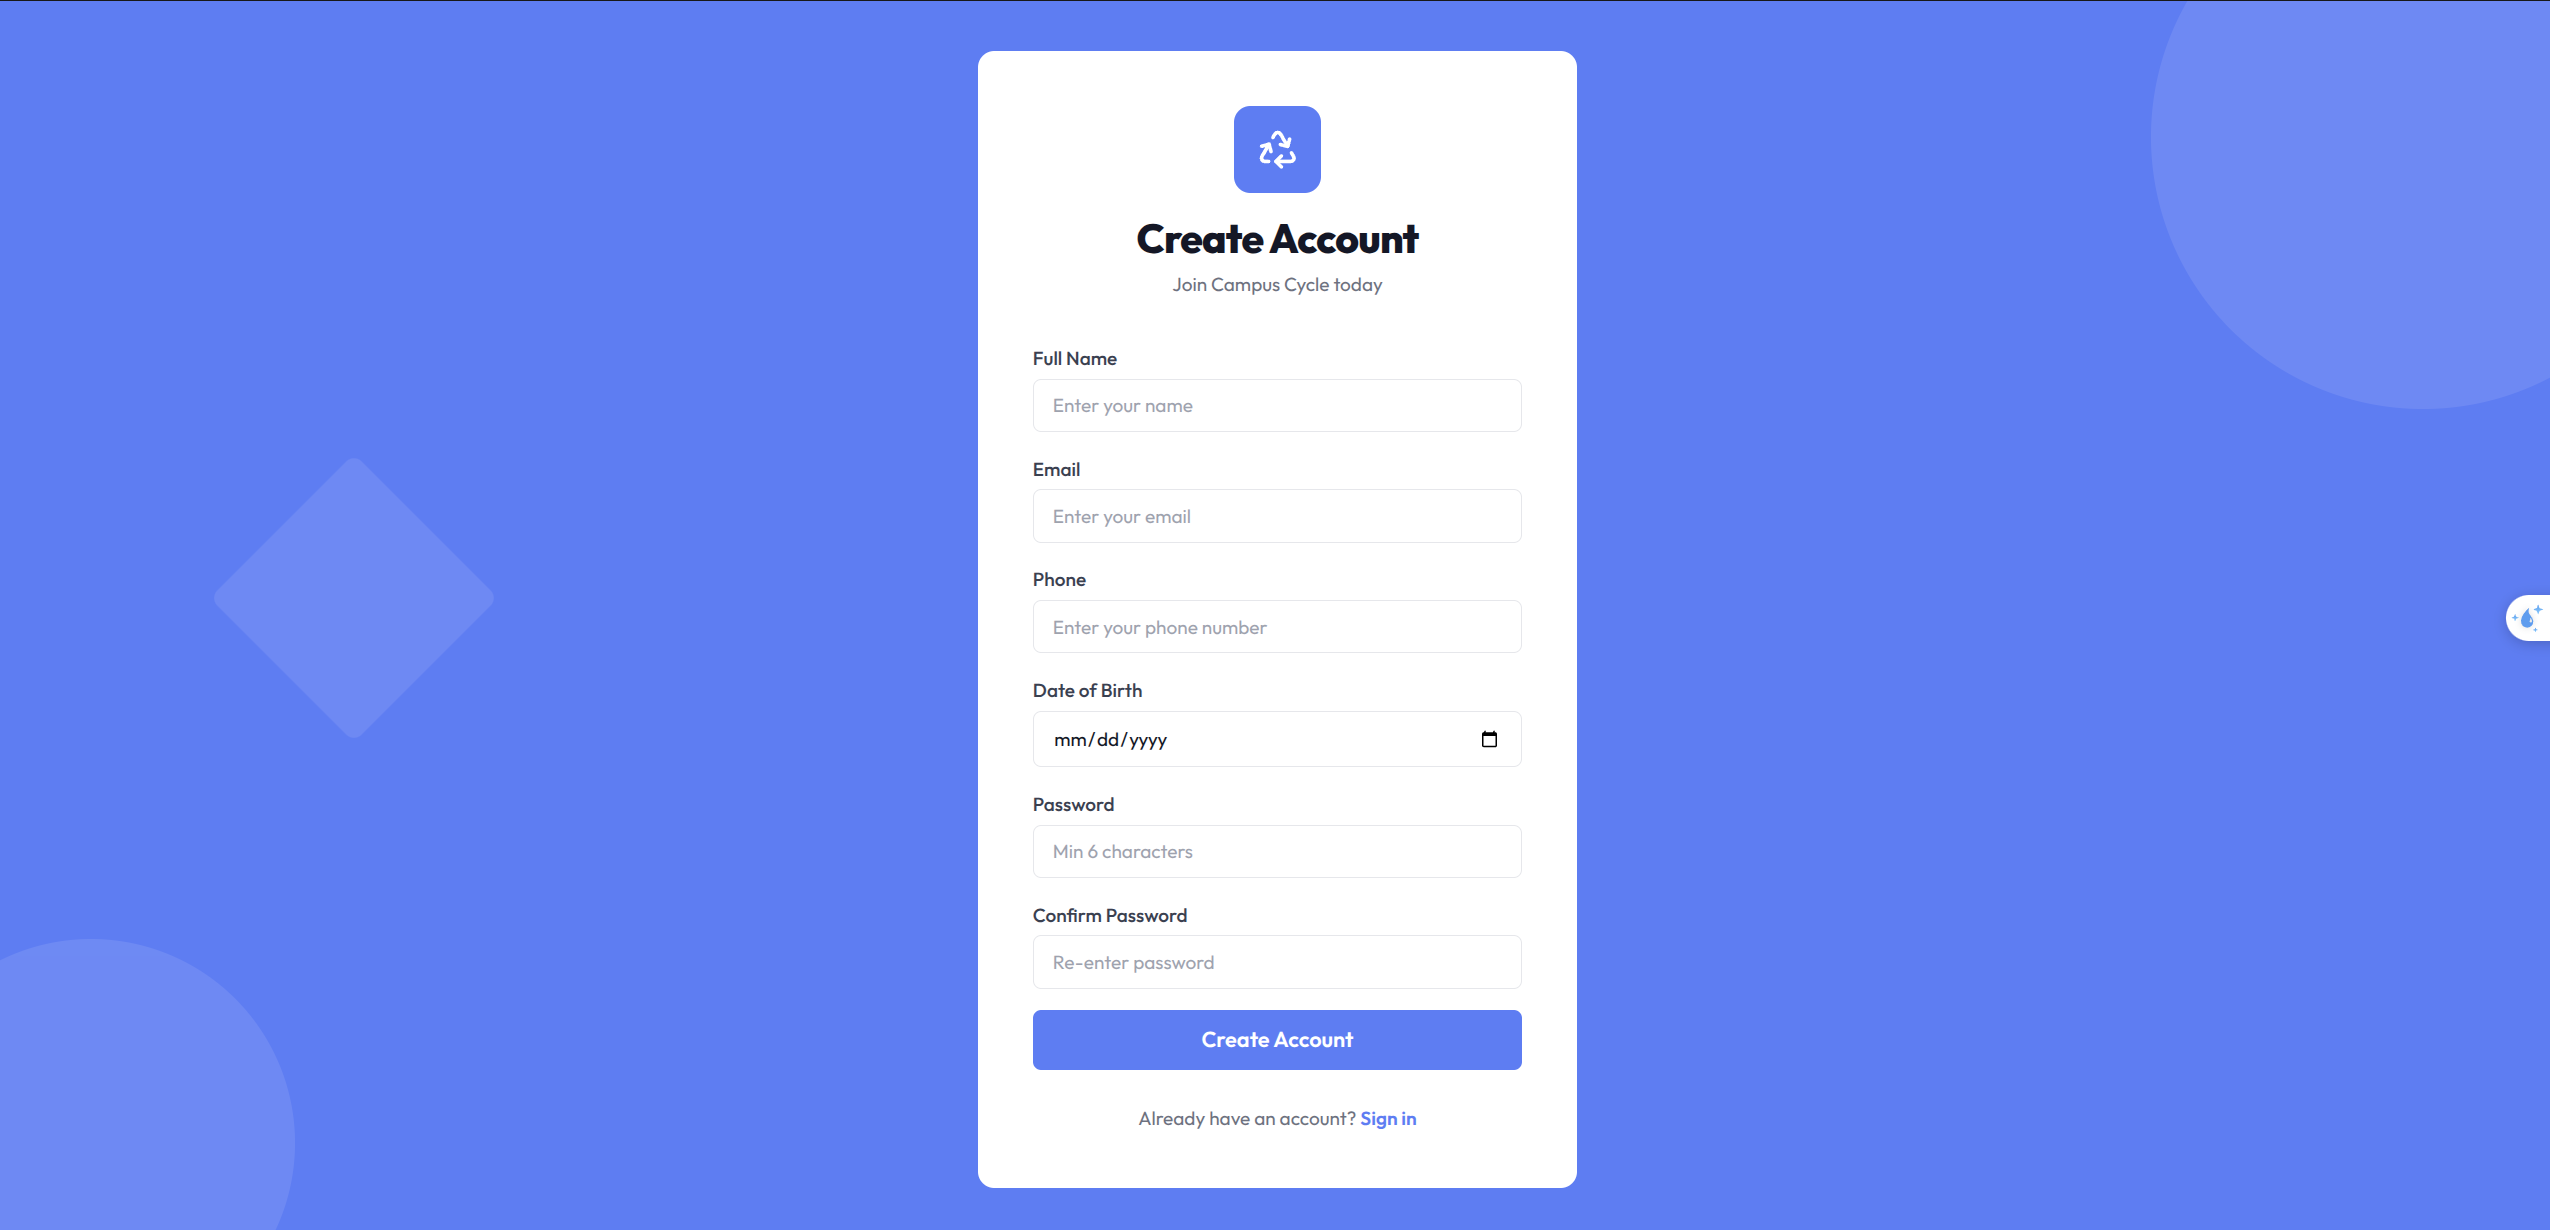
\includegraphics[width=0.75\textwidth]{Register Page.png}
\caption{Register Page}
\label{fig:register-page}
\end{figure}

\subsection{Nhóm giao diện thành viên}

Nhóm giao diện này dành cho Member, là người dùng thông thường của hệ thống. Member có thể xem trang chủ, xem danh sách vật phẩm, xem chi tiết vật phẩm, thực hiện quy trình mua hàng, đăng bán vật phẩm, quyên góp vật phẩm, quyên góp tiền cho campaign, quản lý hồ sơ cá nhân và theo dõi các vật phẩm hoặc đơn mua của mình.

Home Page: Hiển thị overview của hệ thống, các item và campaign nổi bật.

\begin{figure}[H]
\centering
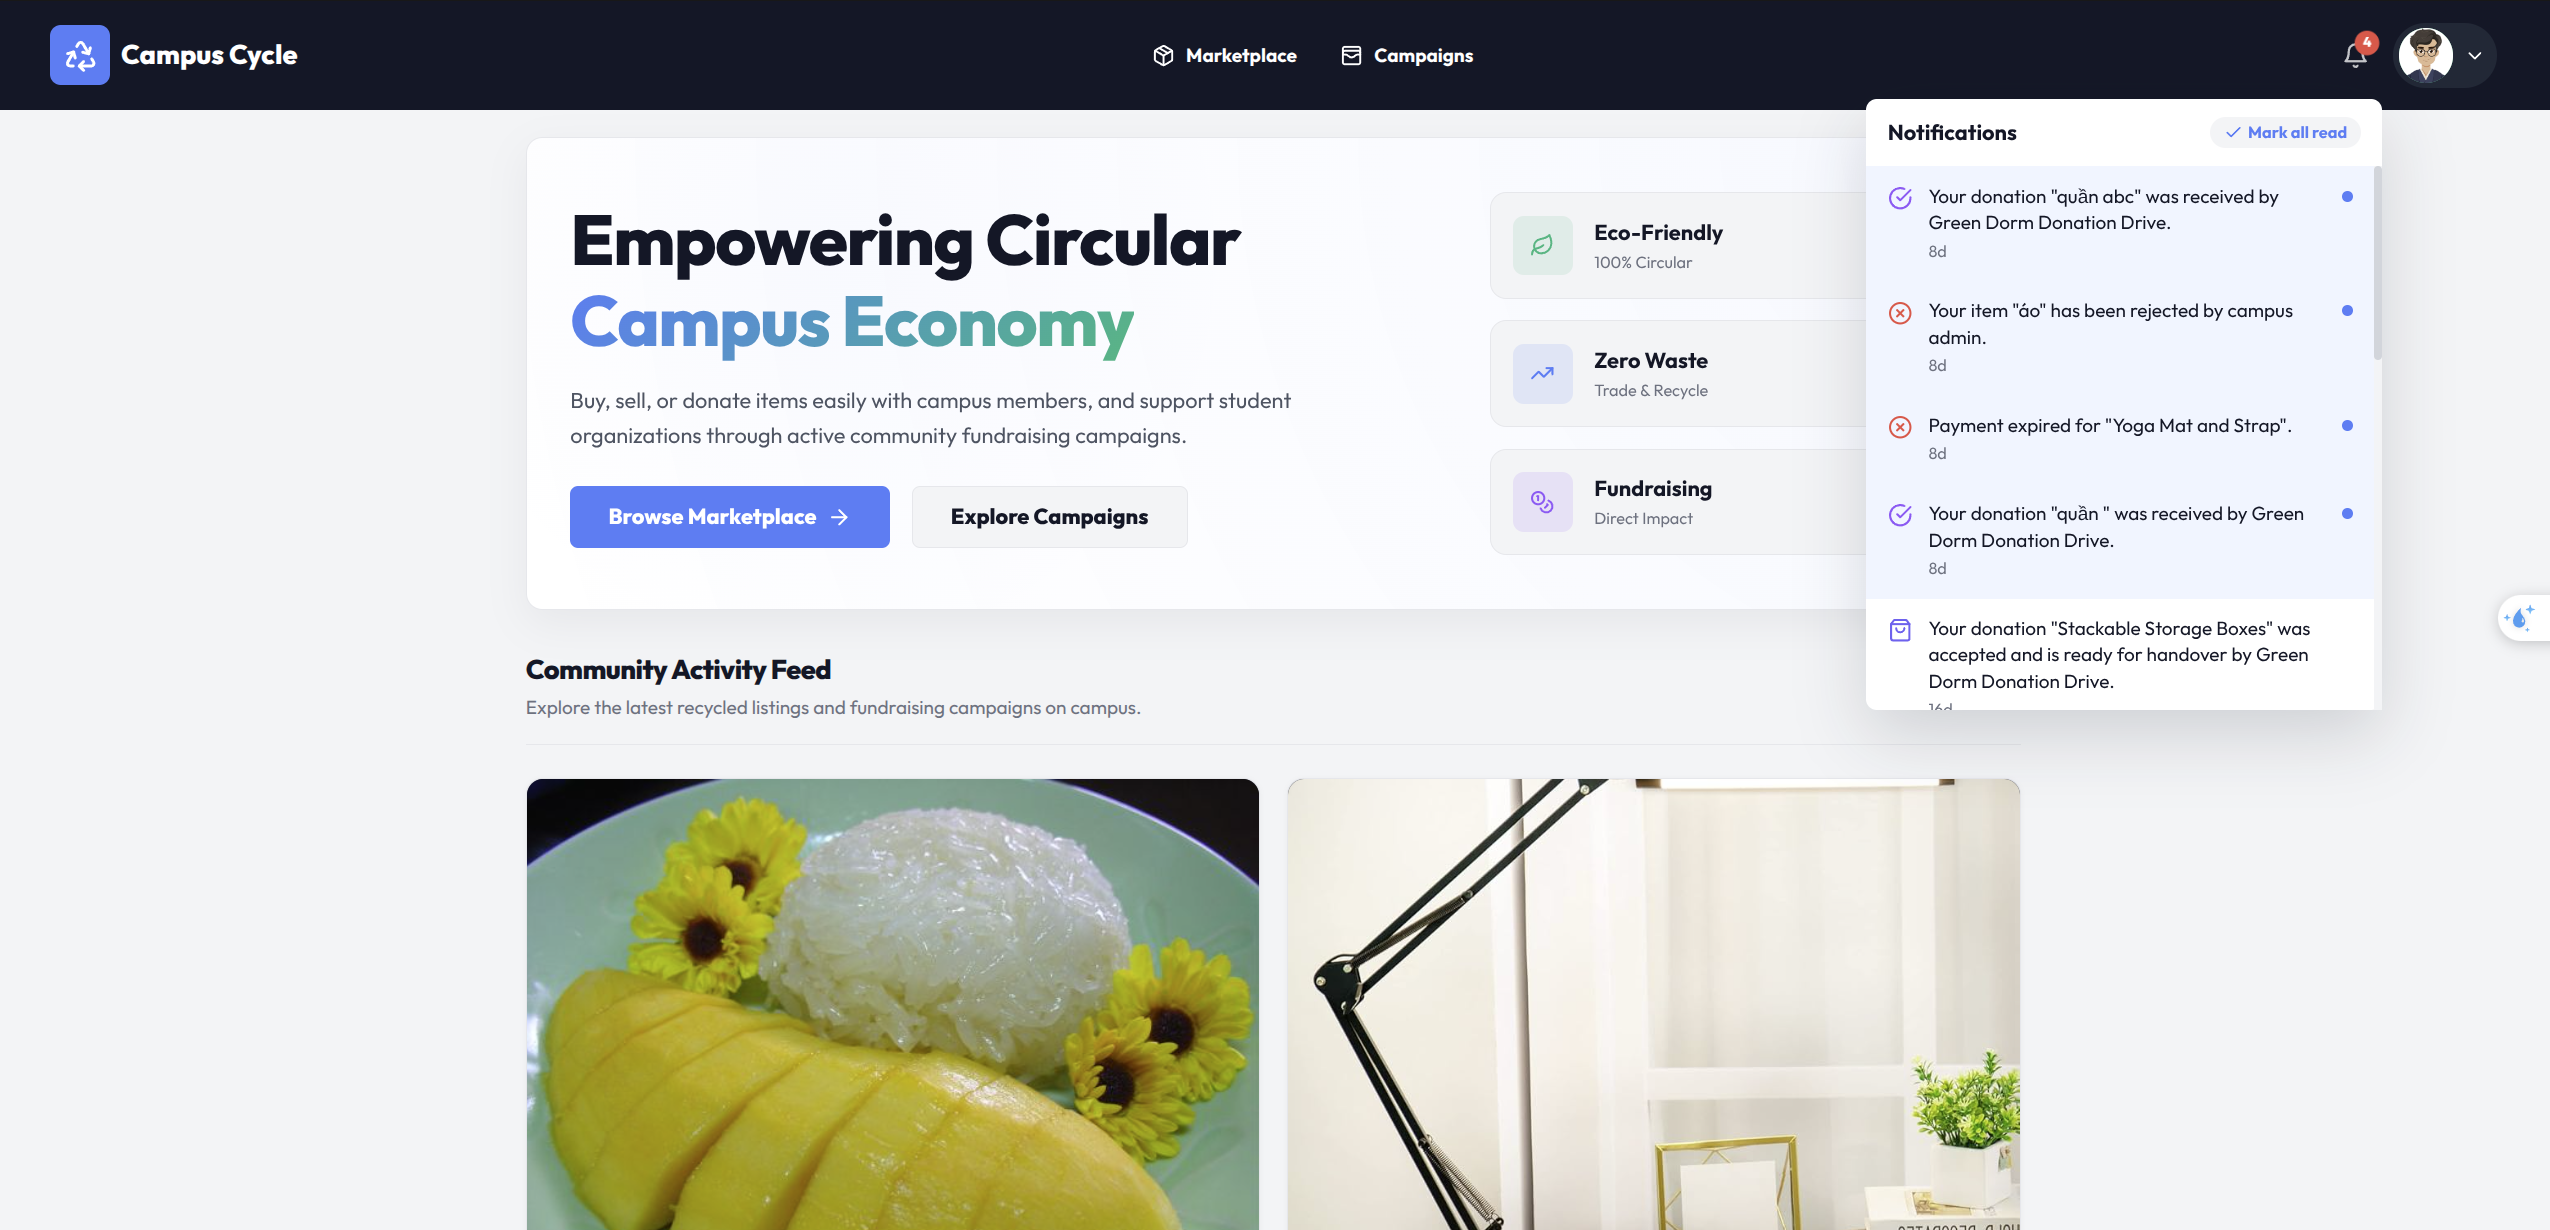
\includegraphics[width=0.75\textwidth]{Home Page.png}
\caption{Home Page}
\label{fig:home-page}
\end{figure}


Item Detail Page: Hiển thị thông tin chi tiết của item như hình ảnh, tên, giá và mô tả.

\begin{figure}[H]
\centering
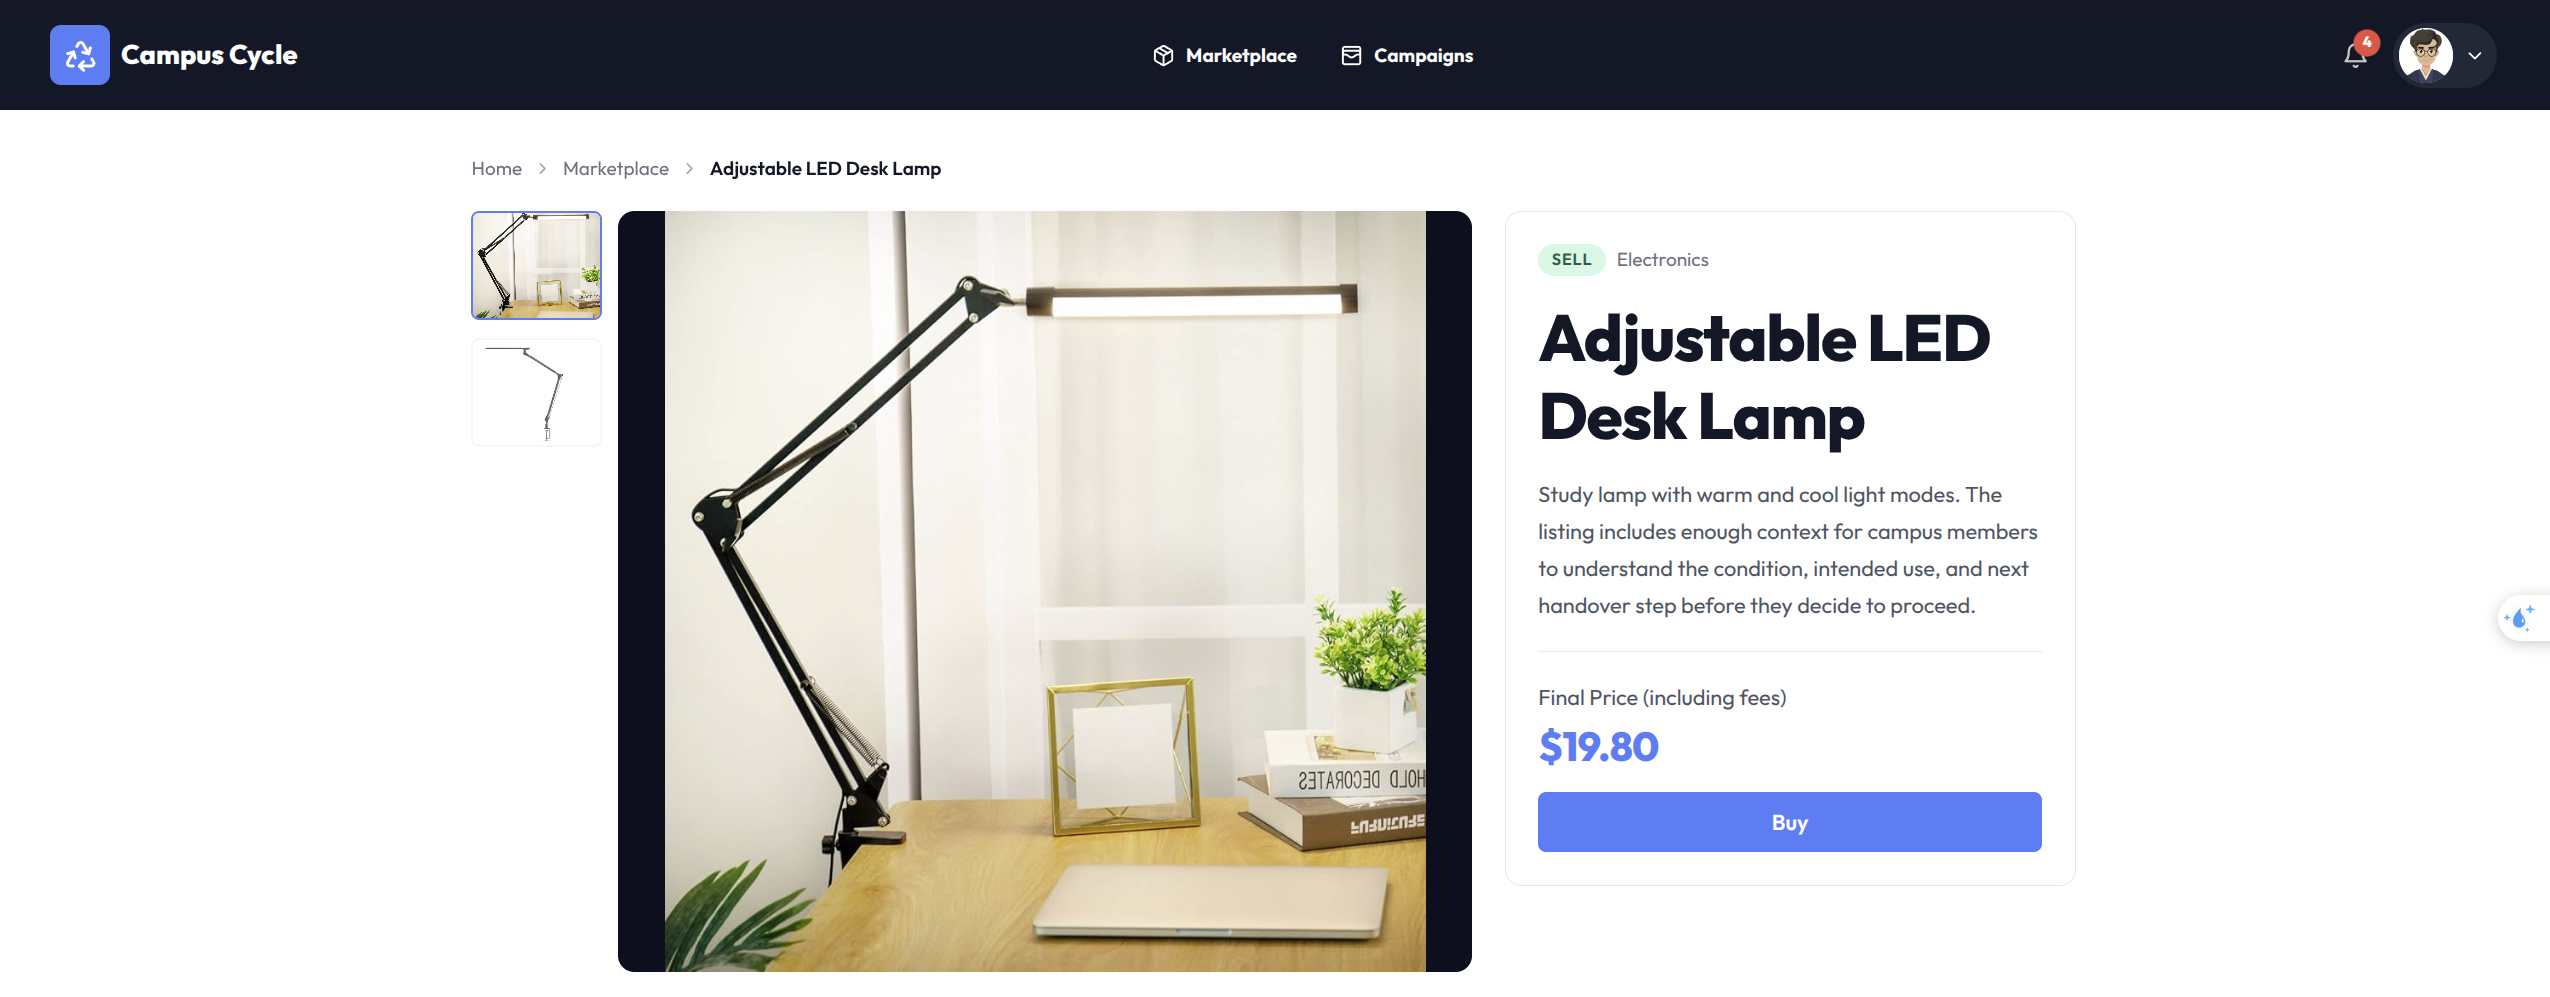
\includegraphics[width=0.75\textwidth]{Item Detail Page.png}
\caption{Item Detail Page}
\label{fig:item-detail-page}
\end{figure}

Checkout / Confirm Purchase Page: Cho phép member kiểm tra lại thông tin trước khi xác nhận mua item.

\begin{figure}[H]
\centering
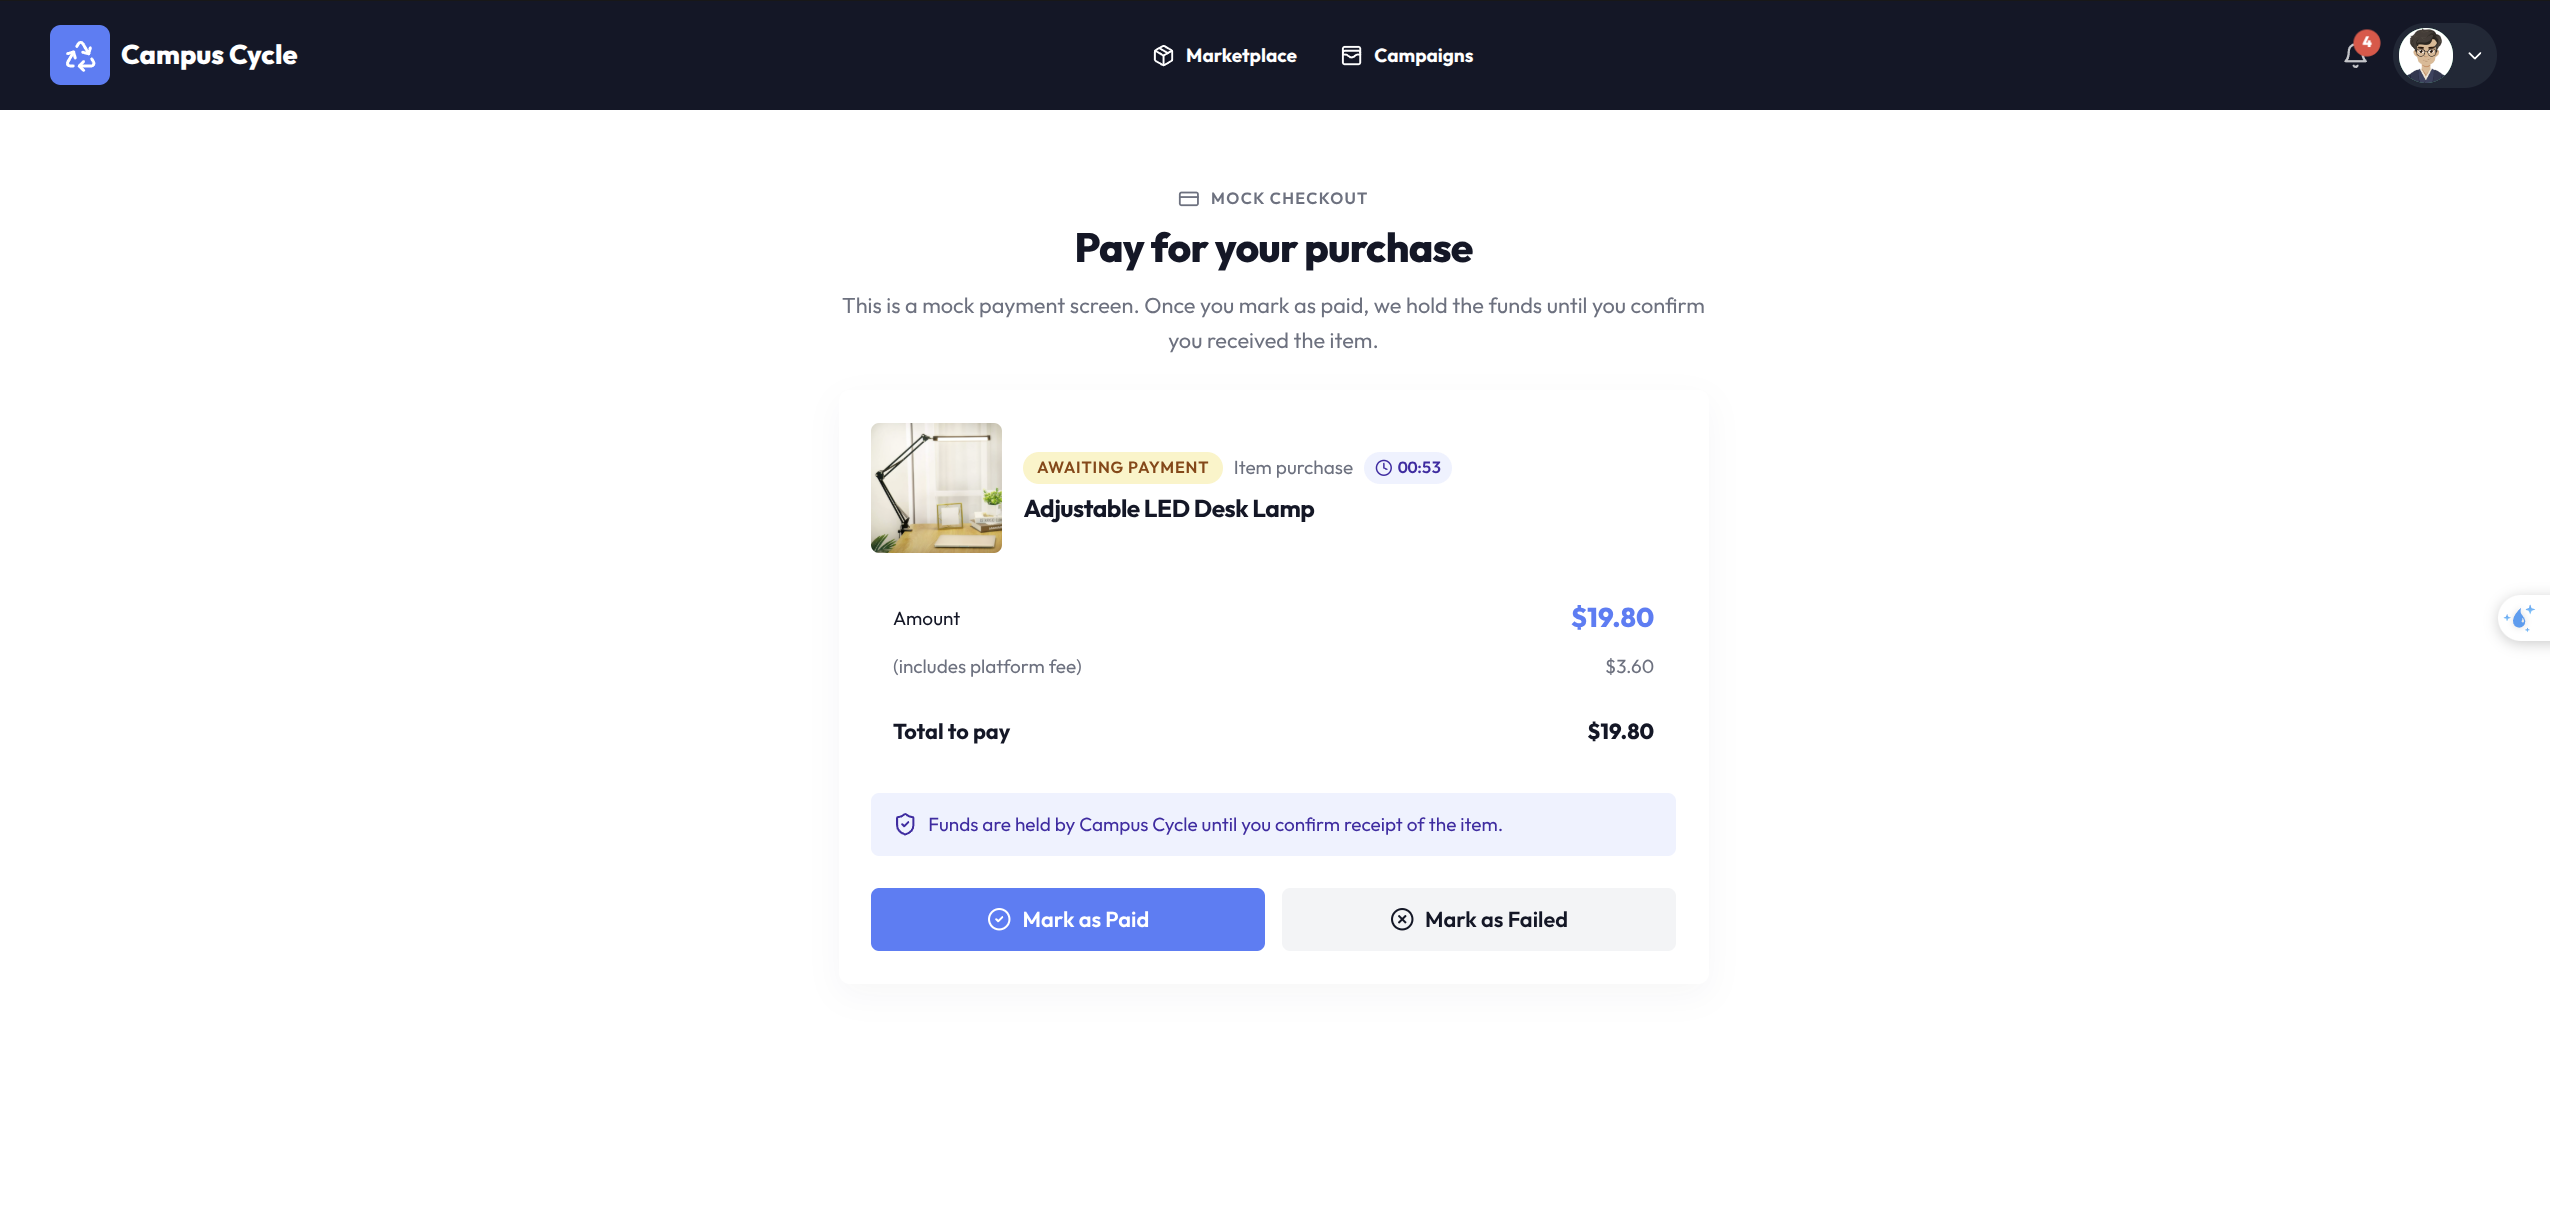
\includegraphics[width=0.75\textwidth]{Checkout.png}
\caption{Checkout / Confirm Purchase Page}
\label{fig:checkout-confirm-purchase-page}
\end{figure}

My Purchases Page: Hiển thị thông tin các giao dịch của member.

\begin{figure}[H]
\centering
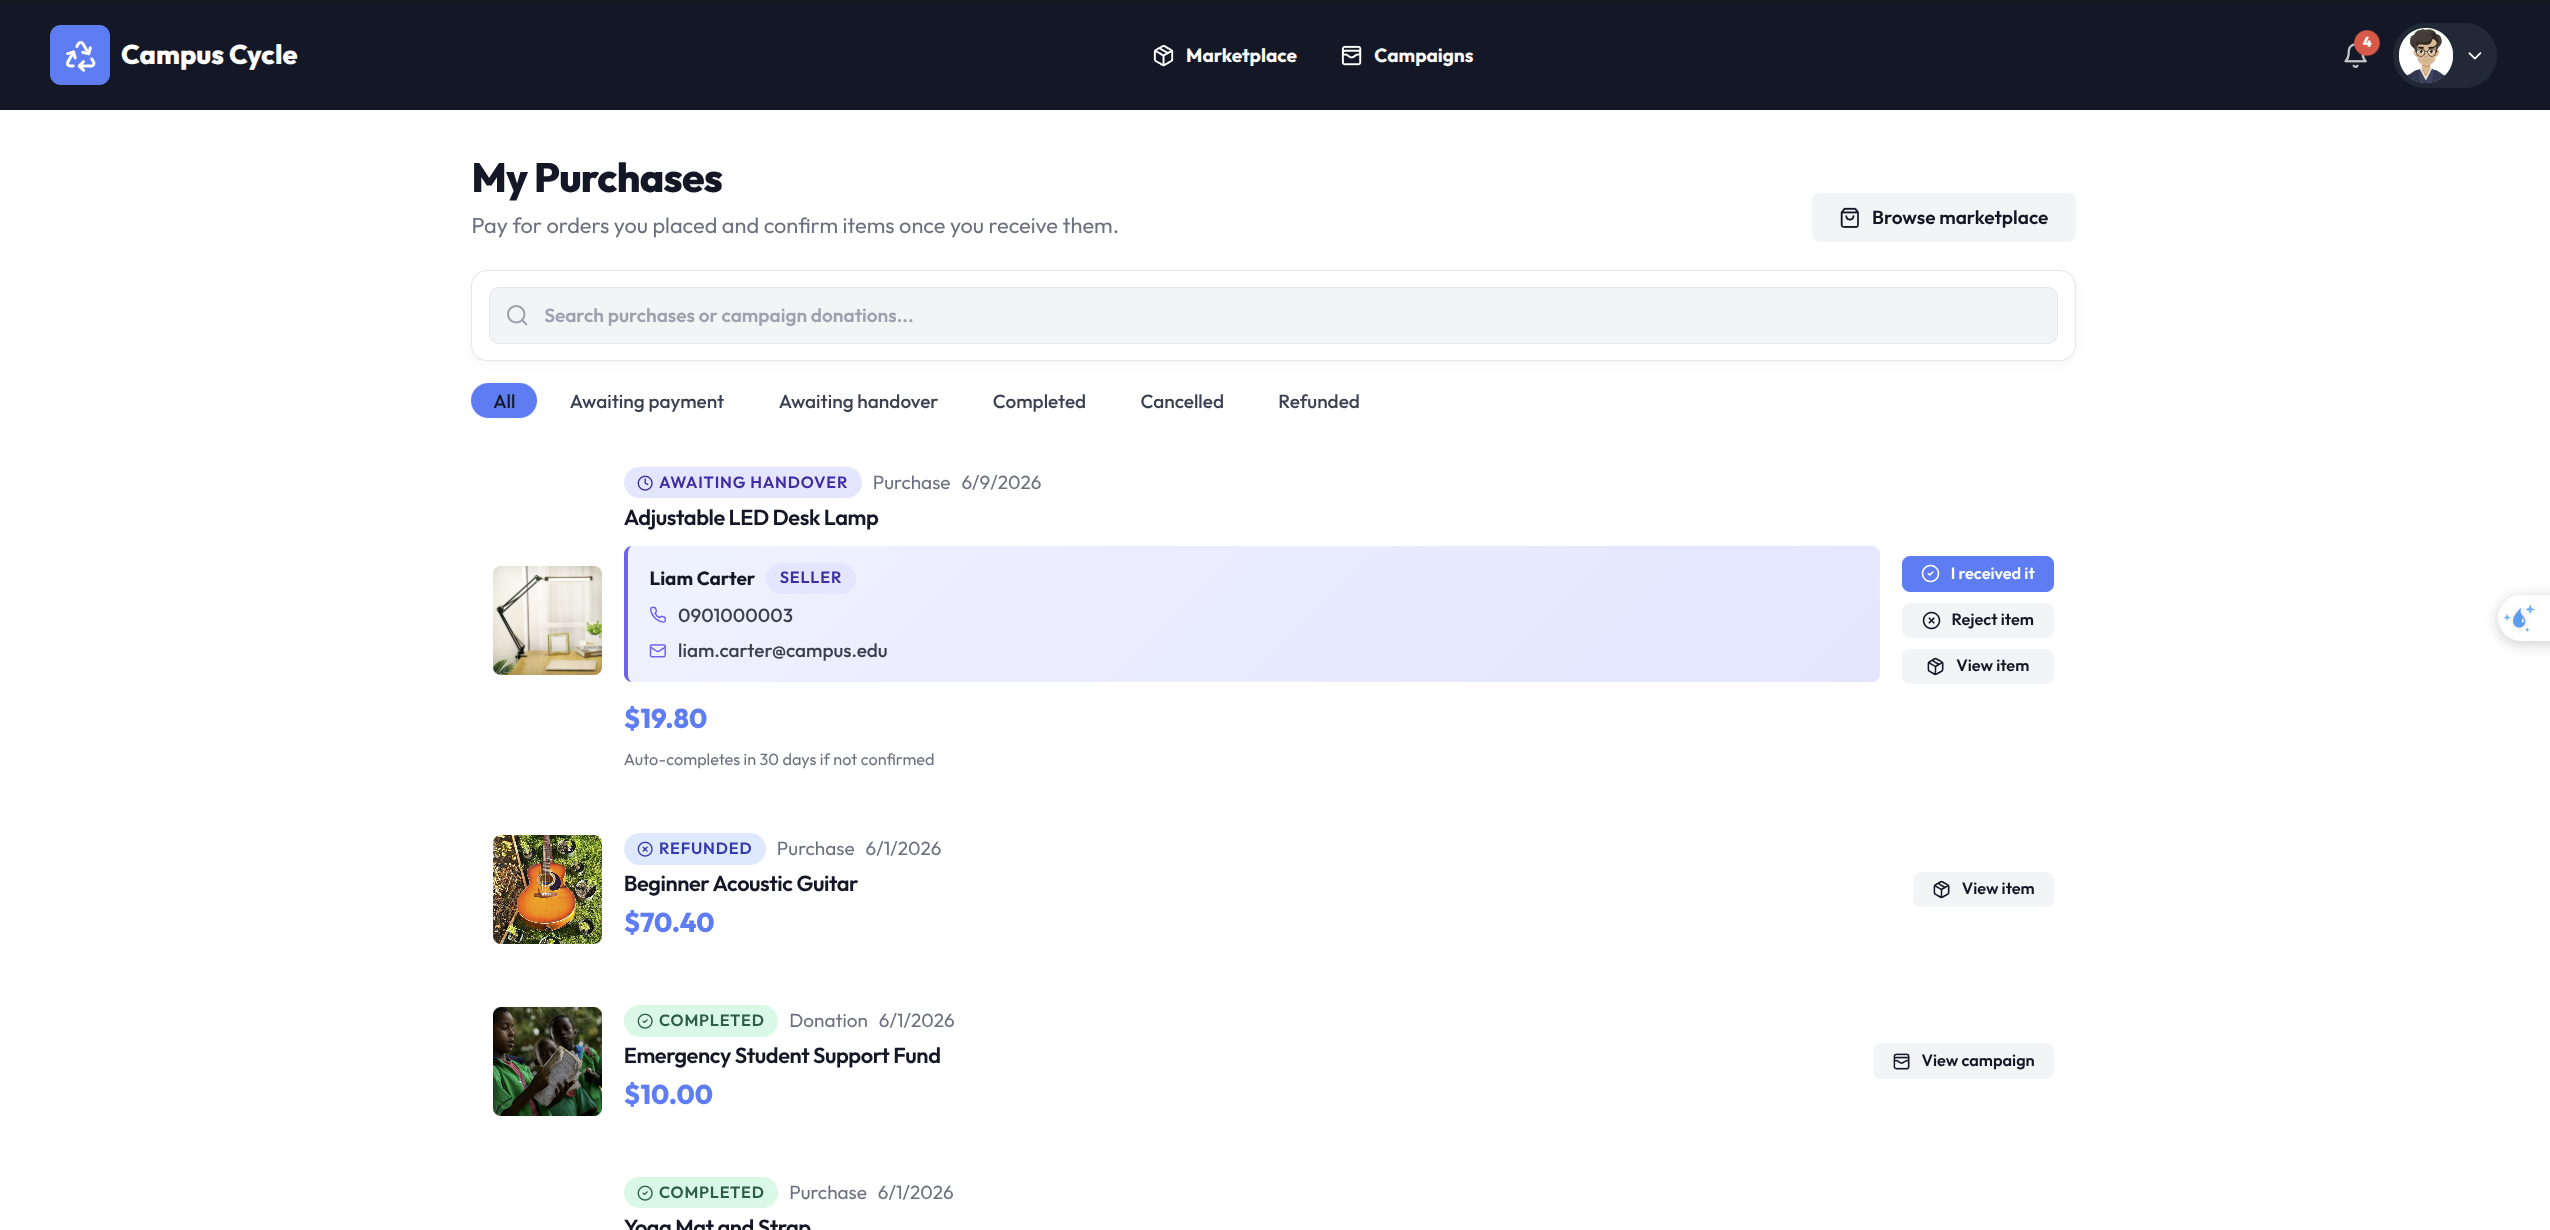
\includegraphics[width=0.75\textwidth]{My Purchases Page.png}
\caption{My Purchases Page}
\label{fig:my-purchases-page}
\end{figure}

Purchase Detail / Review Page: Cho phép member xem chi tiết đơn mua và thông tin người bán khi member đã thanh toán cho ứng dụng.

\begin{figure}[H]
\centering
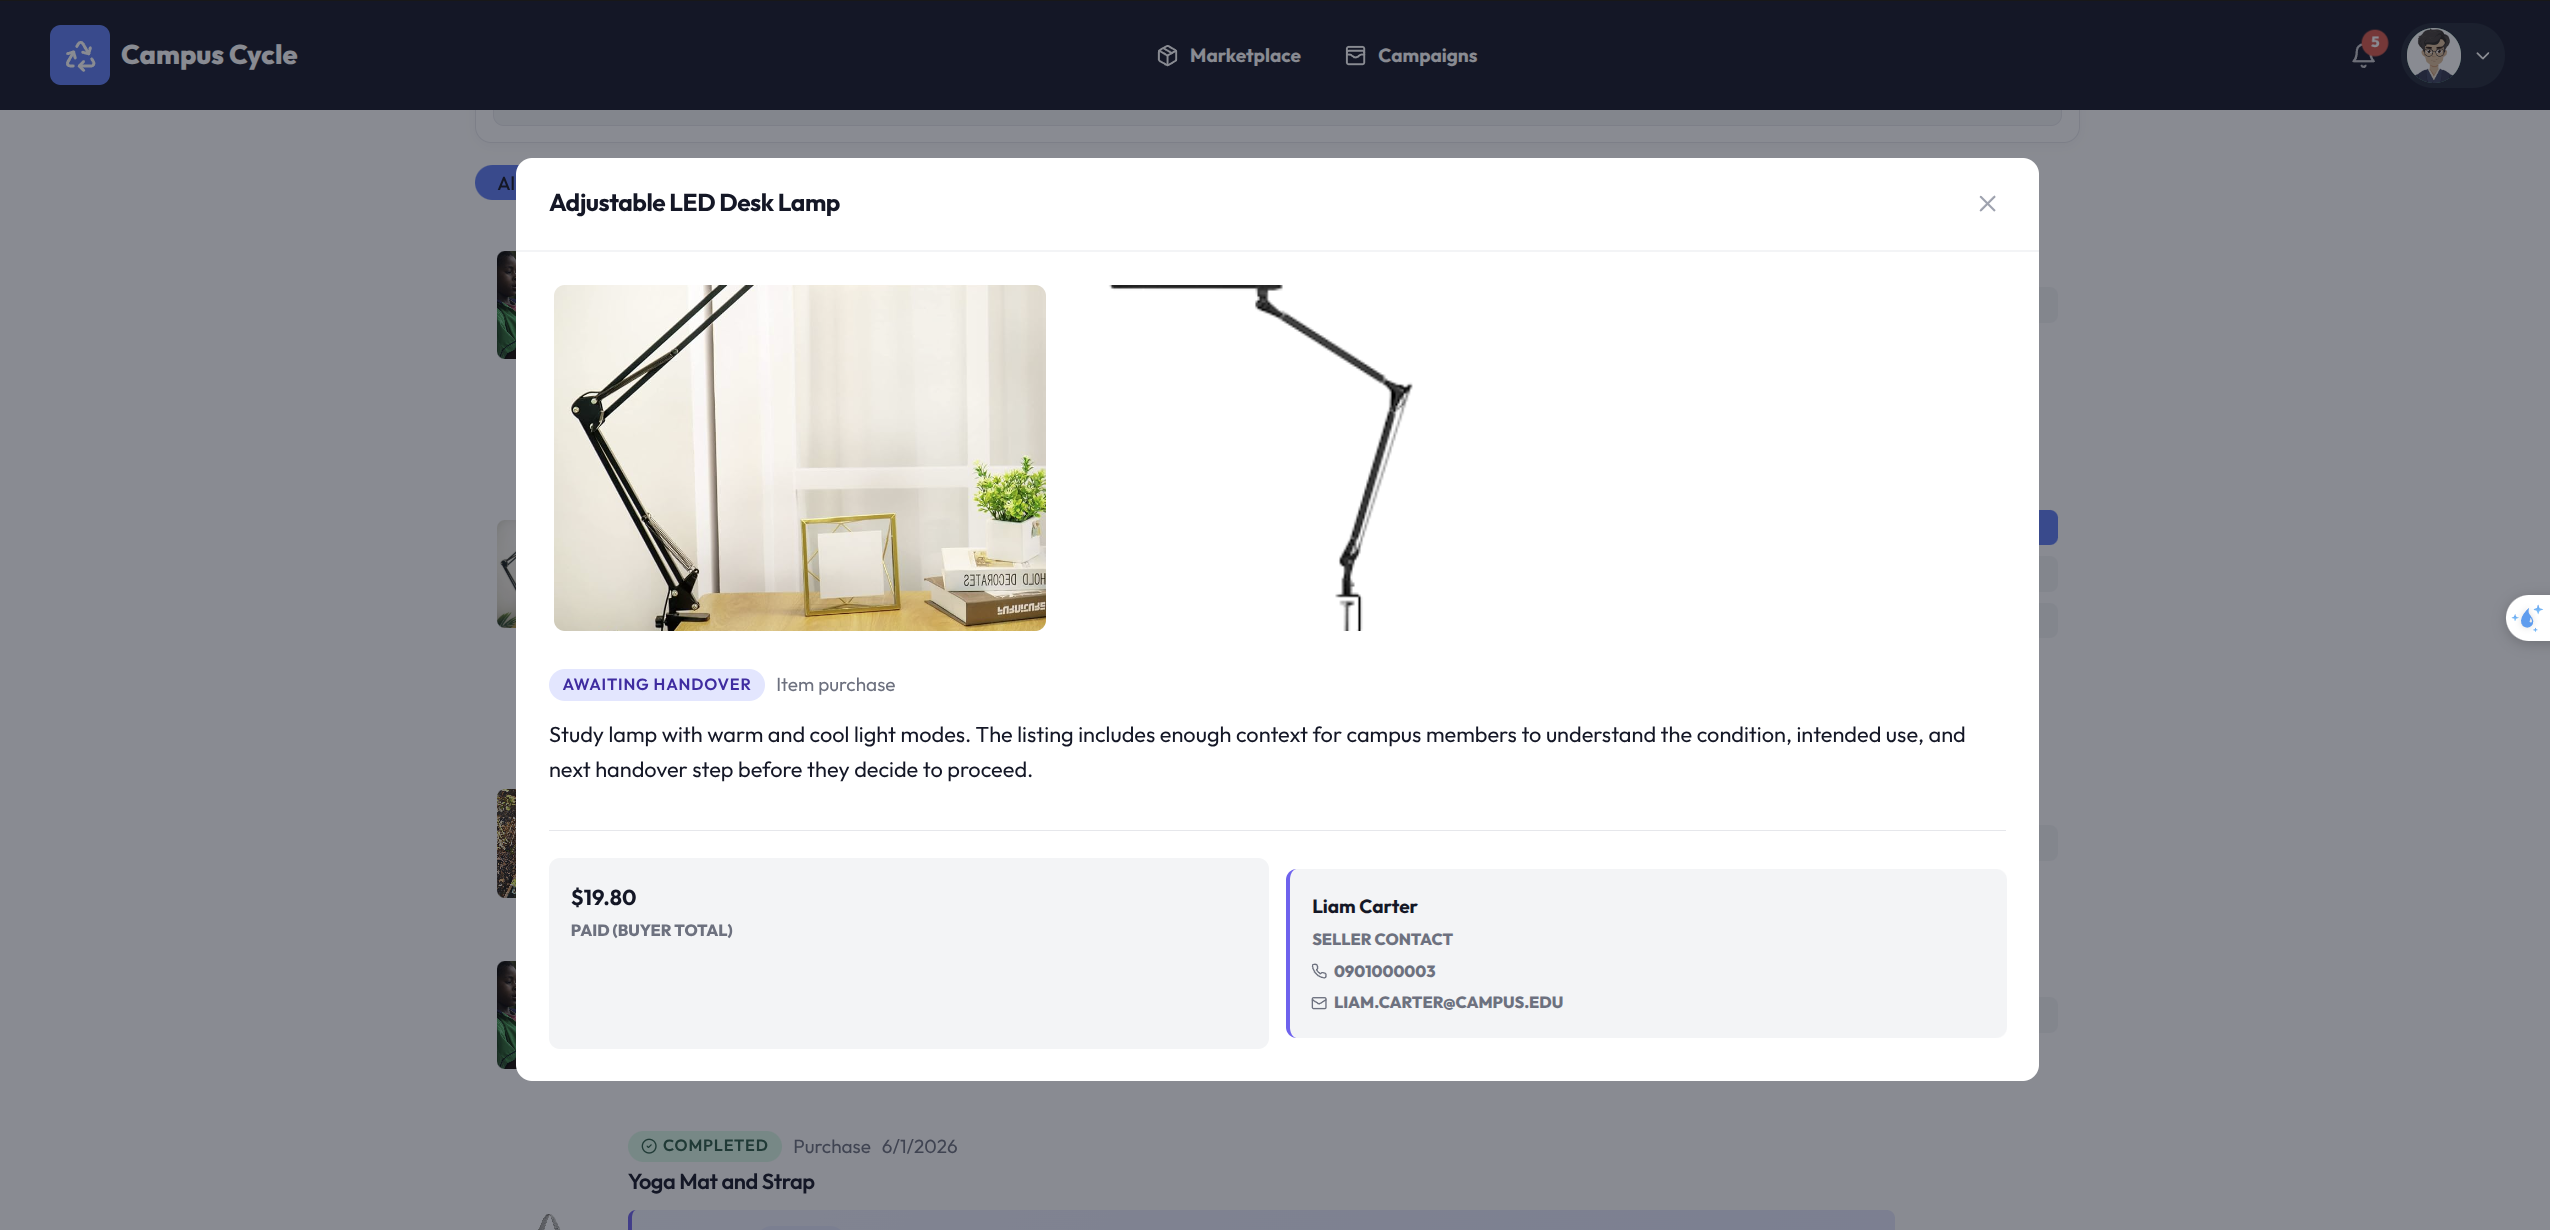
\includegraphics[width=0.75\textwidth]{Purchase dr Page.png}
\caption{Purchase Detail / Review Page}
\label{fig:purchase-detail-review-page}
\end{figure}

Sell Item Page: Cho phép member đăng item cần bán lên hệ thống.

\begin{figure}[H]
\centering
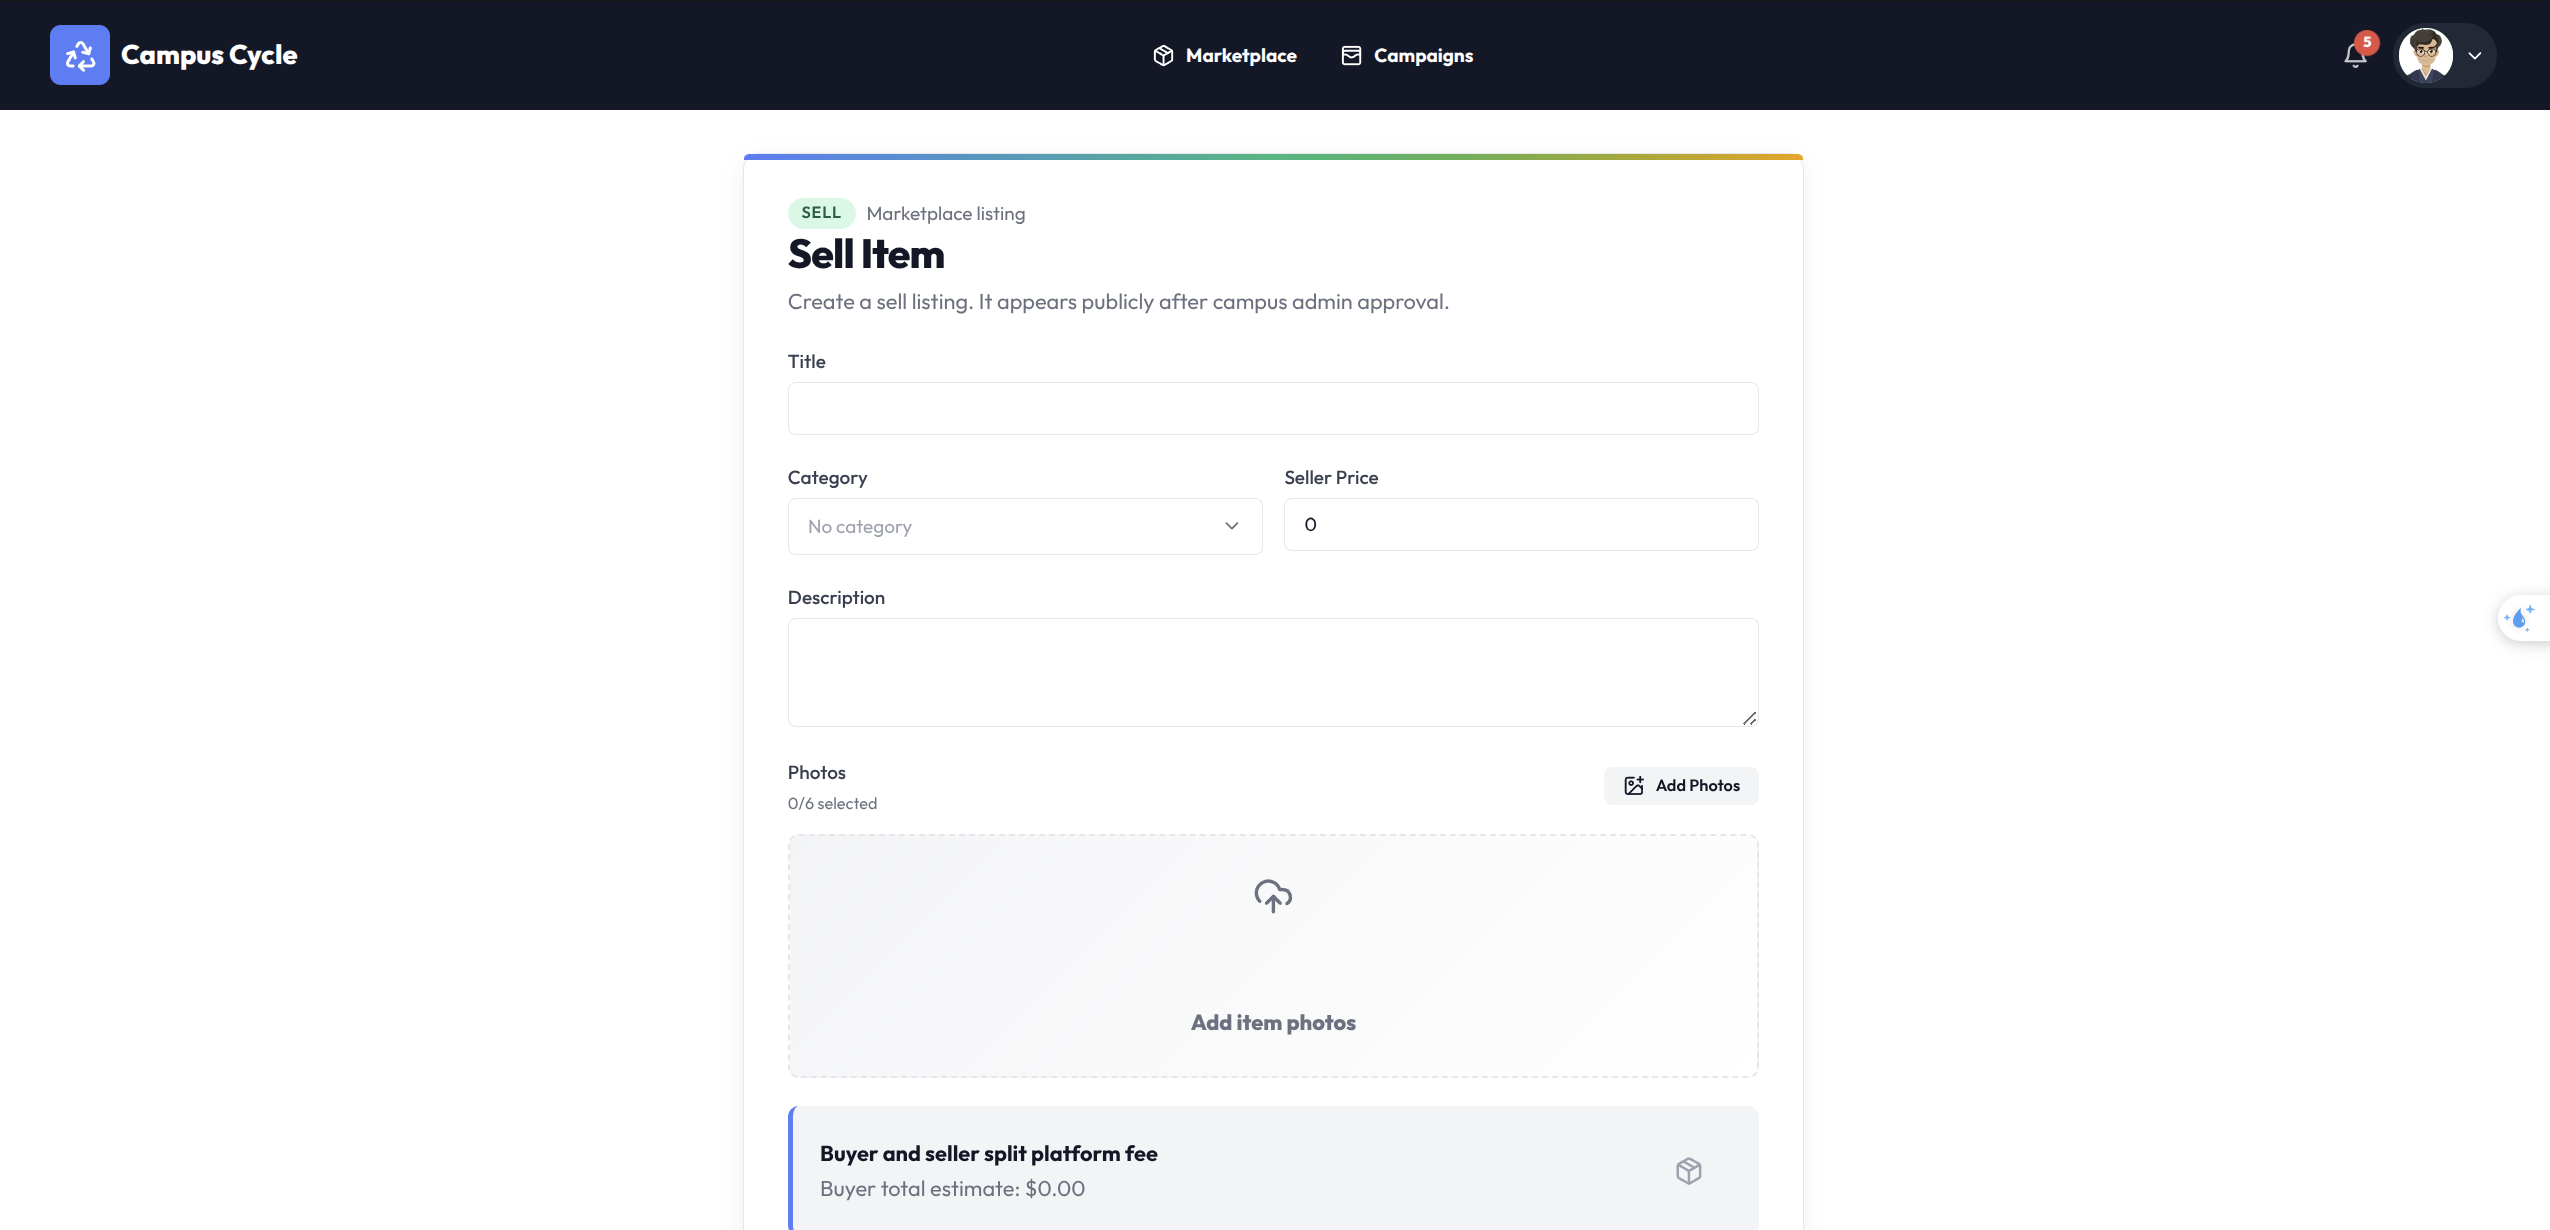
\includegraphics[width=0.75\textwidth]{Sell Item Page.png}
\caption{Sell Item Page}
\label{fig:sell-item-page}
\end{figure}

Donate Item Page: Cho phép member gửi item để quyên góp cho campaign.

\begin{figure}[H]
\centering
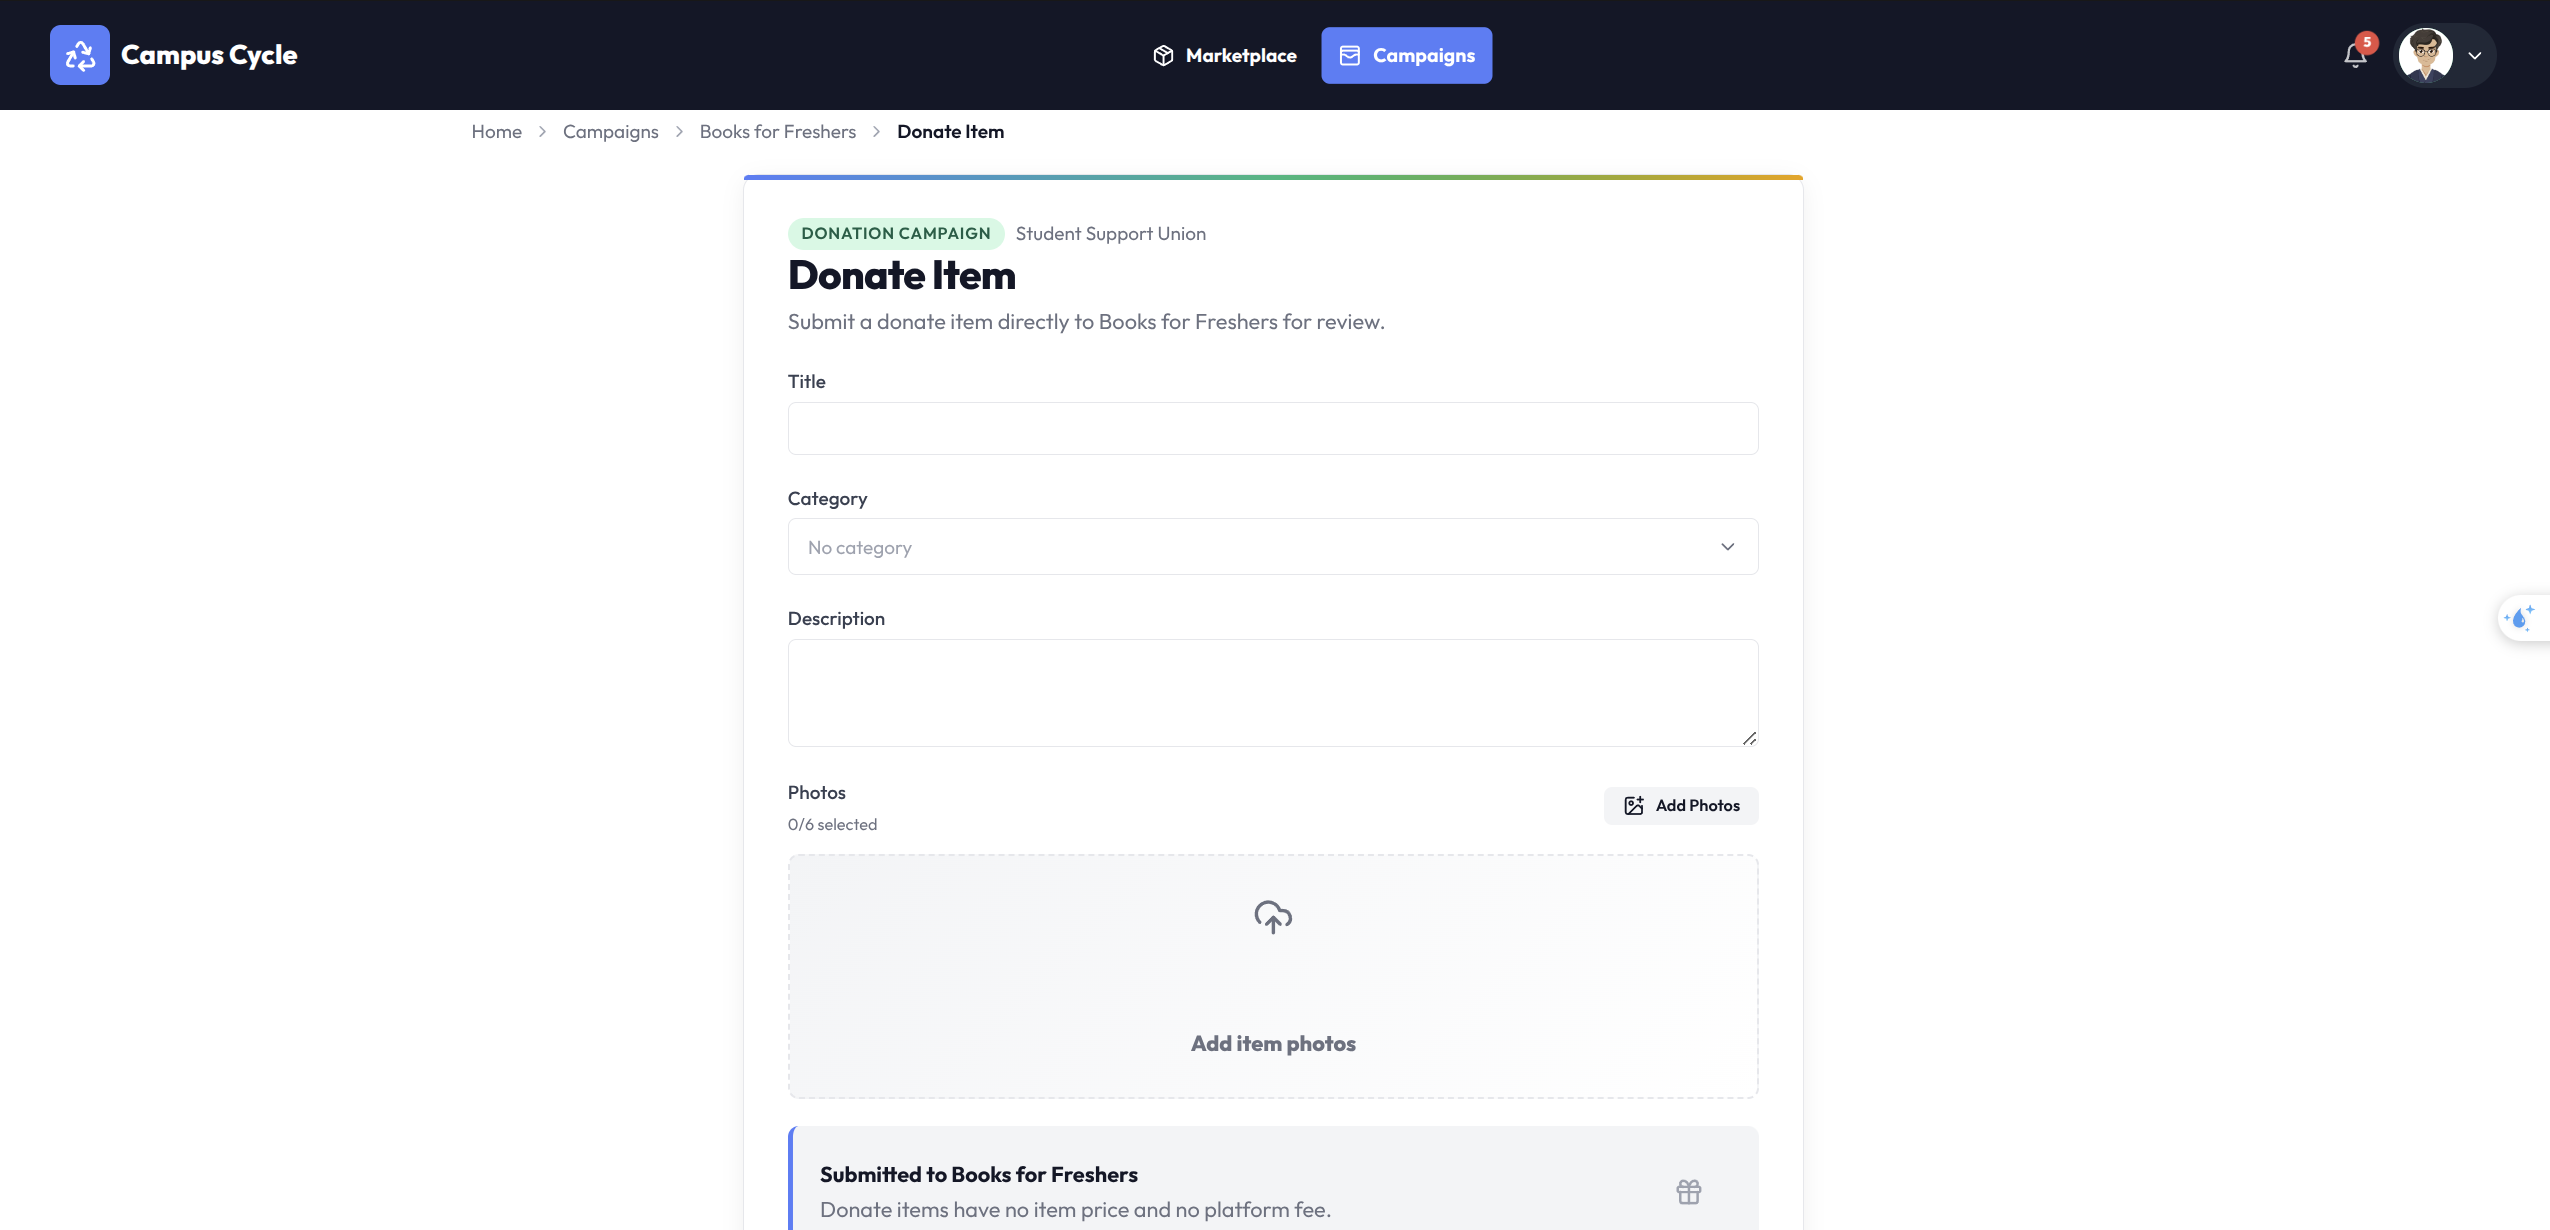
\includegraphics[width=0.75\textwidth]{Donate Item Page.png}
\caption{Donate Item Page}
\label{fig:donate-item-page}
\end{figure}

Donation Campaign Detail Page: Hiển thị thông tin chi tiết của một donation campaign.

\begin{figure}[H]
\centering
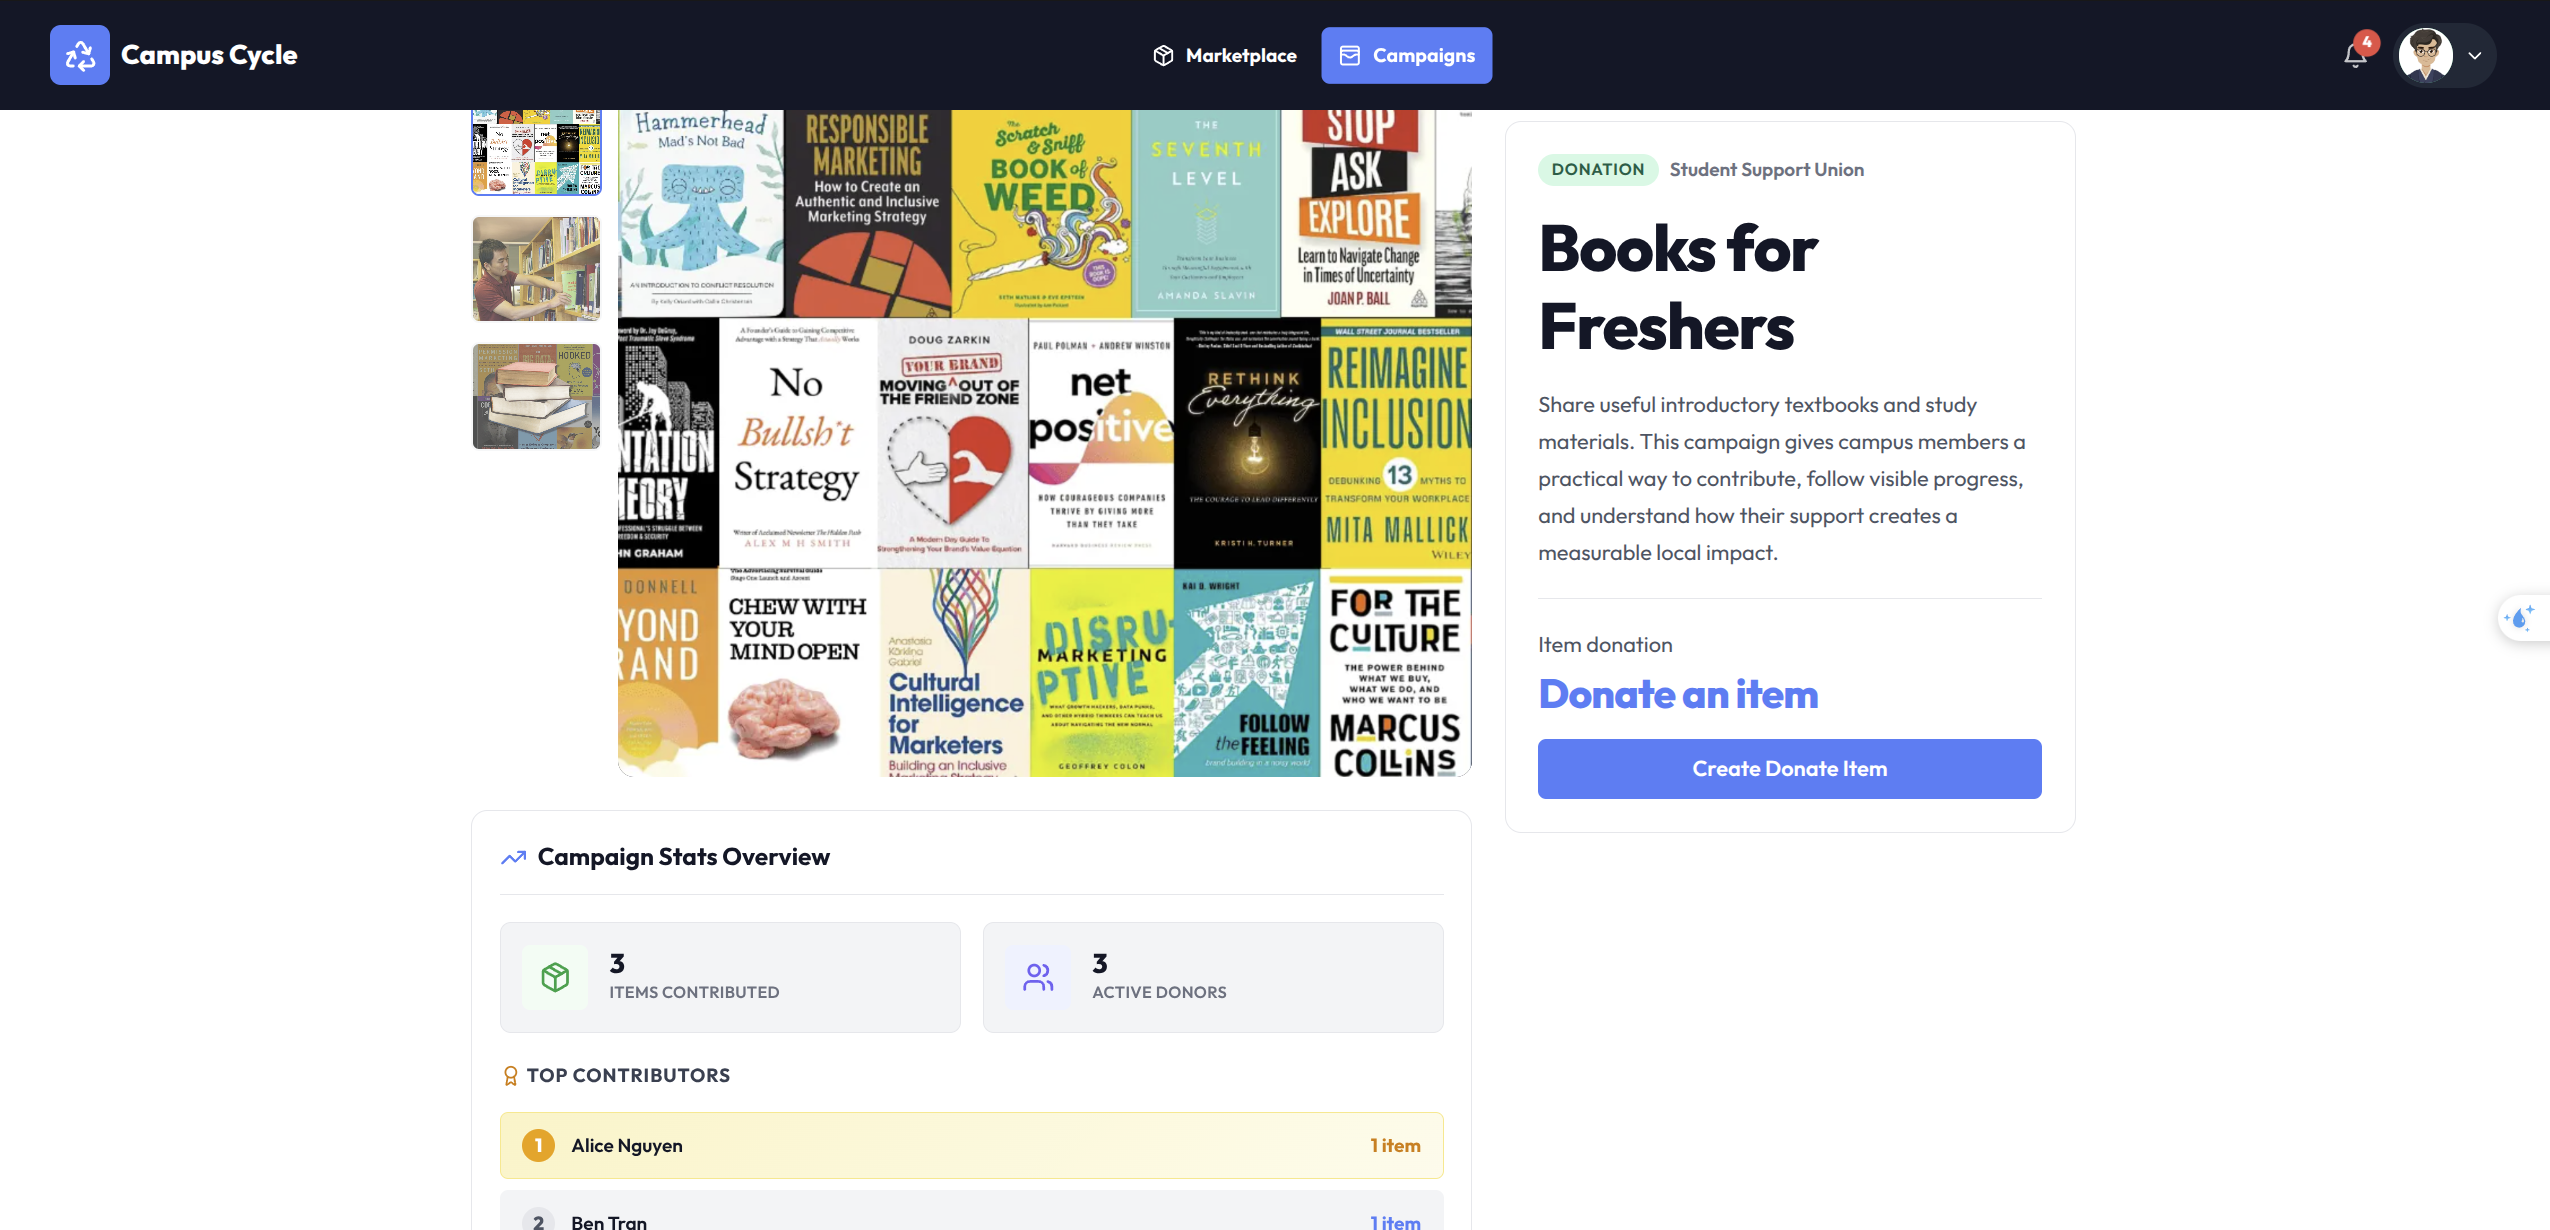
\includegraphics[width=0.75\textwidth]{Campaign Detail Pagemb.png}
\caption{Donation Campaign Detail Page}
\label{fig:campaign-detail-member-page}
\end{figure}

Fundraising Campaign Detail Page: Hiển thị thông tin chi tiết của một Fundraising campaign.

\begin{figure}[H]
\centering
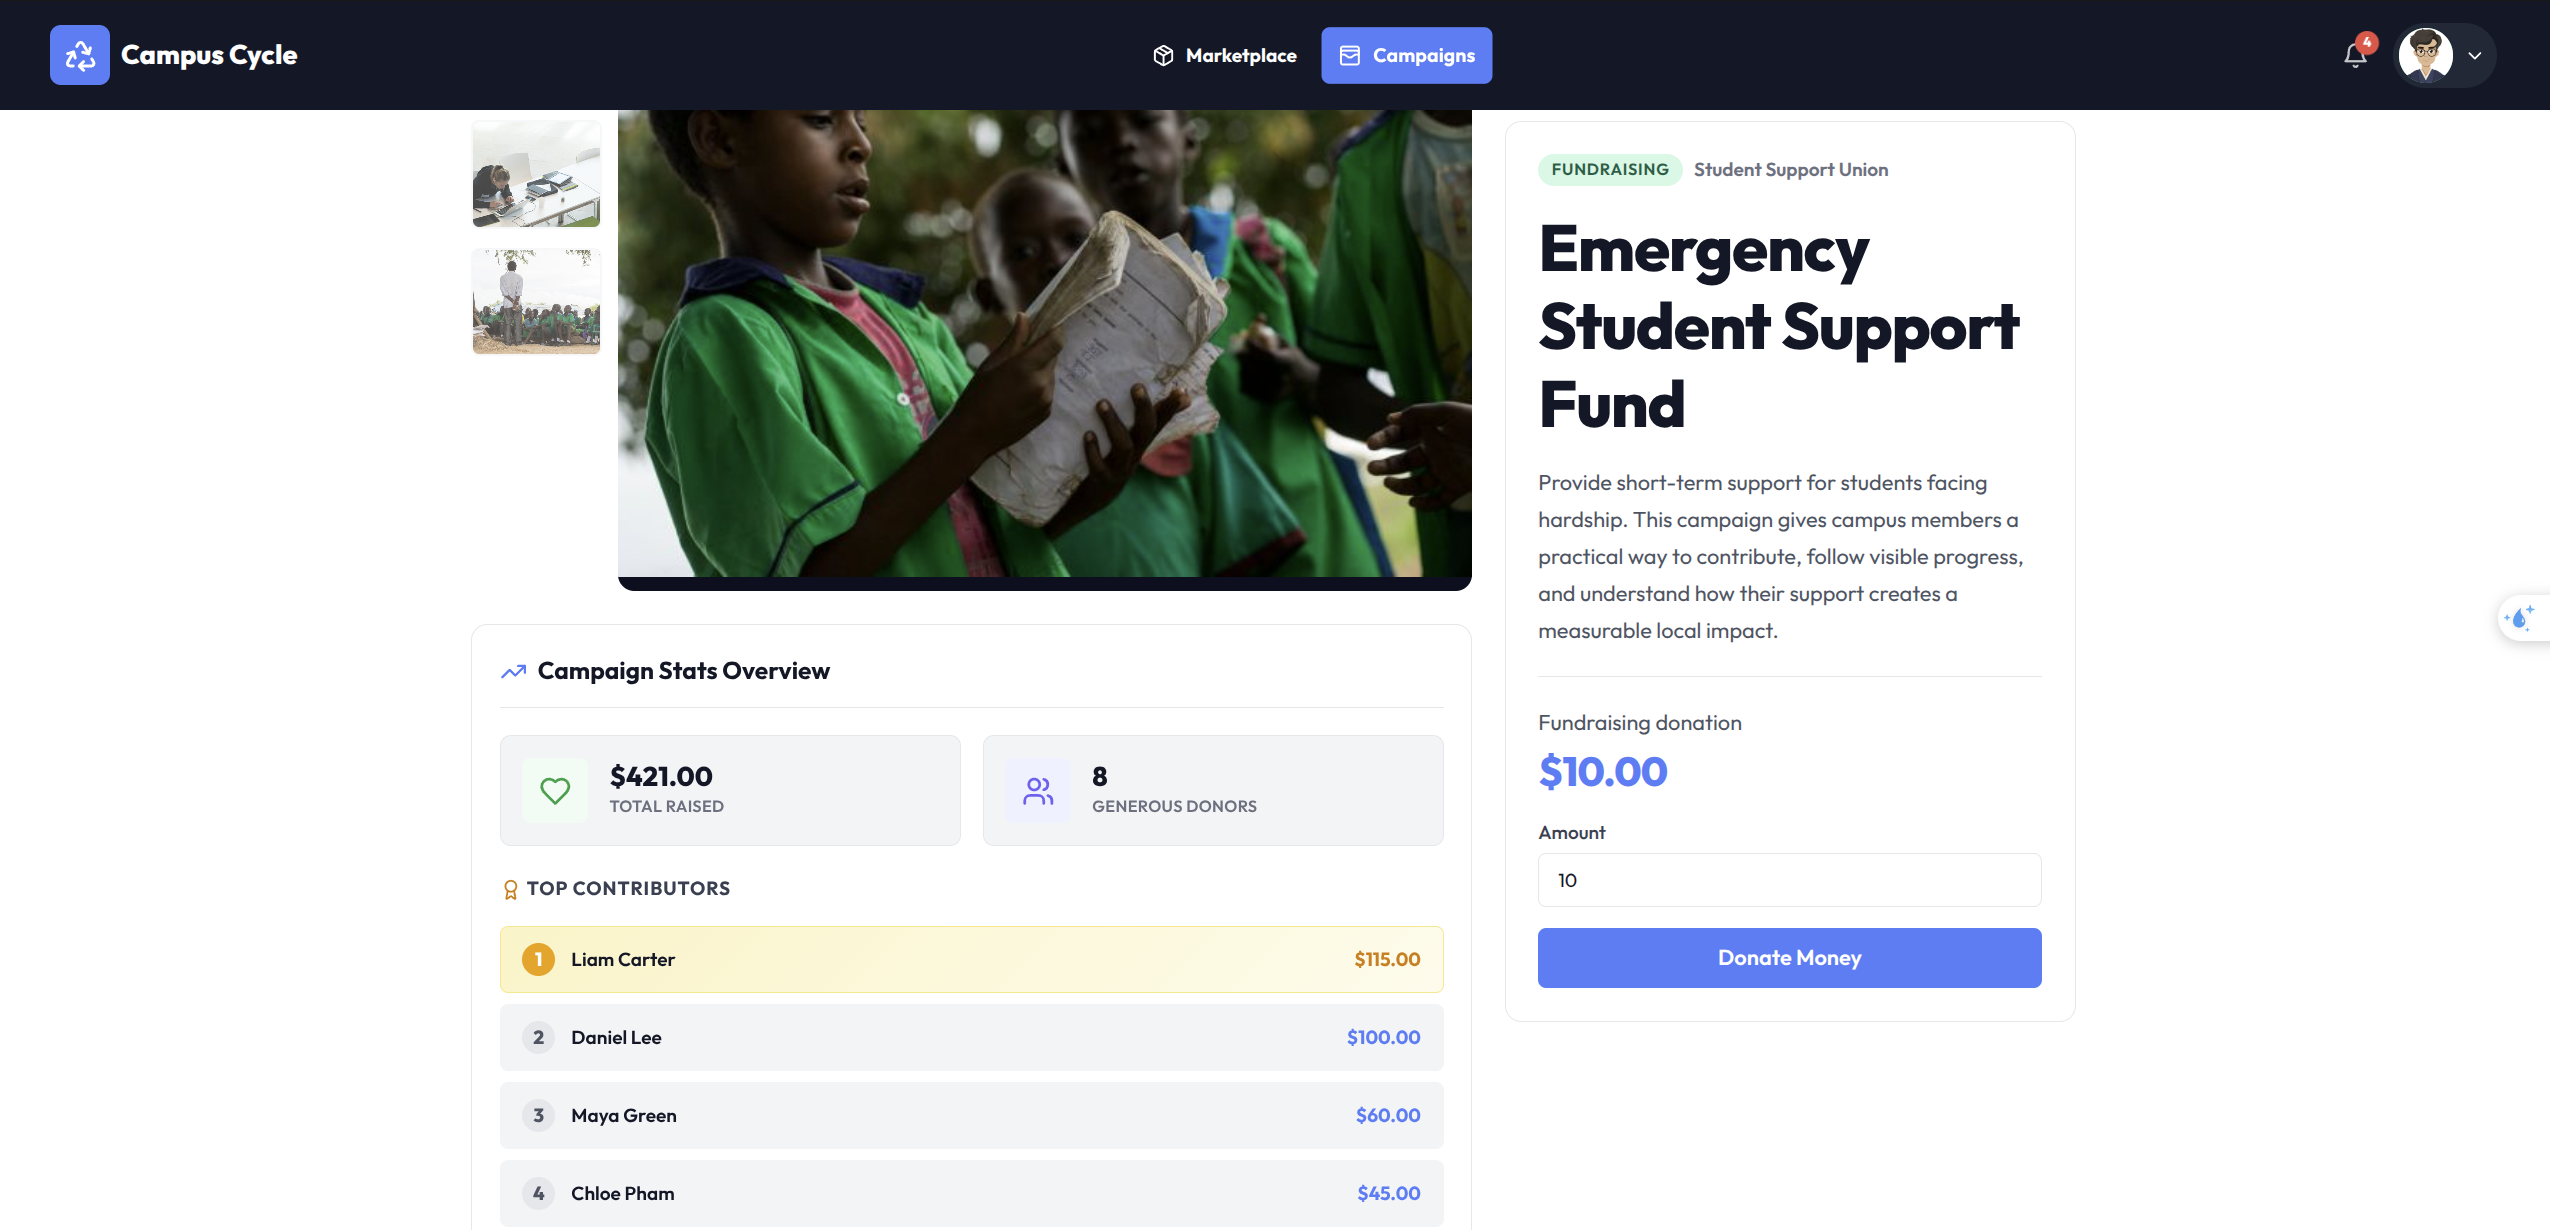
\includegraphics[width=0.75\textwidth]{Donation Page.png}
\caption{Fundraising Campaign Detail Page}
\label{fig:donation-page}
\end{figure}

My Items Page: Hiển thị các item do member đã đăng lên hệ thống.

\begin{figure}[H]
\centering
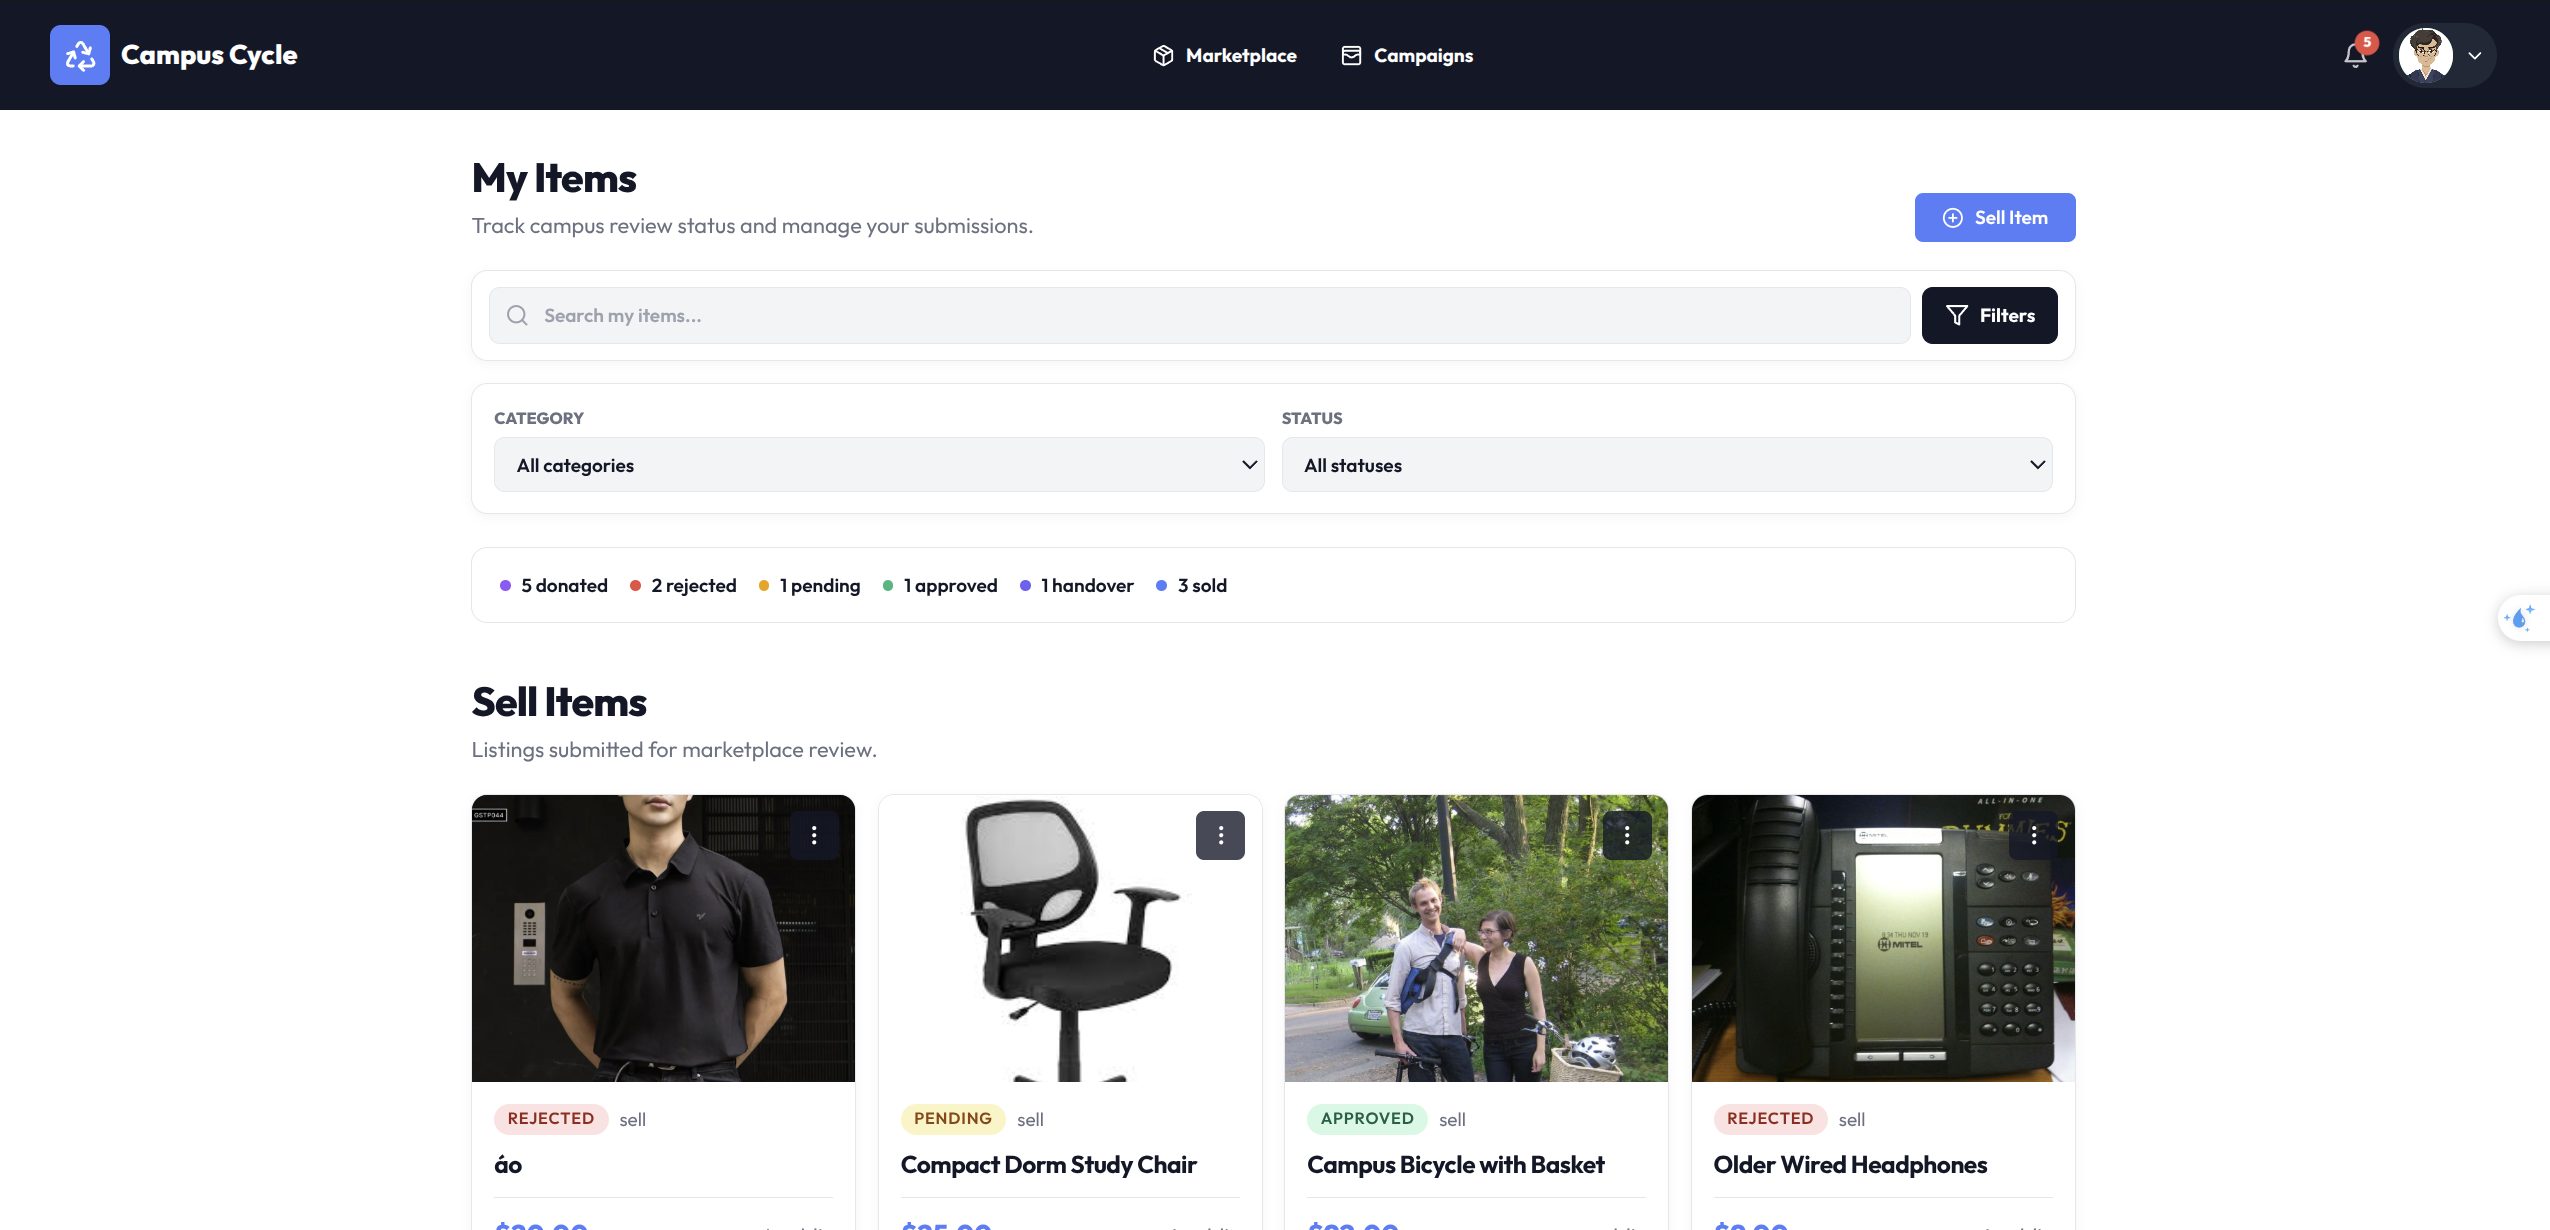
\includegraphics[width=0.75\textwidth]{My Items Page.png}
\caption{My Items Page}
\label{fig:my-items-page}
\end{figure}

Profile Page: Cho phép member xem và cập nhật thông tin cá nhân.

\begin{figure}[H]
\centering
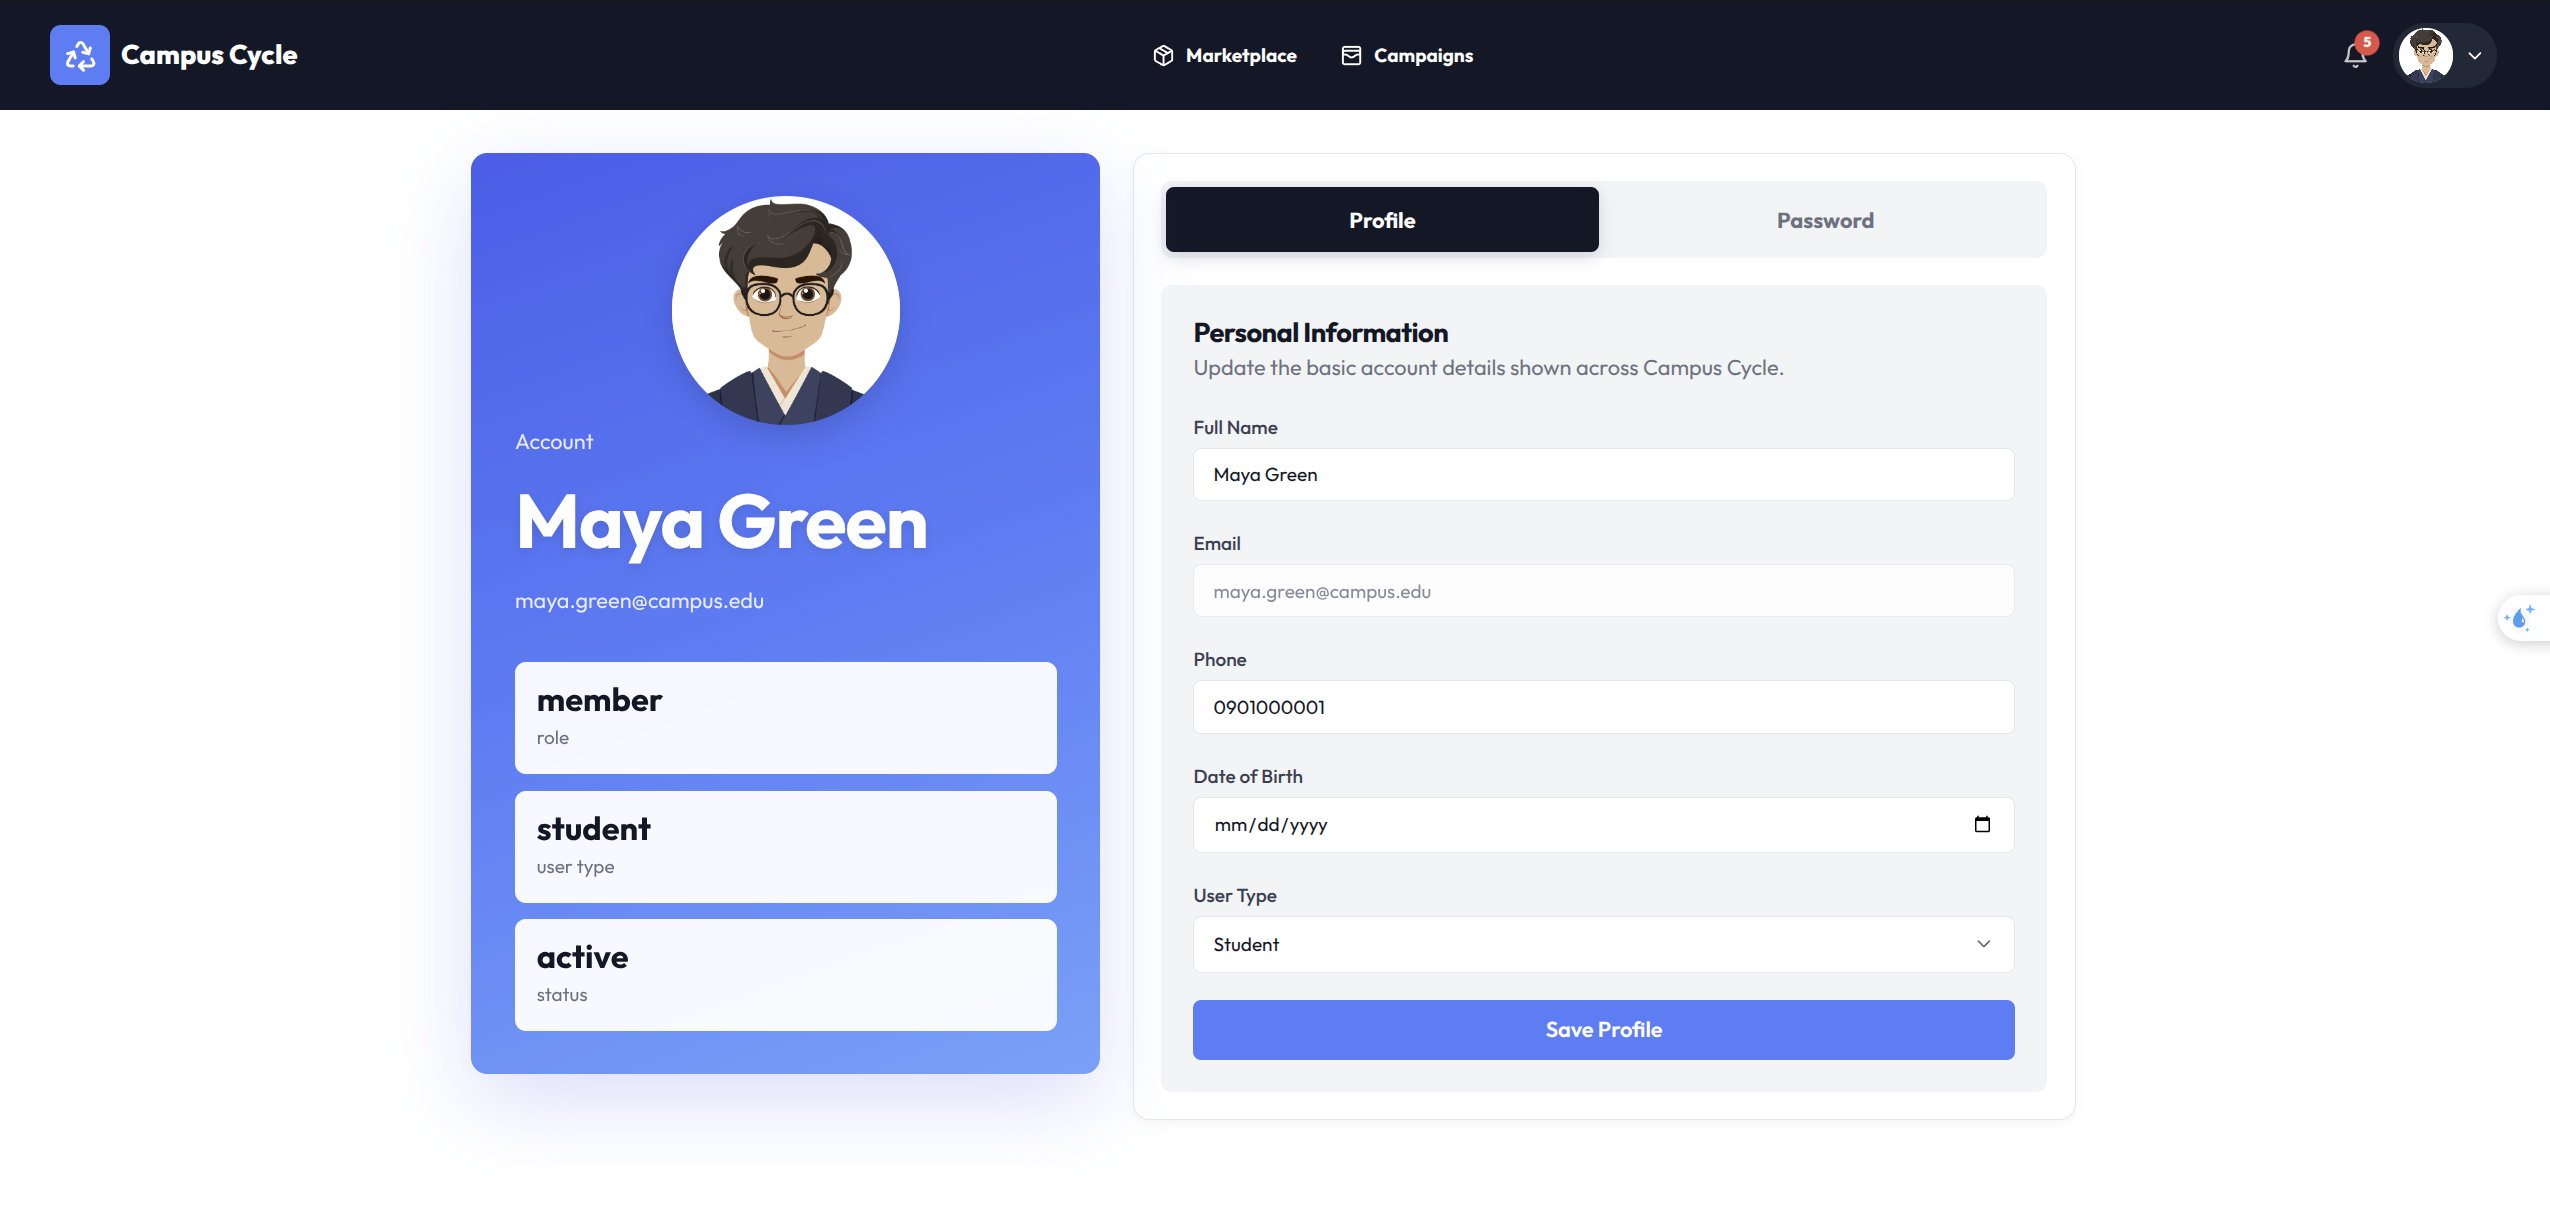
\includegraphics[width=0.75\textwidth]{Profile Page.png}
\caption{Profile Page}
\label{fig:profile-page}
\end{figure}

\subsection{Nhóm giao diện quản trị tổ chức}

Nhóm giao diện này dành cho Organization Admin, là người phụ trách quản lý các chiến dịch gây quỹ của tổ chức. Organization Admin có thể theo dõi dashboard, tạo và quản lý campaign, xem danh sách donated items, duyệt hoặc từ chối vật phẩm, đồng thời theo dõi hiệu quả của từng campaign.

Organization Dashboard: Hiển thị statistics tổng quan về campaign, donation và donated items.

\begin{figure}[H]
\centering
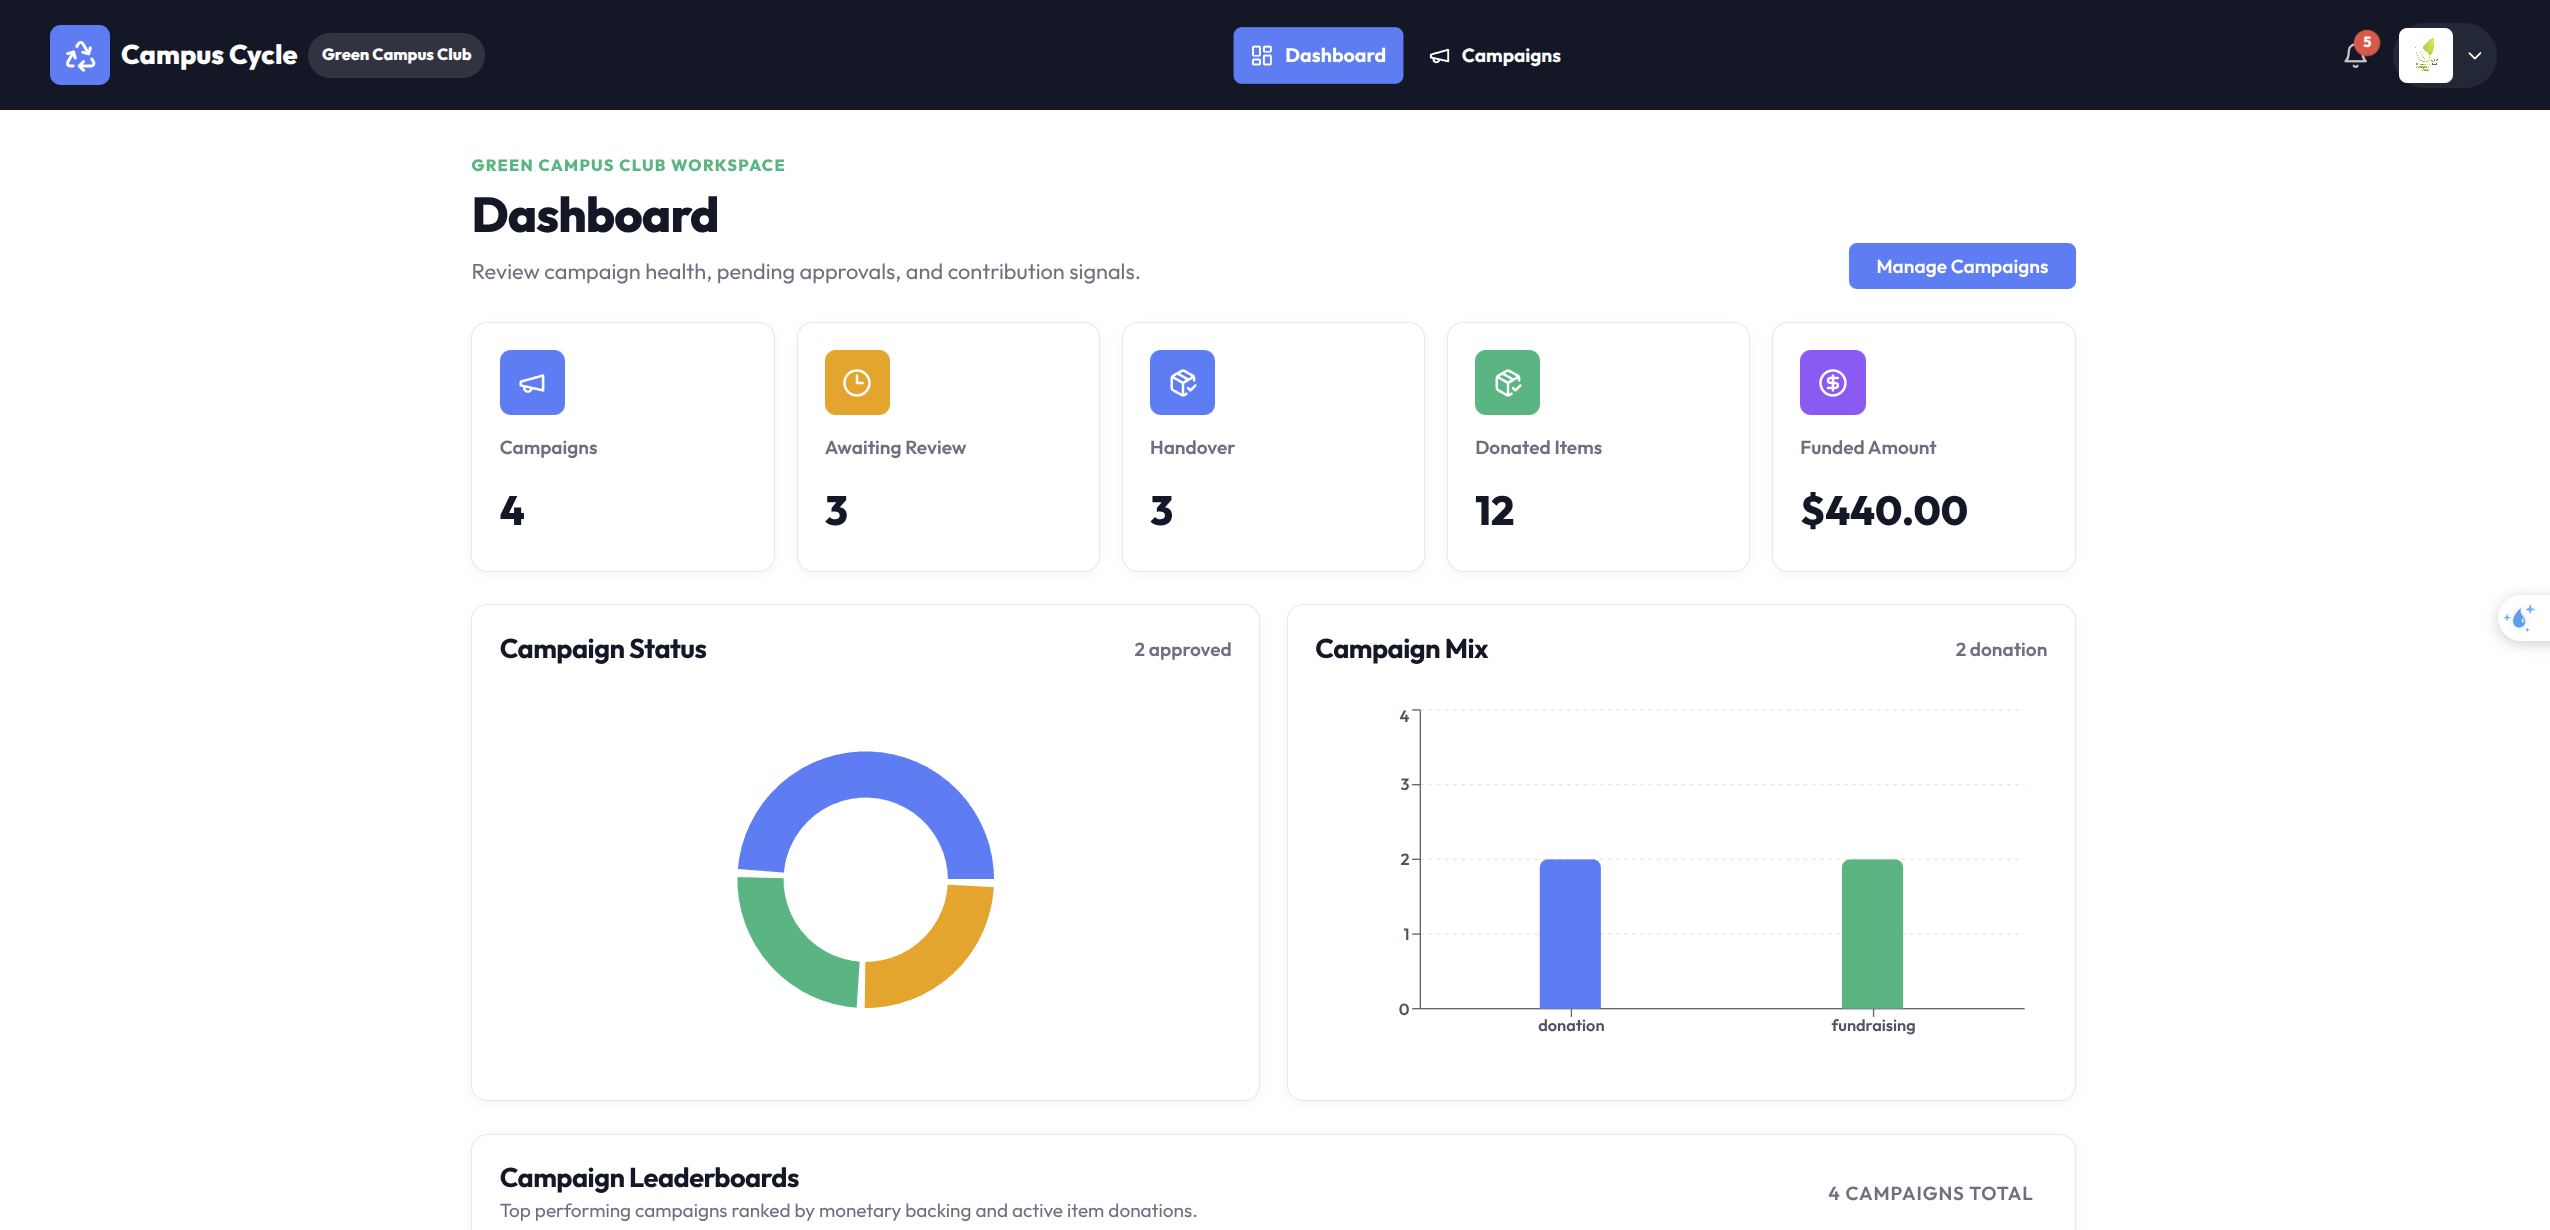
\includegraphics[width=0.75\textwidth]{Organization Dashboard.png}
\caption{Organization Dashboard}
\label{fig:organization-dashboard}
\end{figure}

Campaign Management Page: Hiển thị danh sách các campaign mà tổ chức đang quản lý.

\begin{figure}[H]
\centering
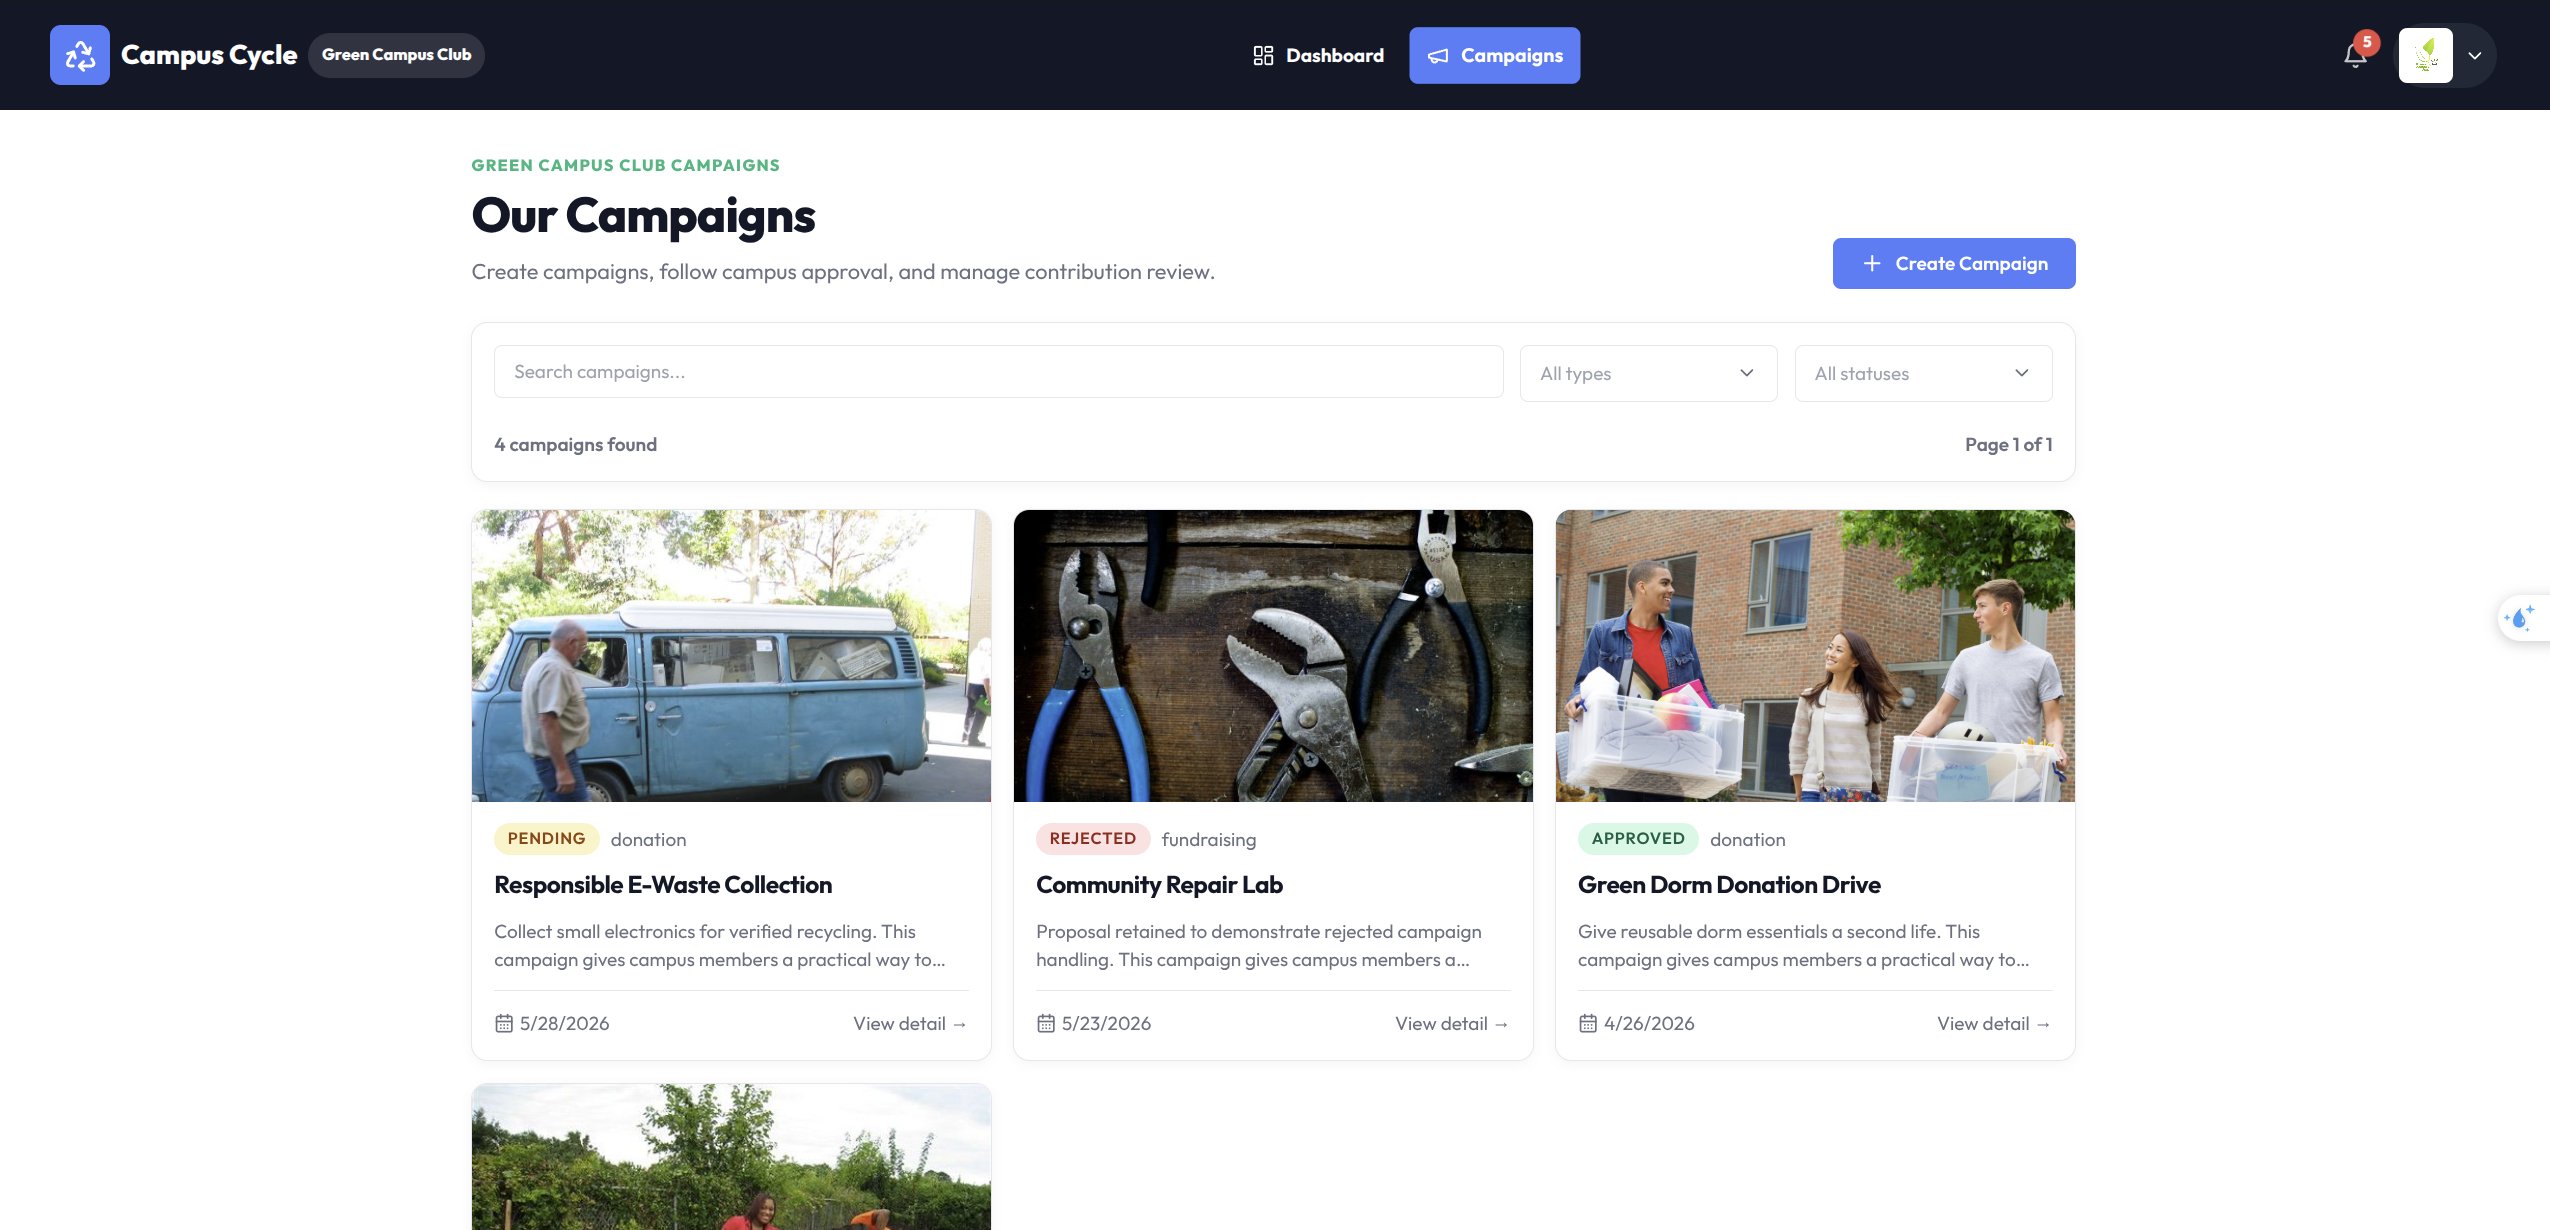
\includegraphics[width=0.75\textwidth]{Campaign Management Pageorg.png}
\caption{Campaign Management Page}
\label{fig:campaign-management-org-page}
\end{figure}

Campaign Detail Page: Hiển thị thông tin của một campaign.

\begin{figure}[H]
\centering
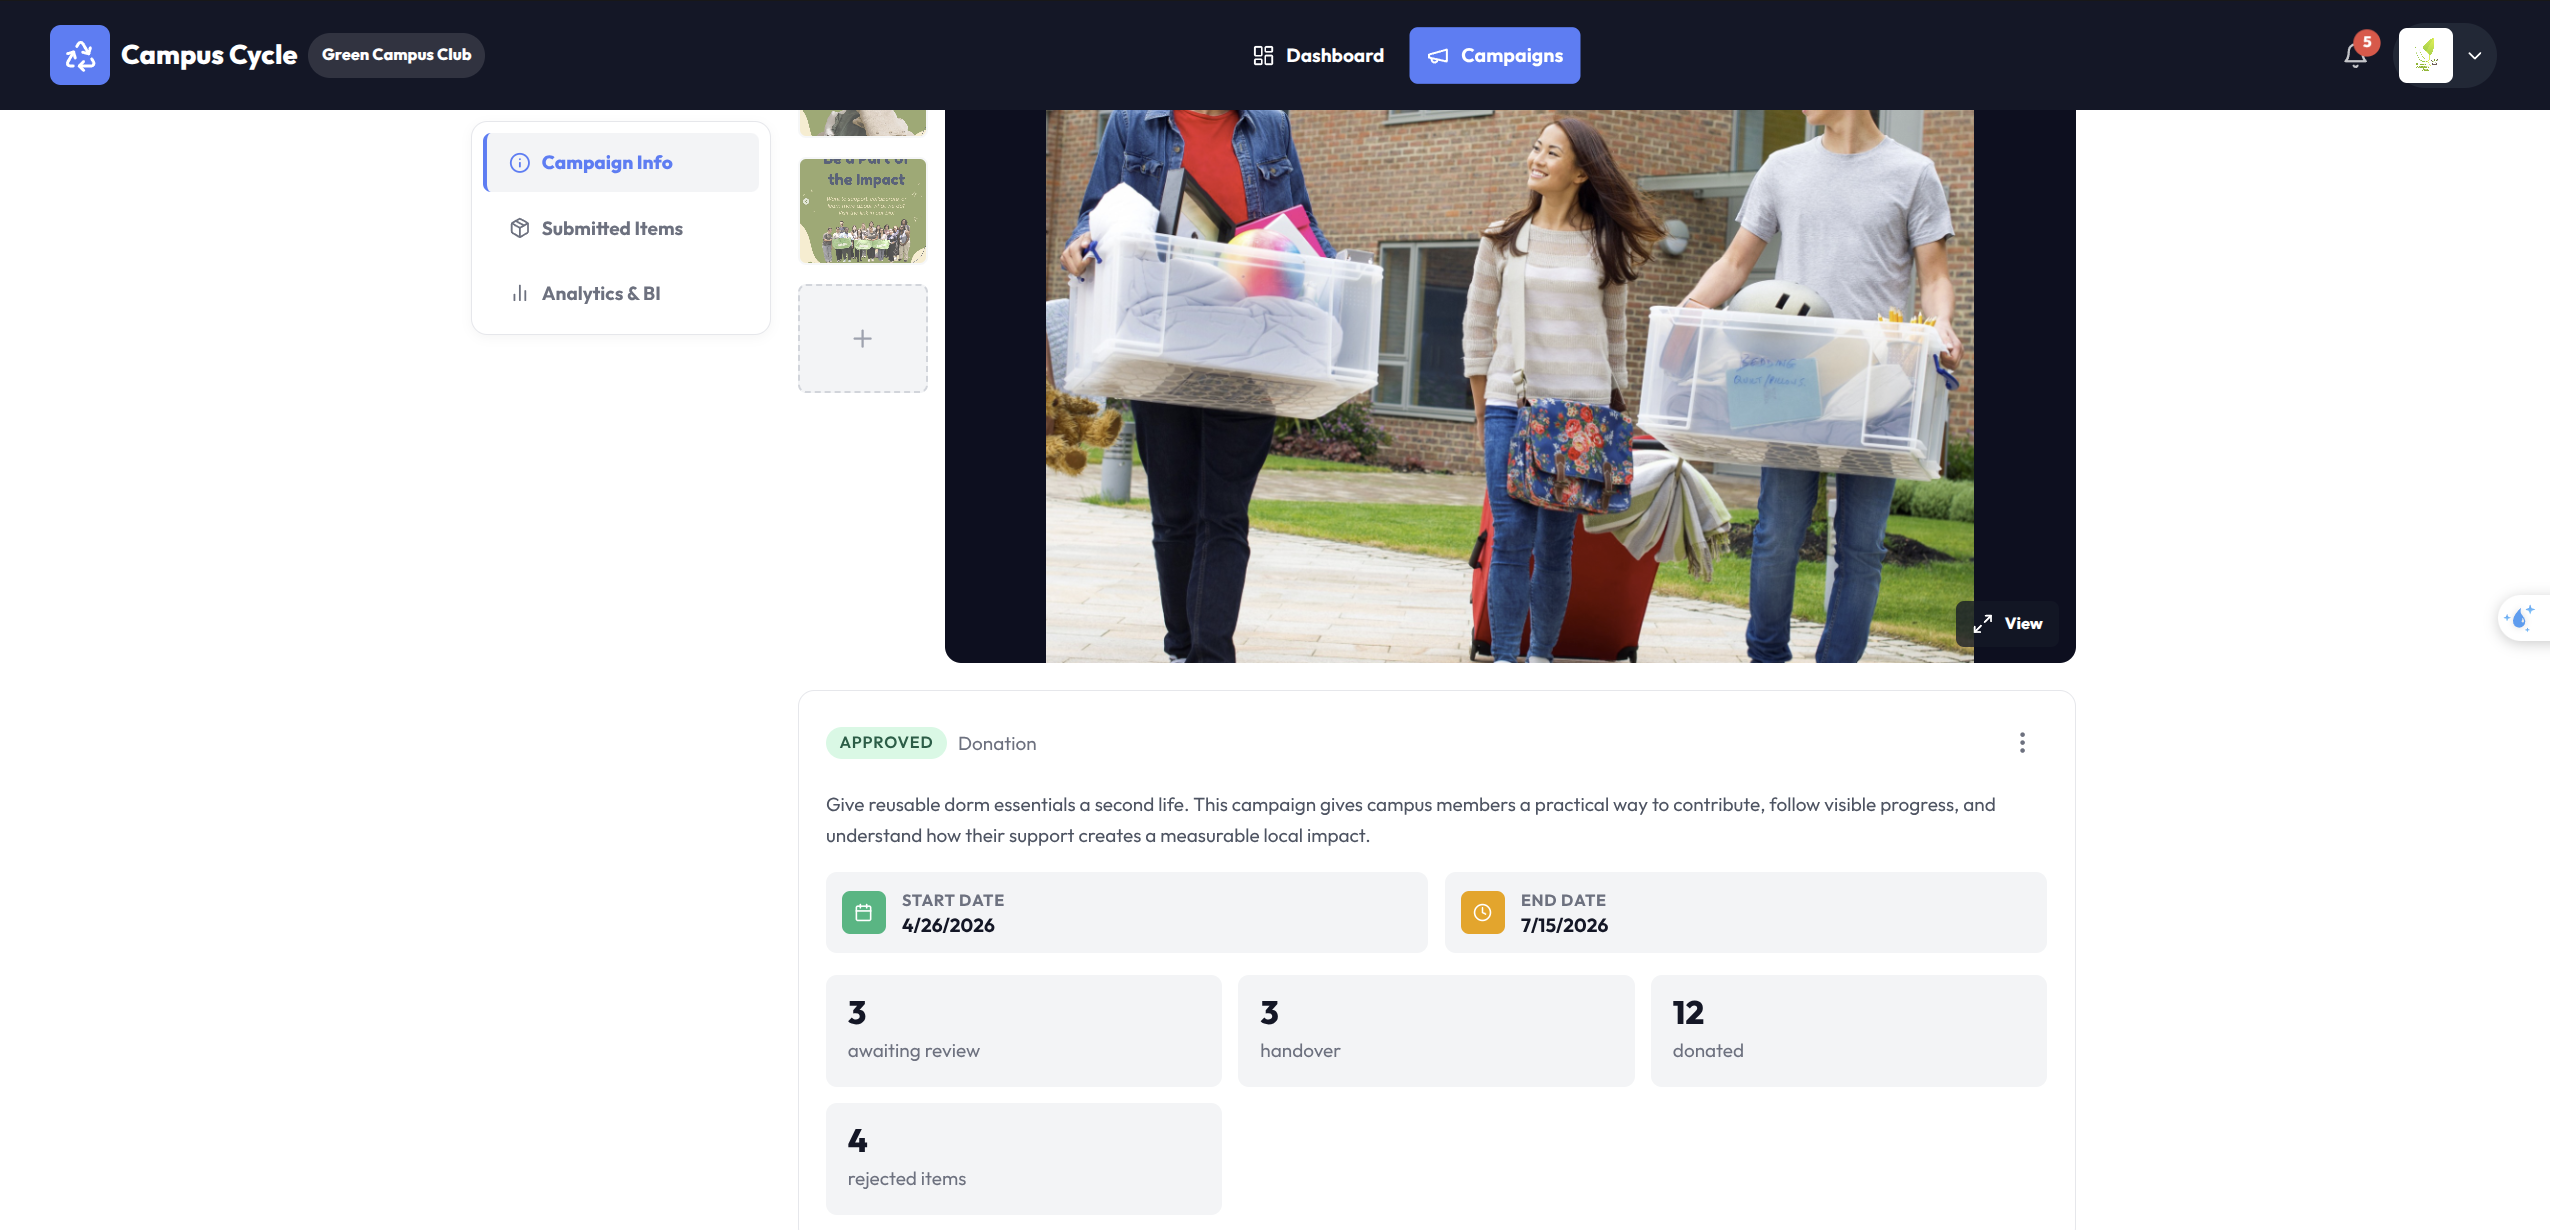
\includegraphics[width=0.75\textwidth]{Campaign Detail Page.png}
\caption{Campaign Detail Page}
\label{fig:campaign-detail-org-page}
\end{figure}

Donated Item List Page: Quản lí các item được gửi đến tổ chức để quyên góp.

\begin{figure}[H]
\centering
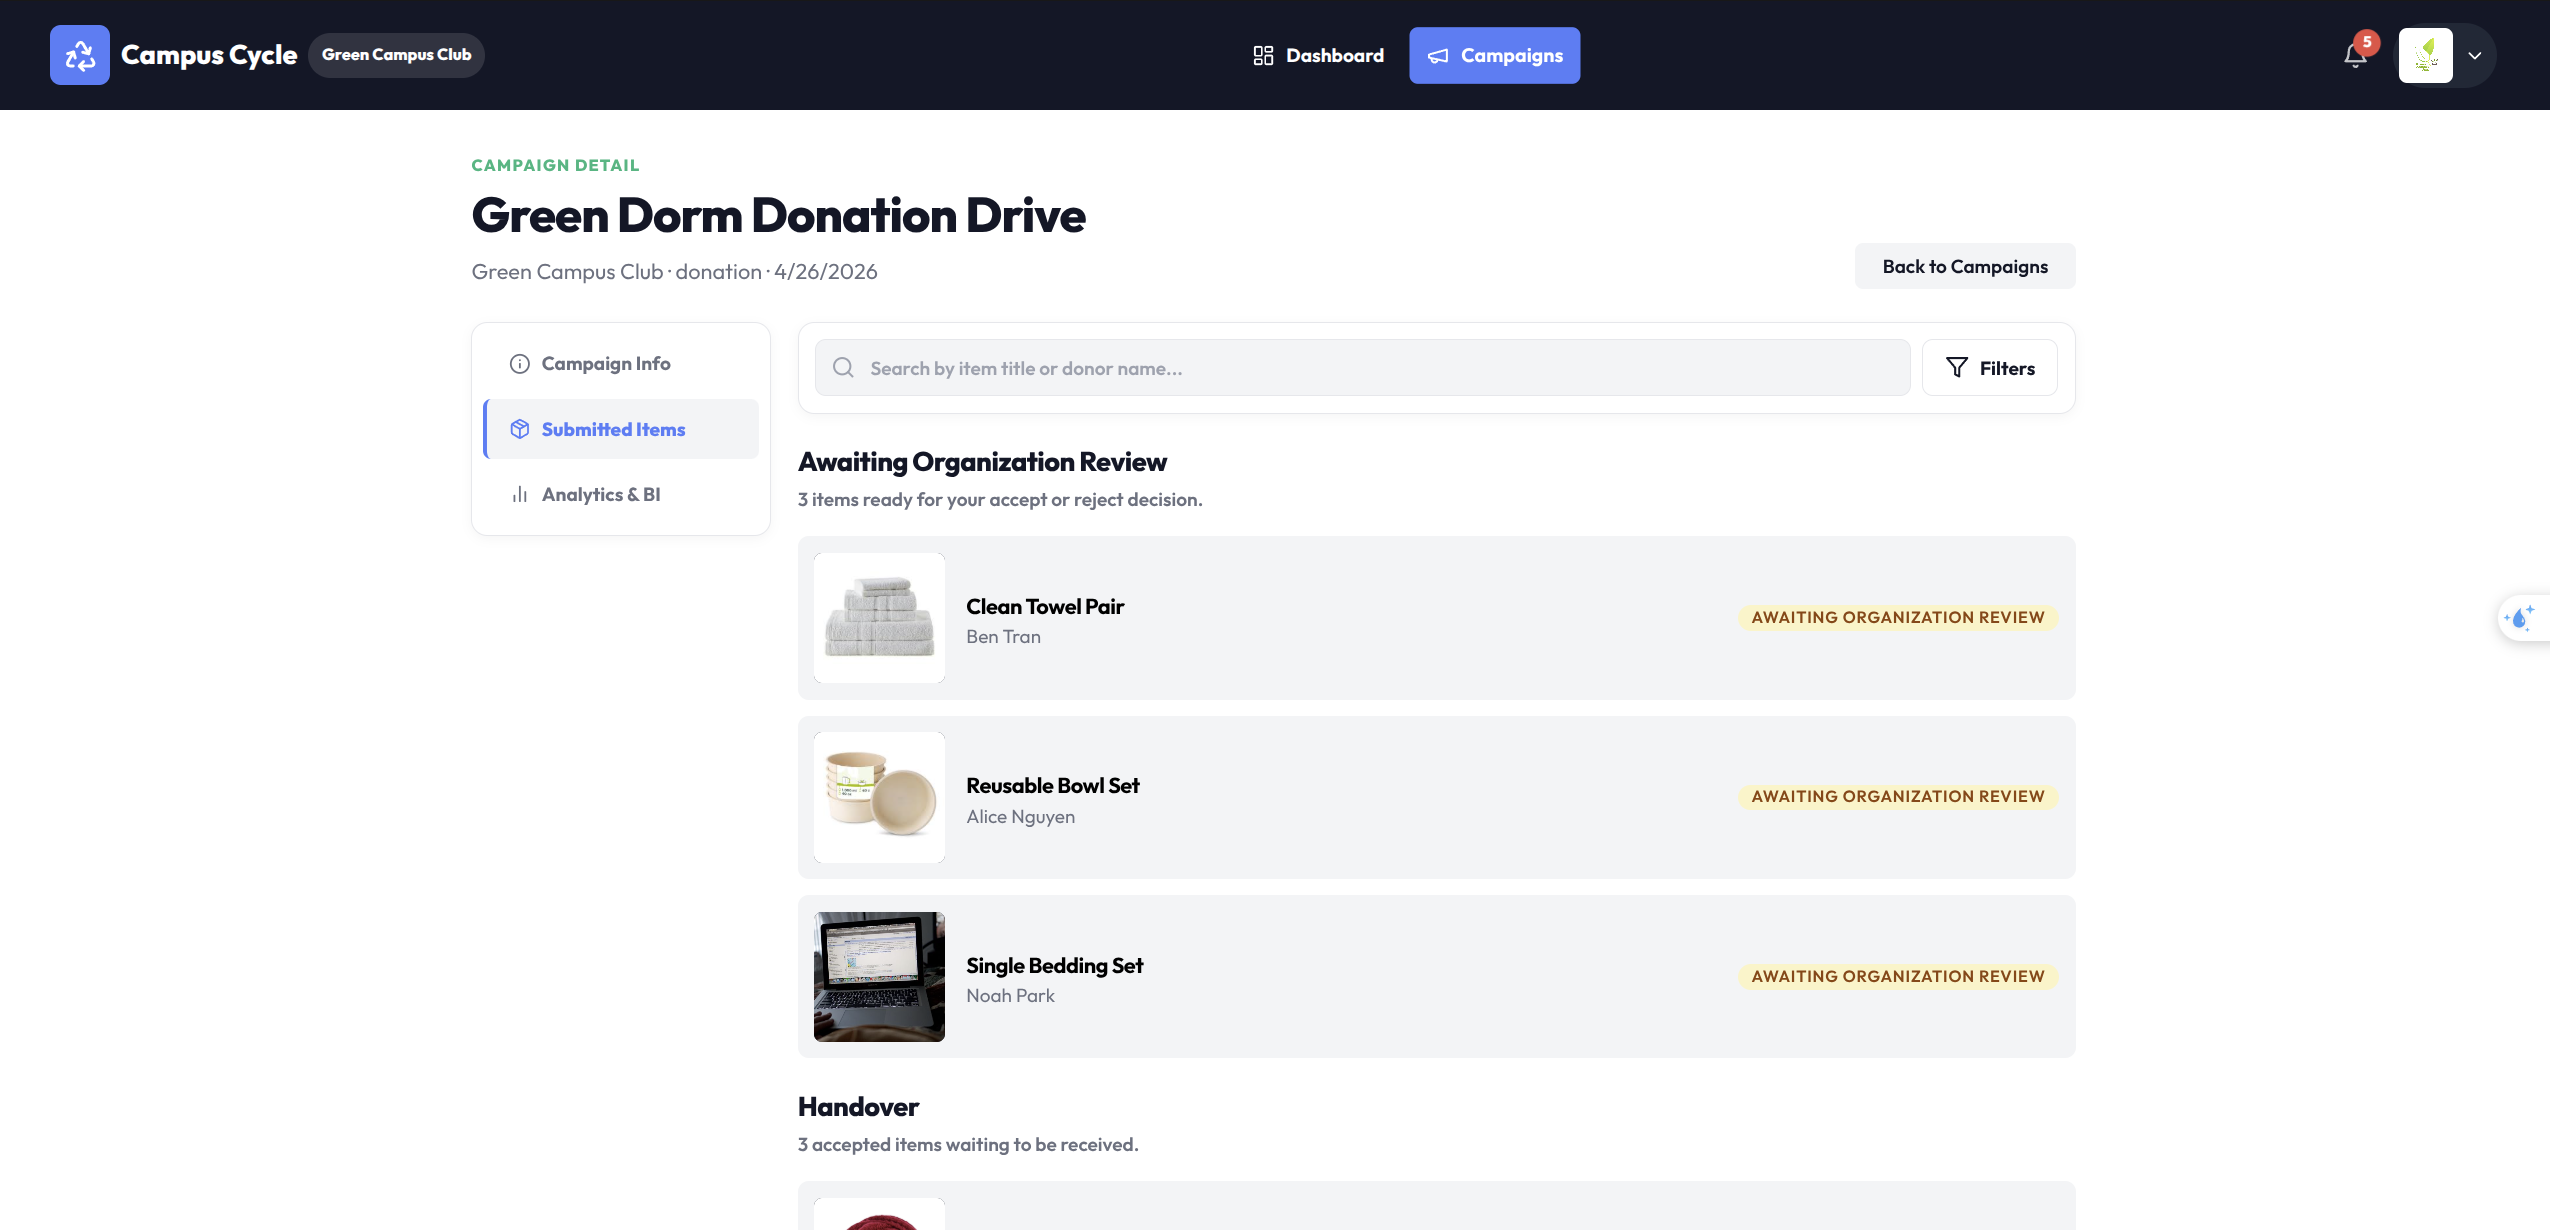
\includegraphics[width=0.75\textwidth]{Donated Item List Page.png}
\caption{Donated Item List Page}
\label{fig:donated-item-list-page}
\end{figure}

Approval Page: Cho phép xem thông tin chi tiết của item được gửi đến tổ chức, để approve hoặc reject.

\begin{figure}[H]
\centering
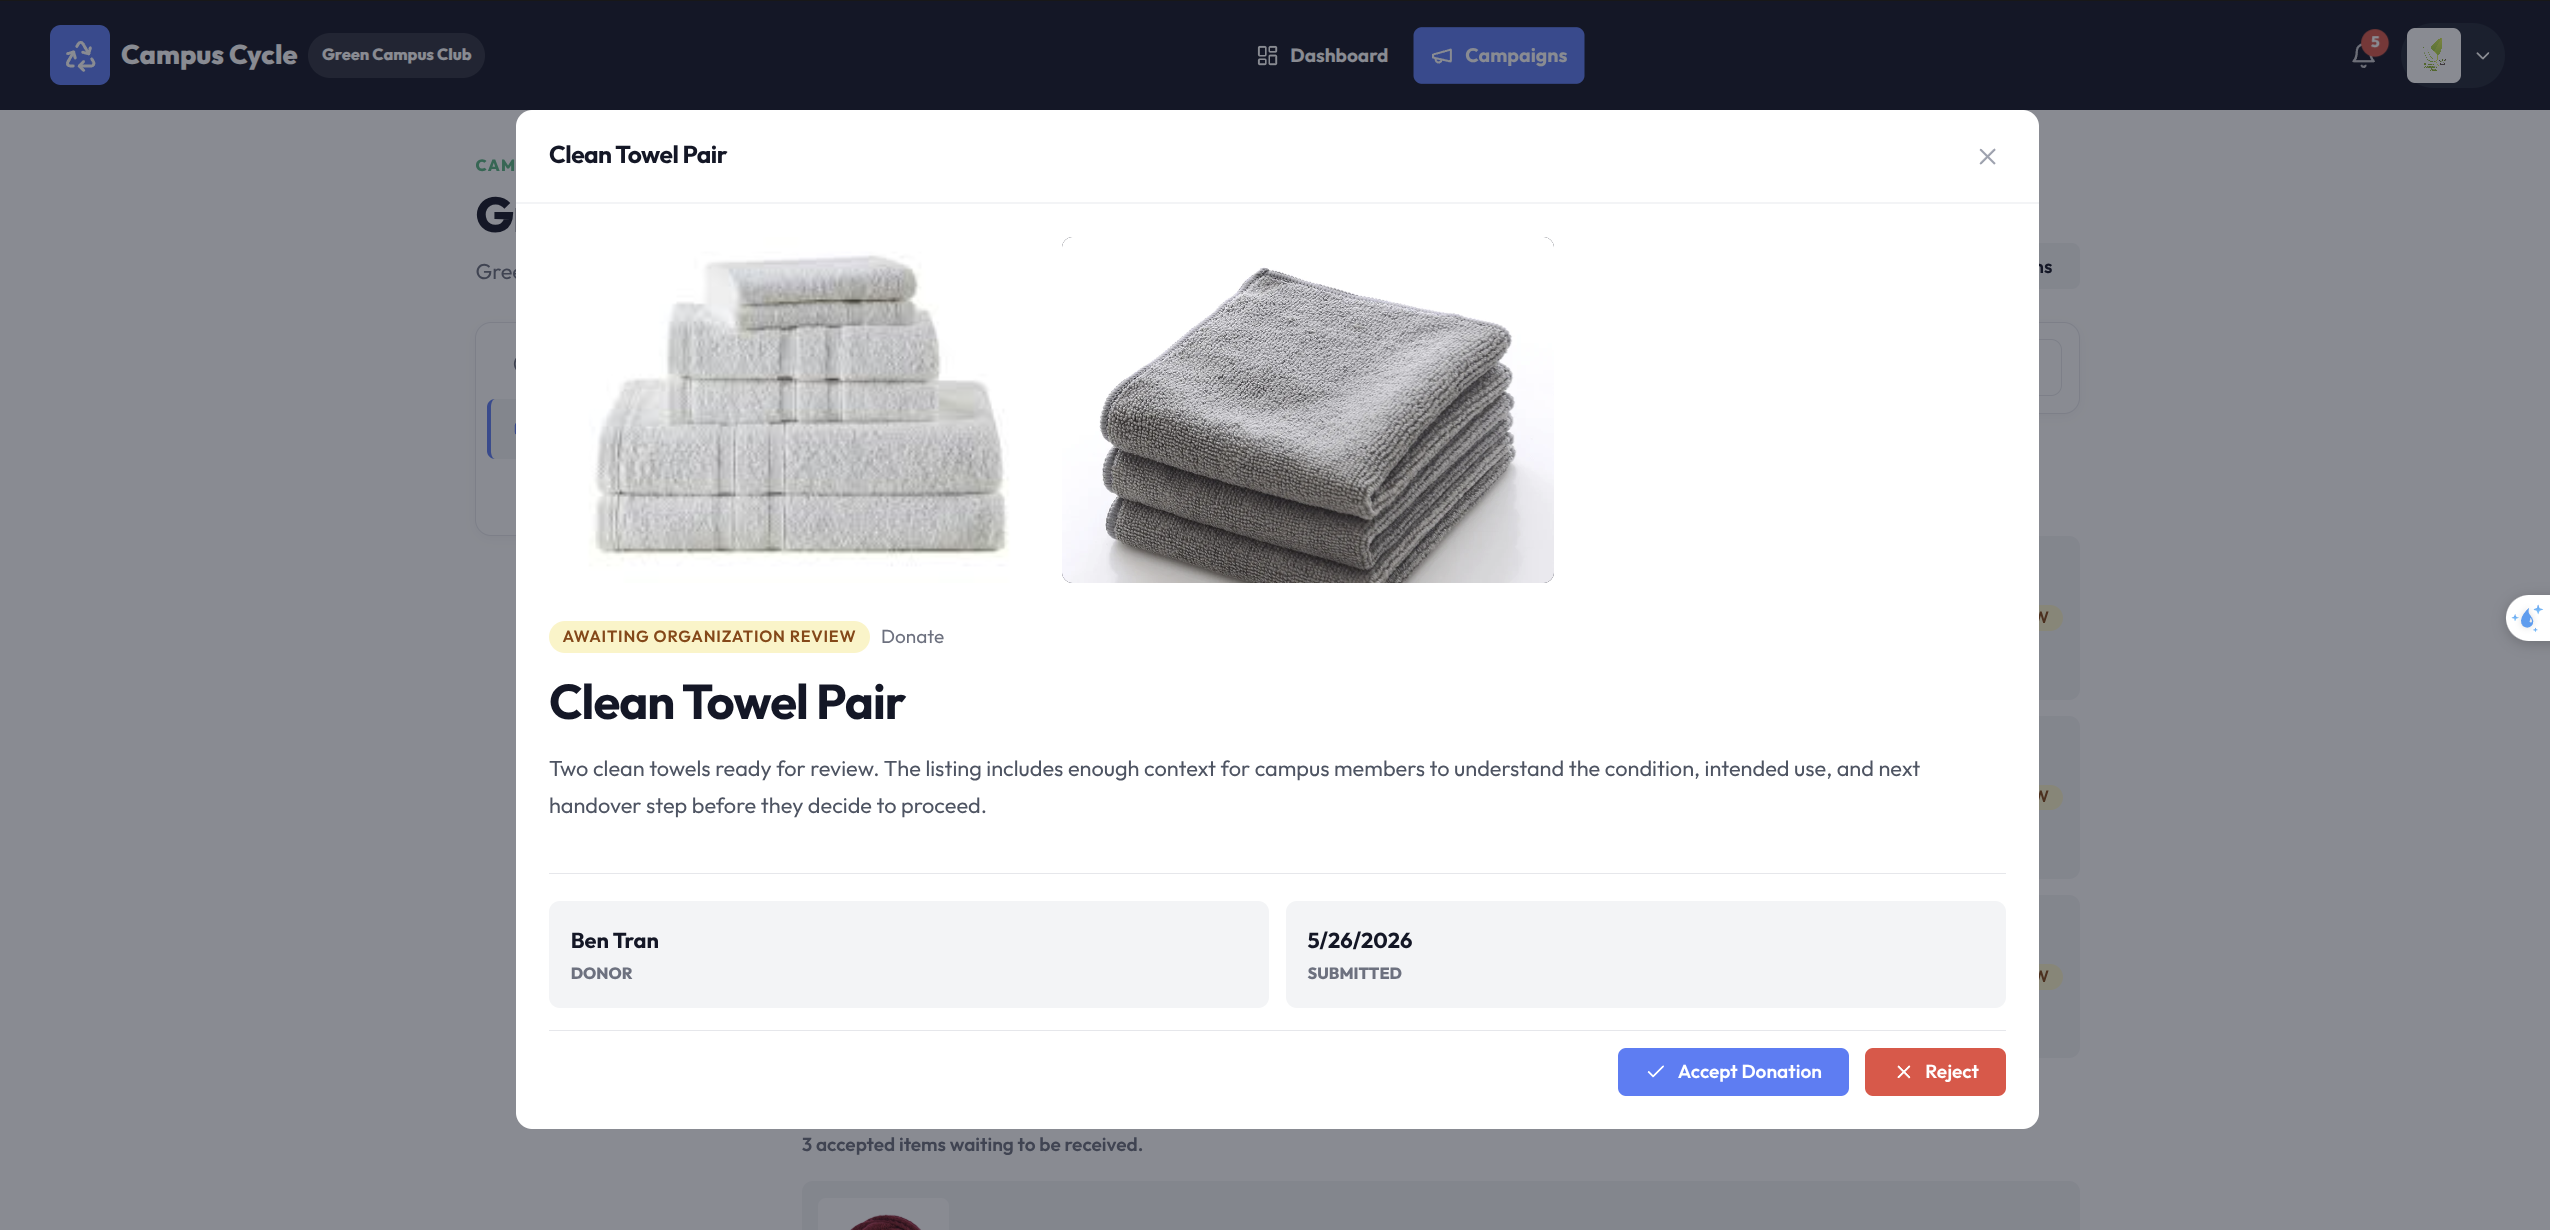
\includegraphics[width=0.75\textwidth]{Donation Item Approval Detail Page.png}
\caption{Donated Item Detail Page}
\label{fig:donated-item-detail-page}
\end{figure}

Handover Page: Cho phép cập nhật trạng thái bàn giao vật phẩm sau khi đã approve, ví dụ như đang chờ bàn giao, đã nhận hoặc từ chối bàn giao.

\begin{figure}[H]
\centering
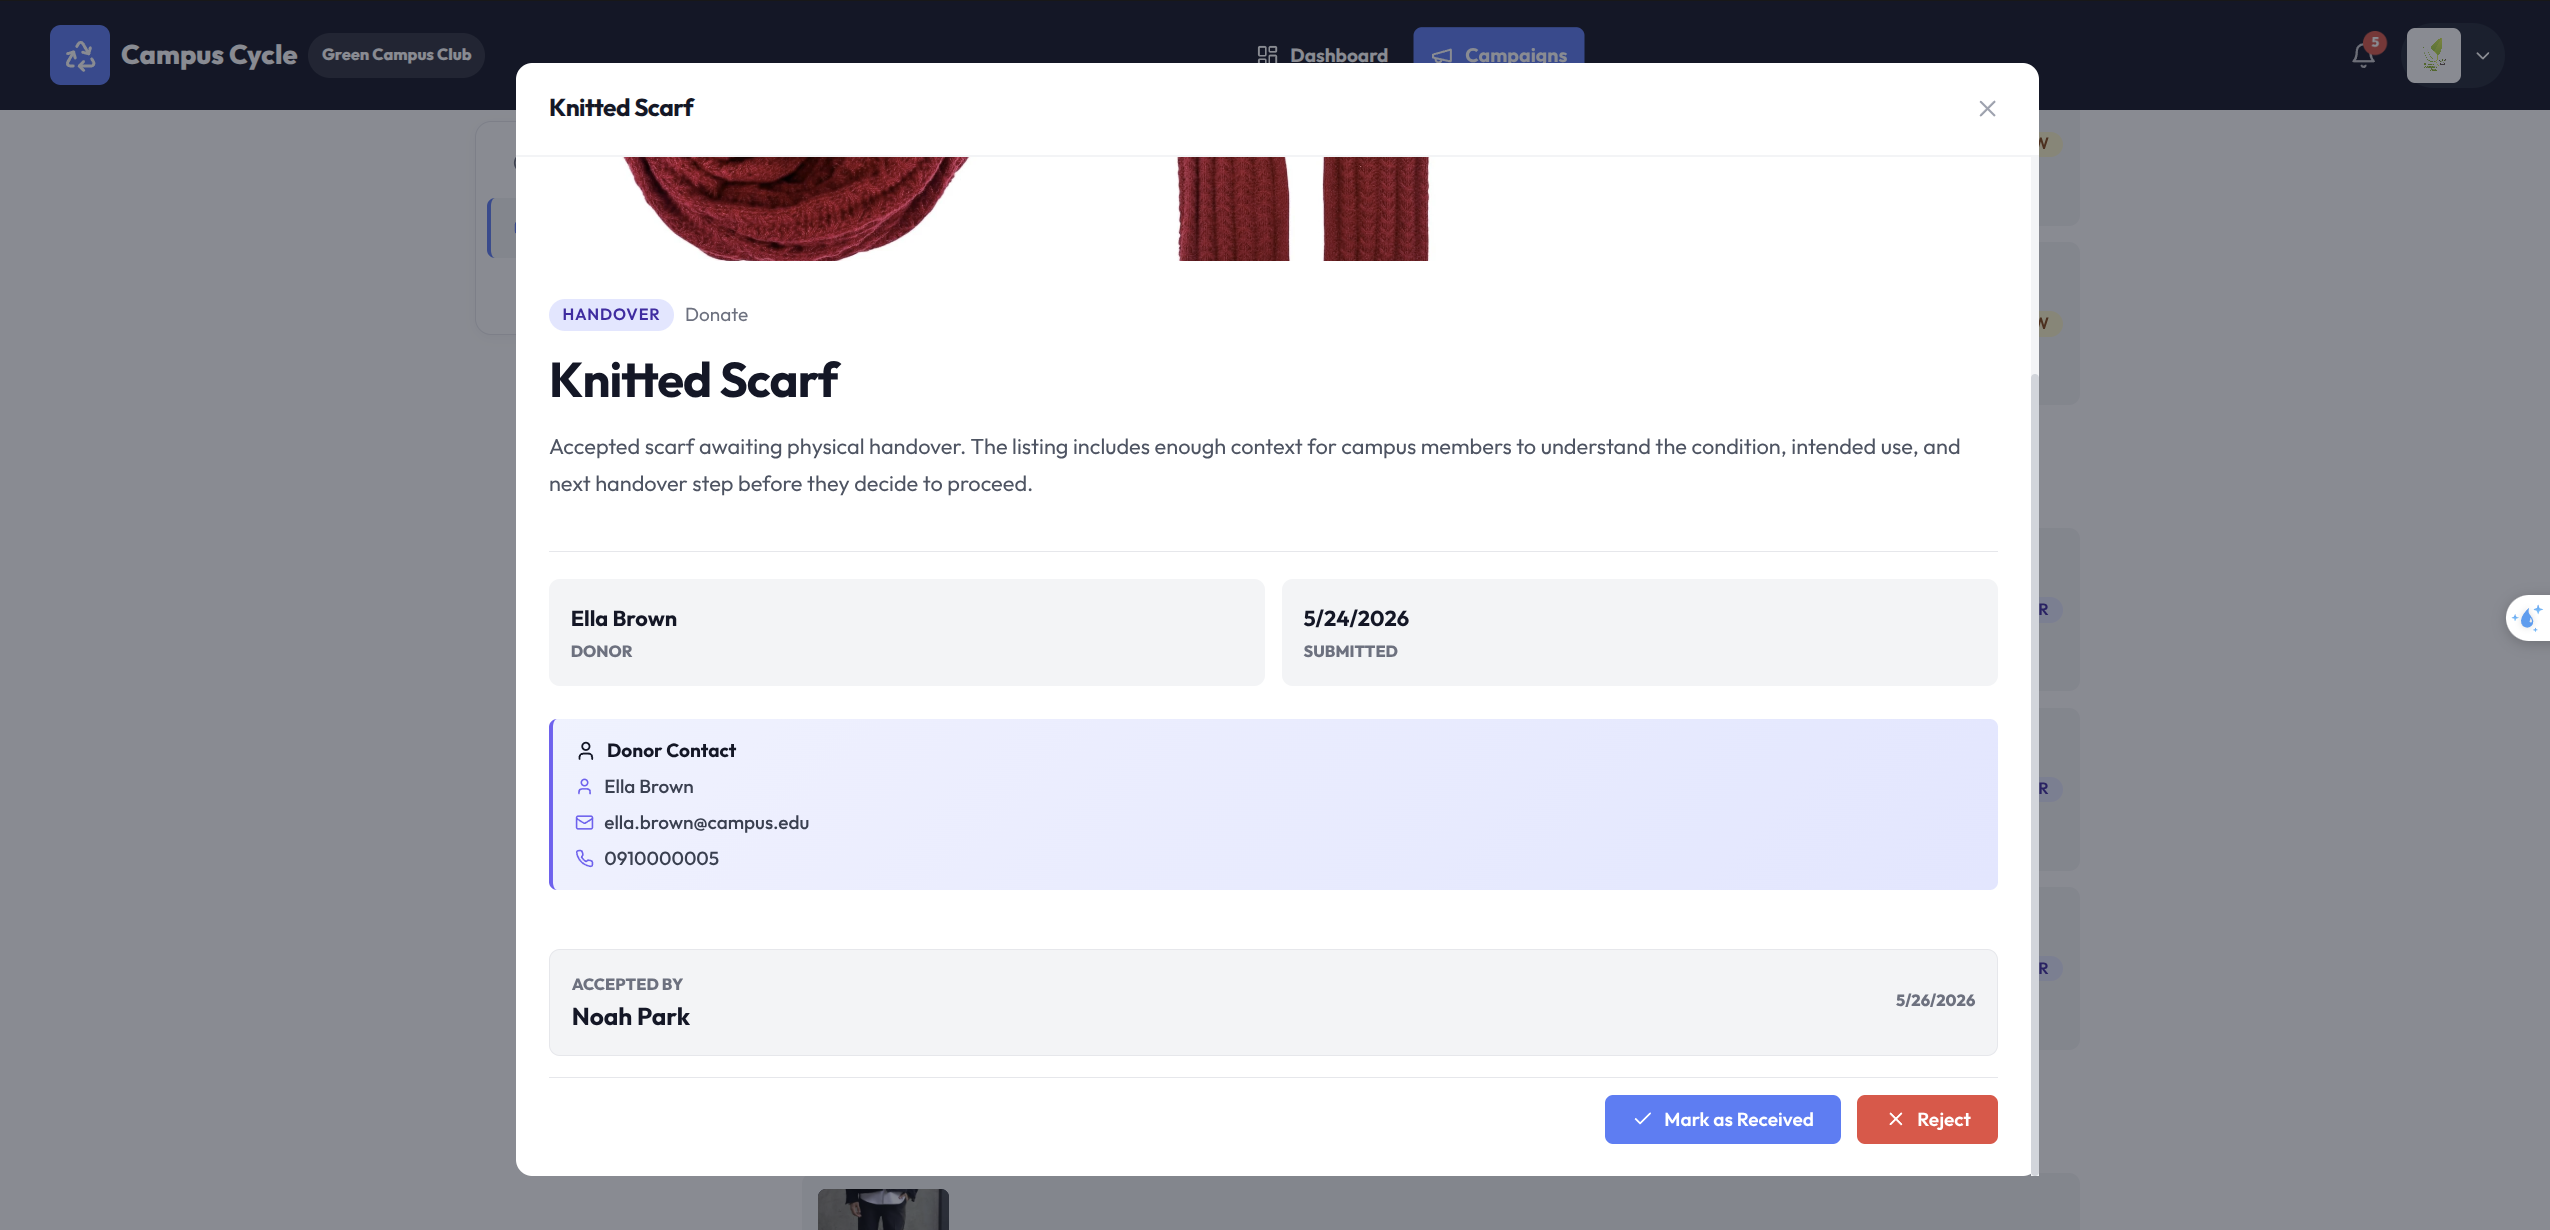
\includegraphics[width=0.75\textwidth]{Donation Item Approval Form.png}
\caption{Handover Page}
\label{fig:approval-page}
\end{figure}

Campaign Statistics Page: Hiển thị số tiền, số lượng vật phẩm và progress của campaign.

\begin{figure}[H]
\centering
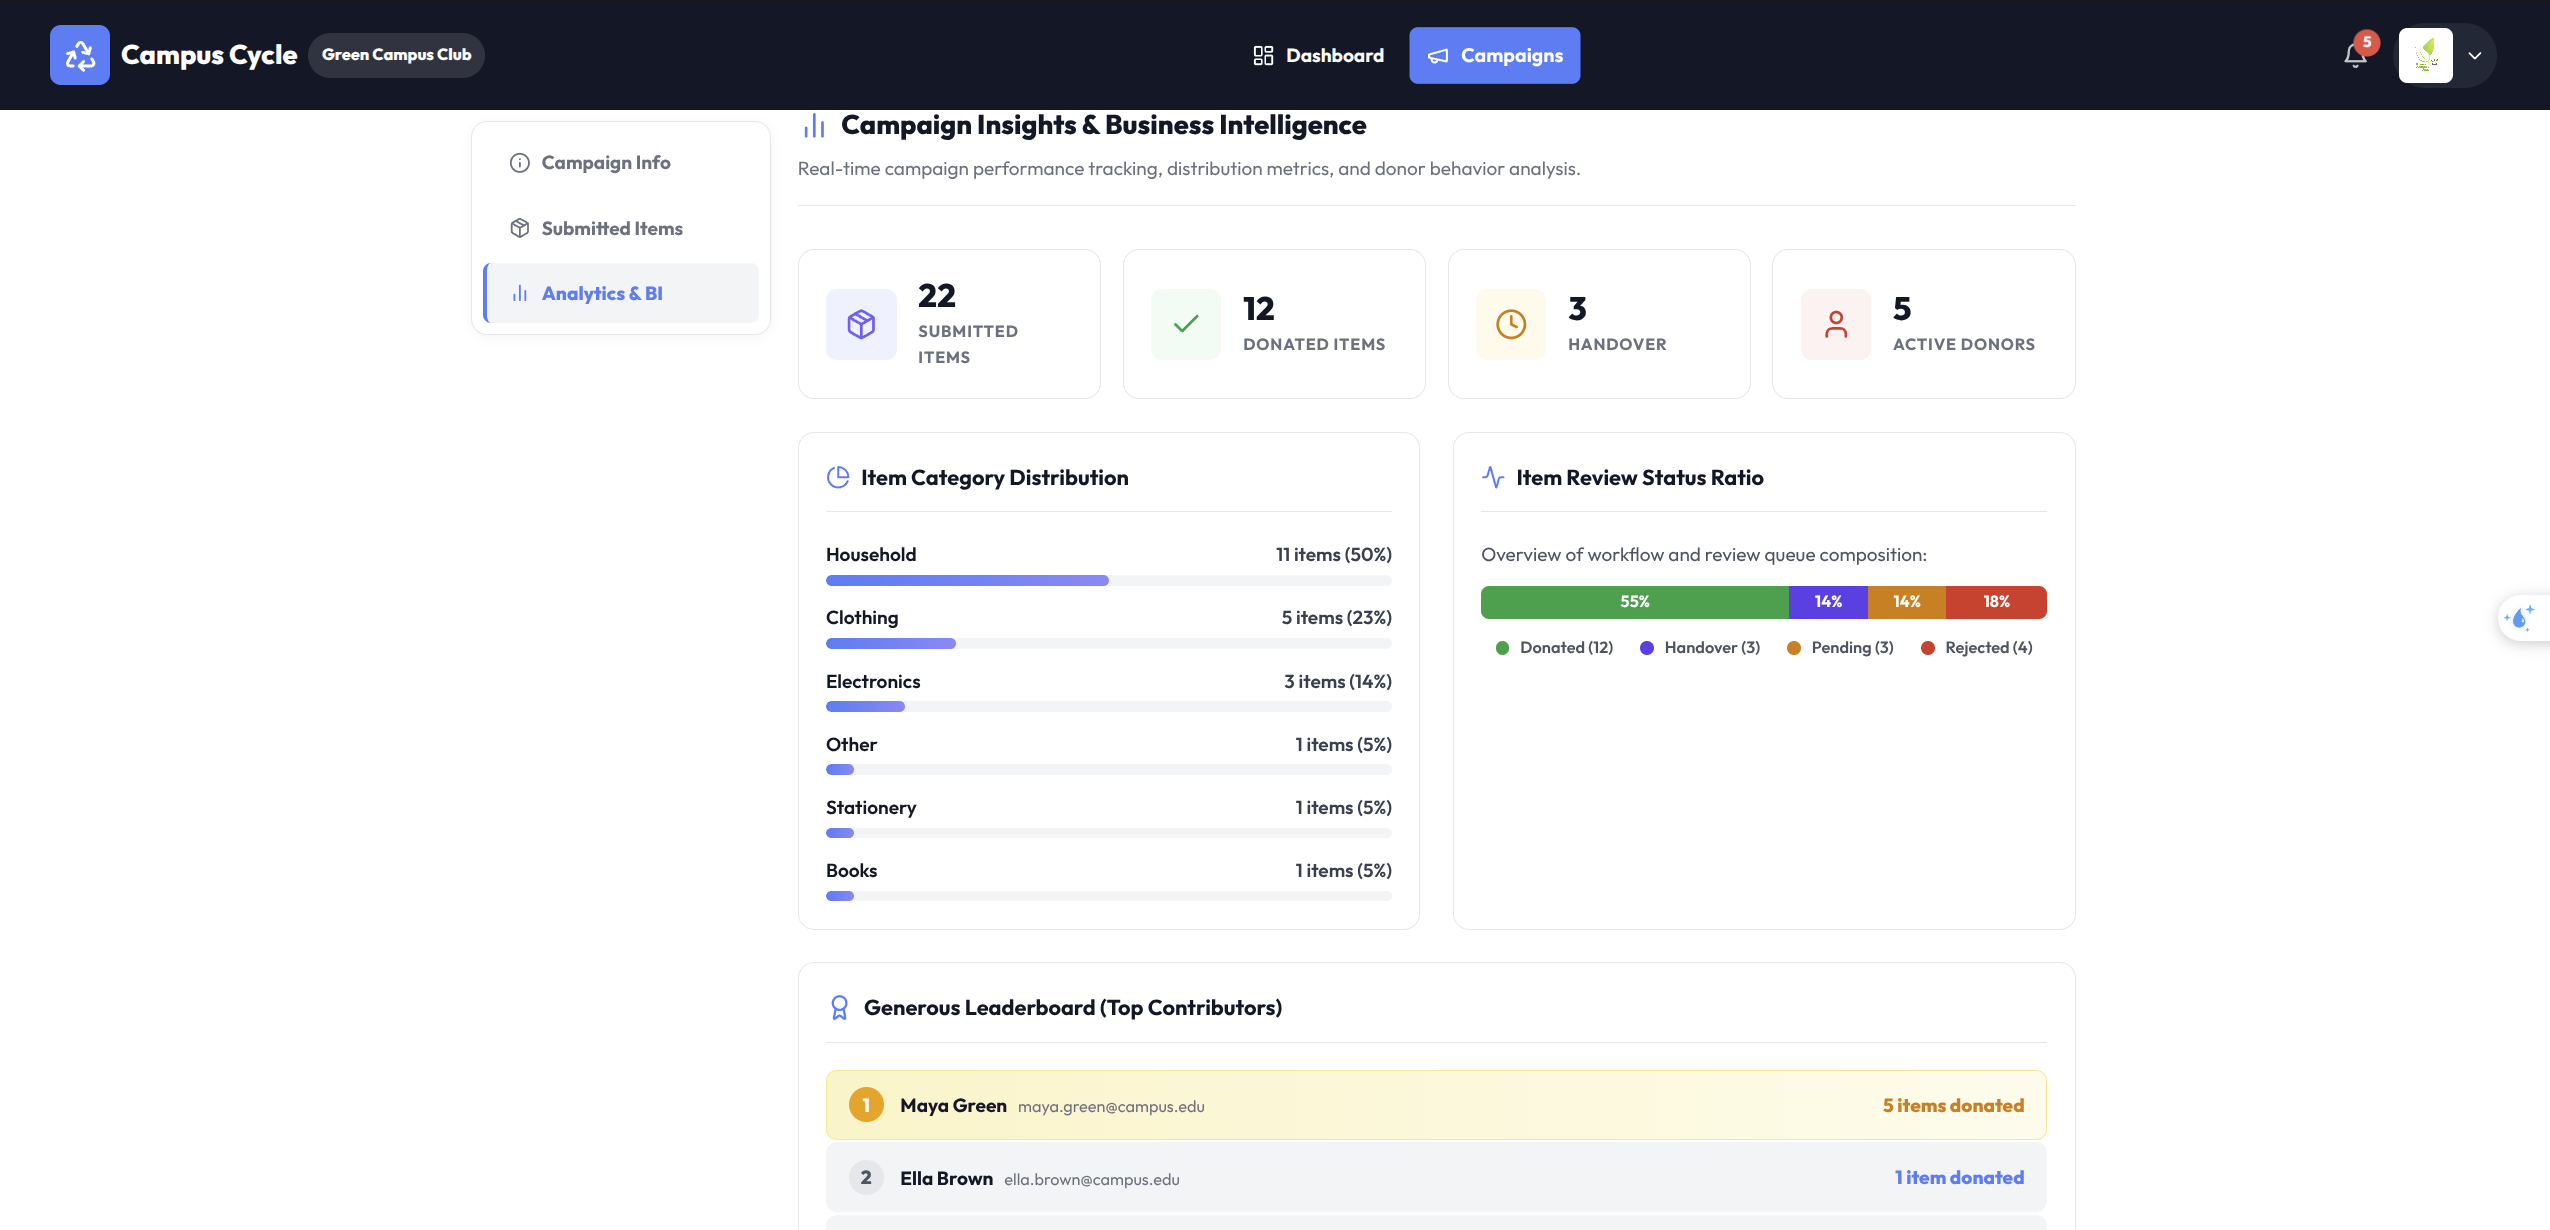
\includegraphics[width=0.75\textwidth]{Campaign Statistics Page.png}
\caption{Campaign Statistics Page}
\label{fig:campaign-statistics-page}
\end{figure}

\subsection{Nhóm giao diện quản trị hệ thống}

Nhóm giao diện này dành cho System Admin, là người có quyền quản lý toàn bộ hệ thống. System Admin có thể theo dõi toàn bộ hoạt động của hệ thống, quản lý user accounts, organizations, categories, items, transactions và campaigns.

Admin Dashboard: Hiển thị overview về số lượng user, item, campaign và transaction trong hệ thống.

\begin{figure}[H]
\centering
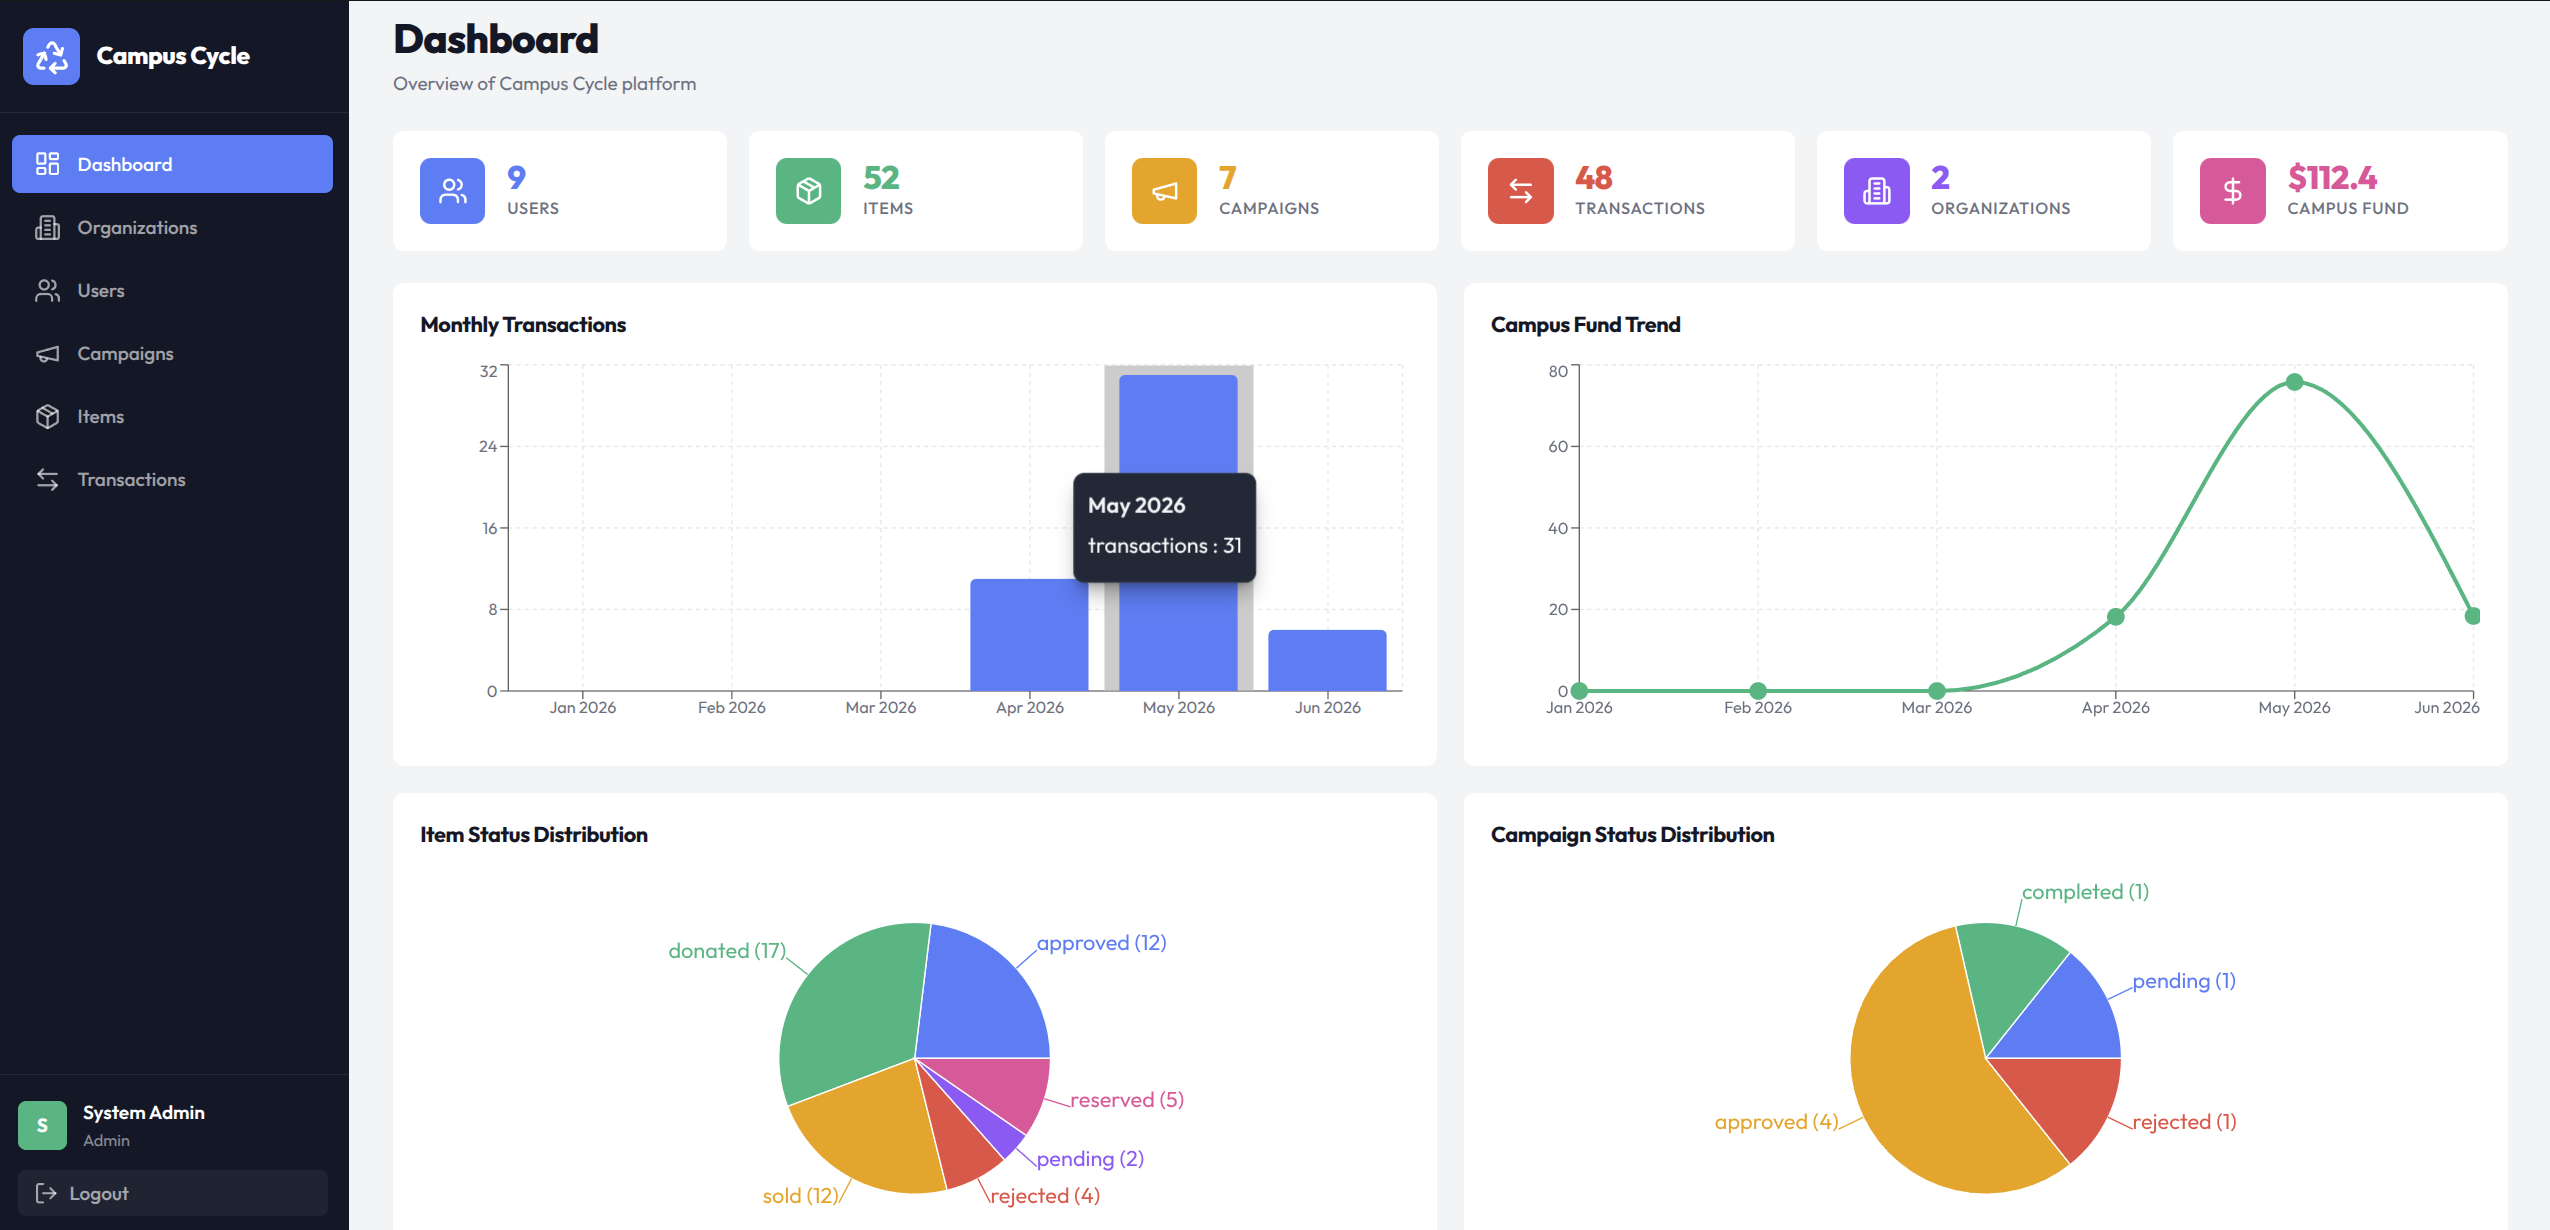
\includegraphics[width=0.75\textwidth]{Admin Dashboard.png}
\caption{Admin Dashboard}
\label{fig:admin-dashboard}
\end{figure}

User Management Page: Cho phép xem, tìm kiếm và quản lý user accounts.

\begin{figure}[H]
\centering
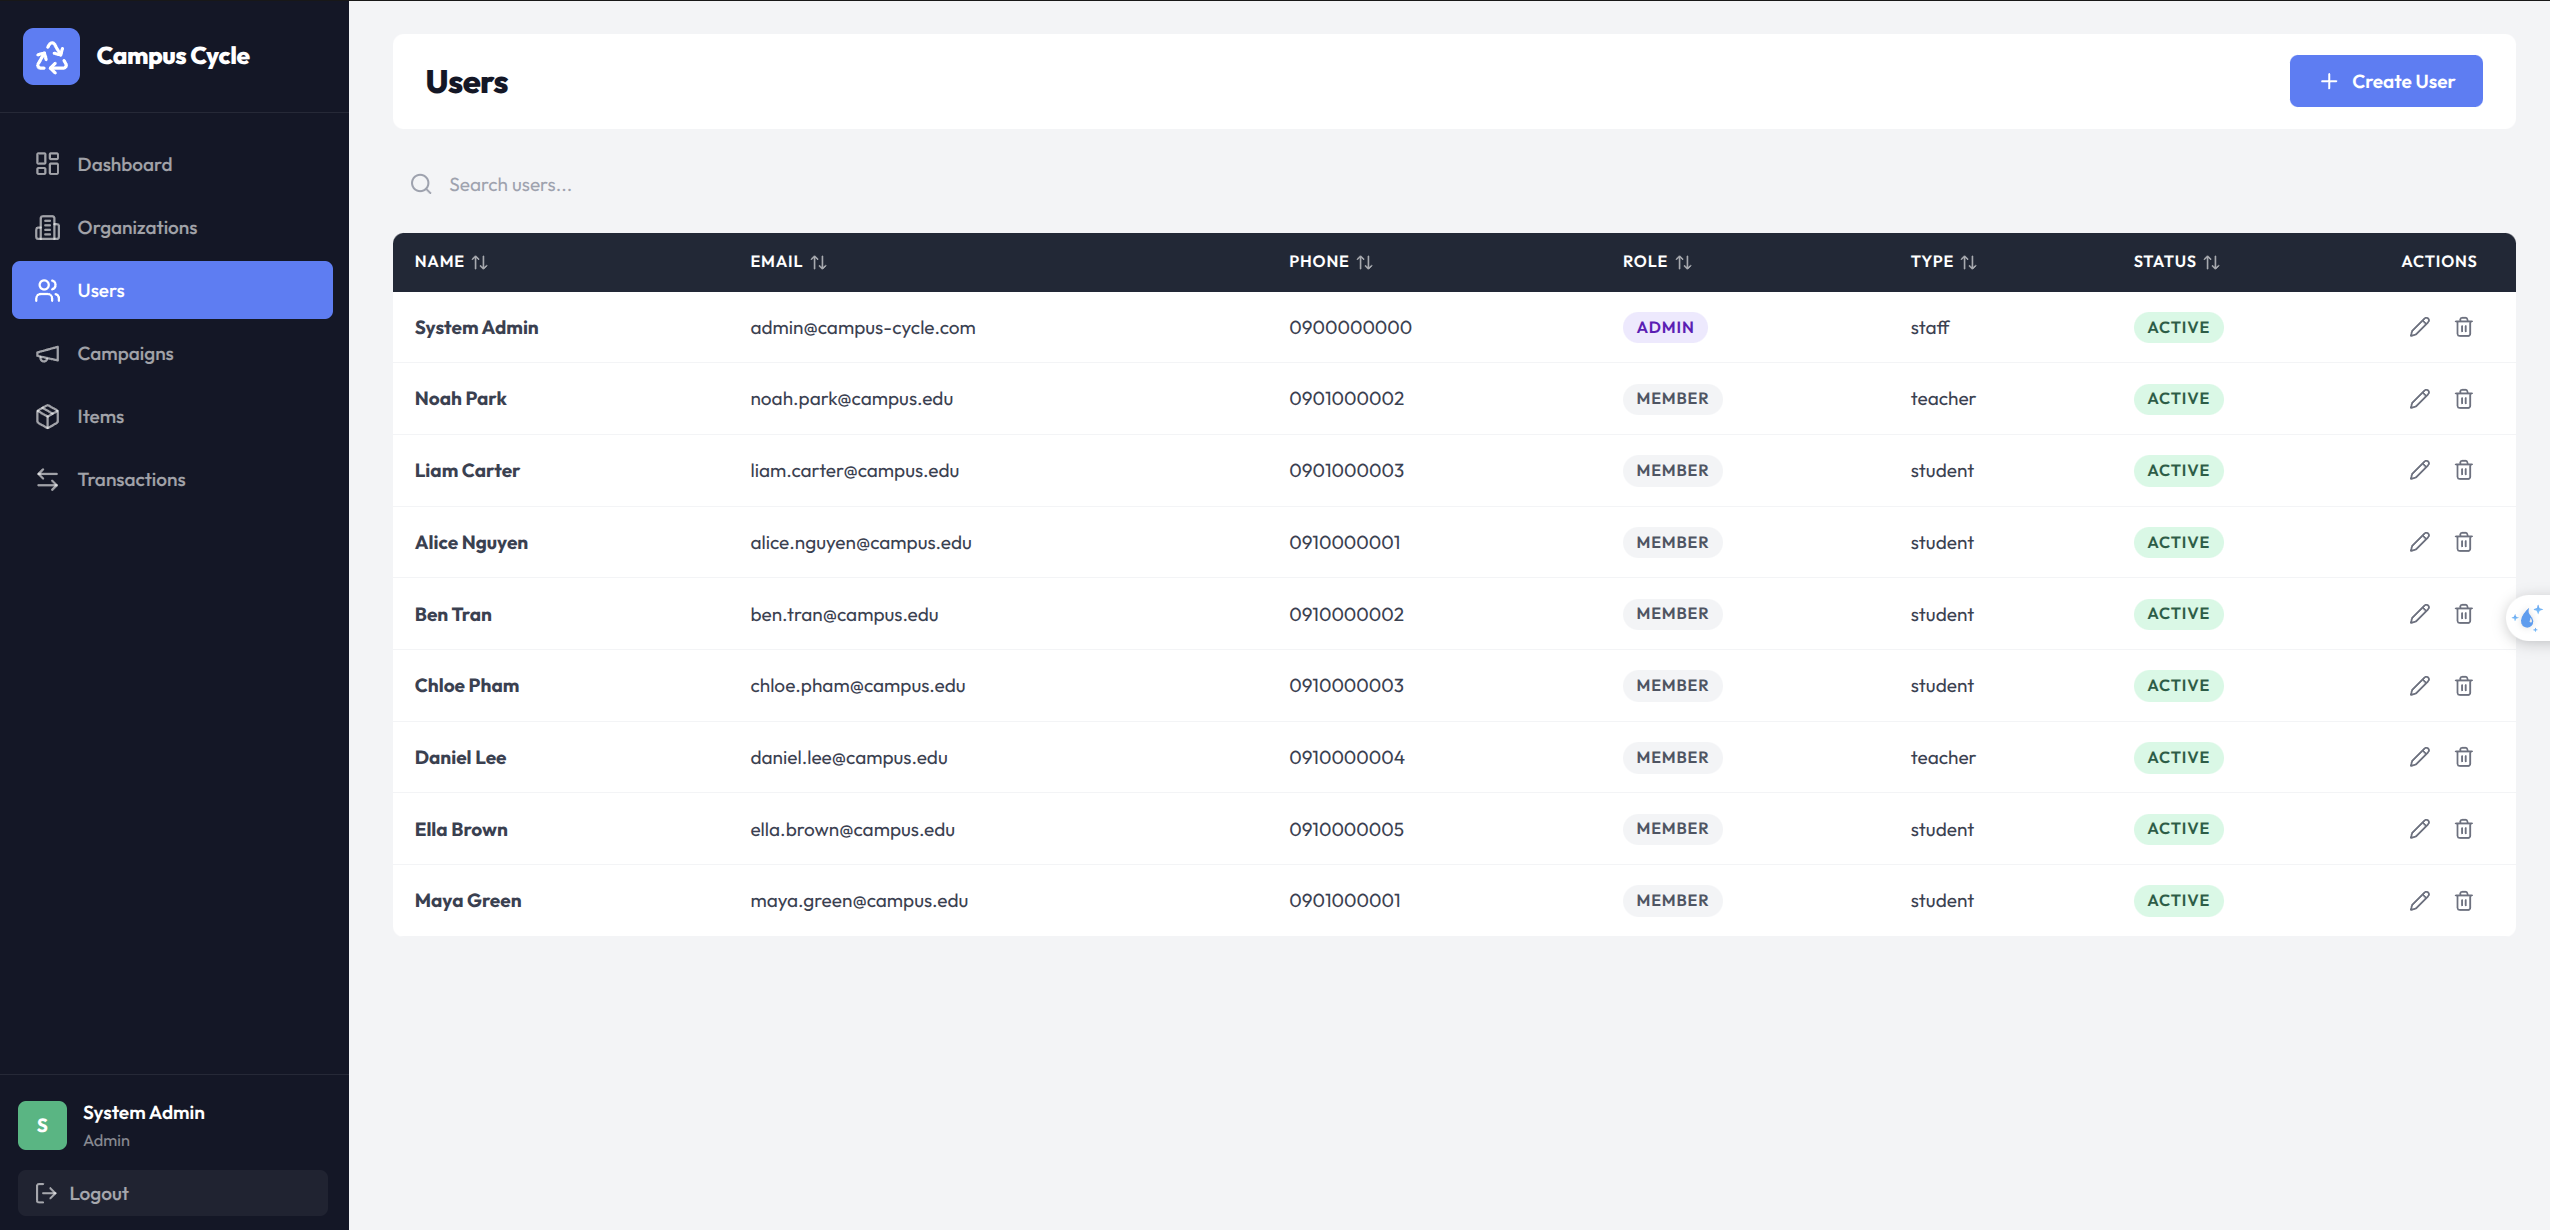
\includegraphics[width=0.75\textwidth]{User Management Page.png}
\caption{User Management Page}
\label{fig:user-management-page}
\end{figure}

Organization Management Page: Cho phép xem và quản lý các organizations tham gia hệ thống.

\begin{figure}[H]
\centering
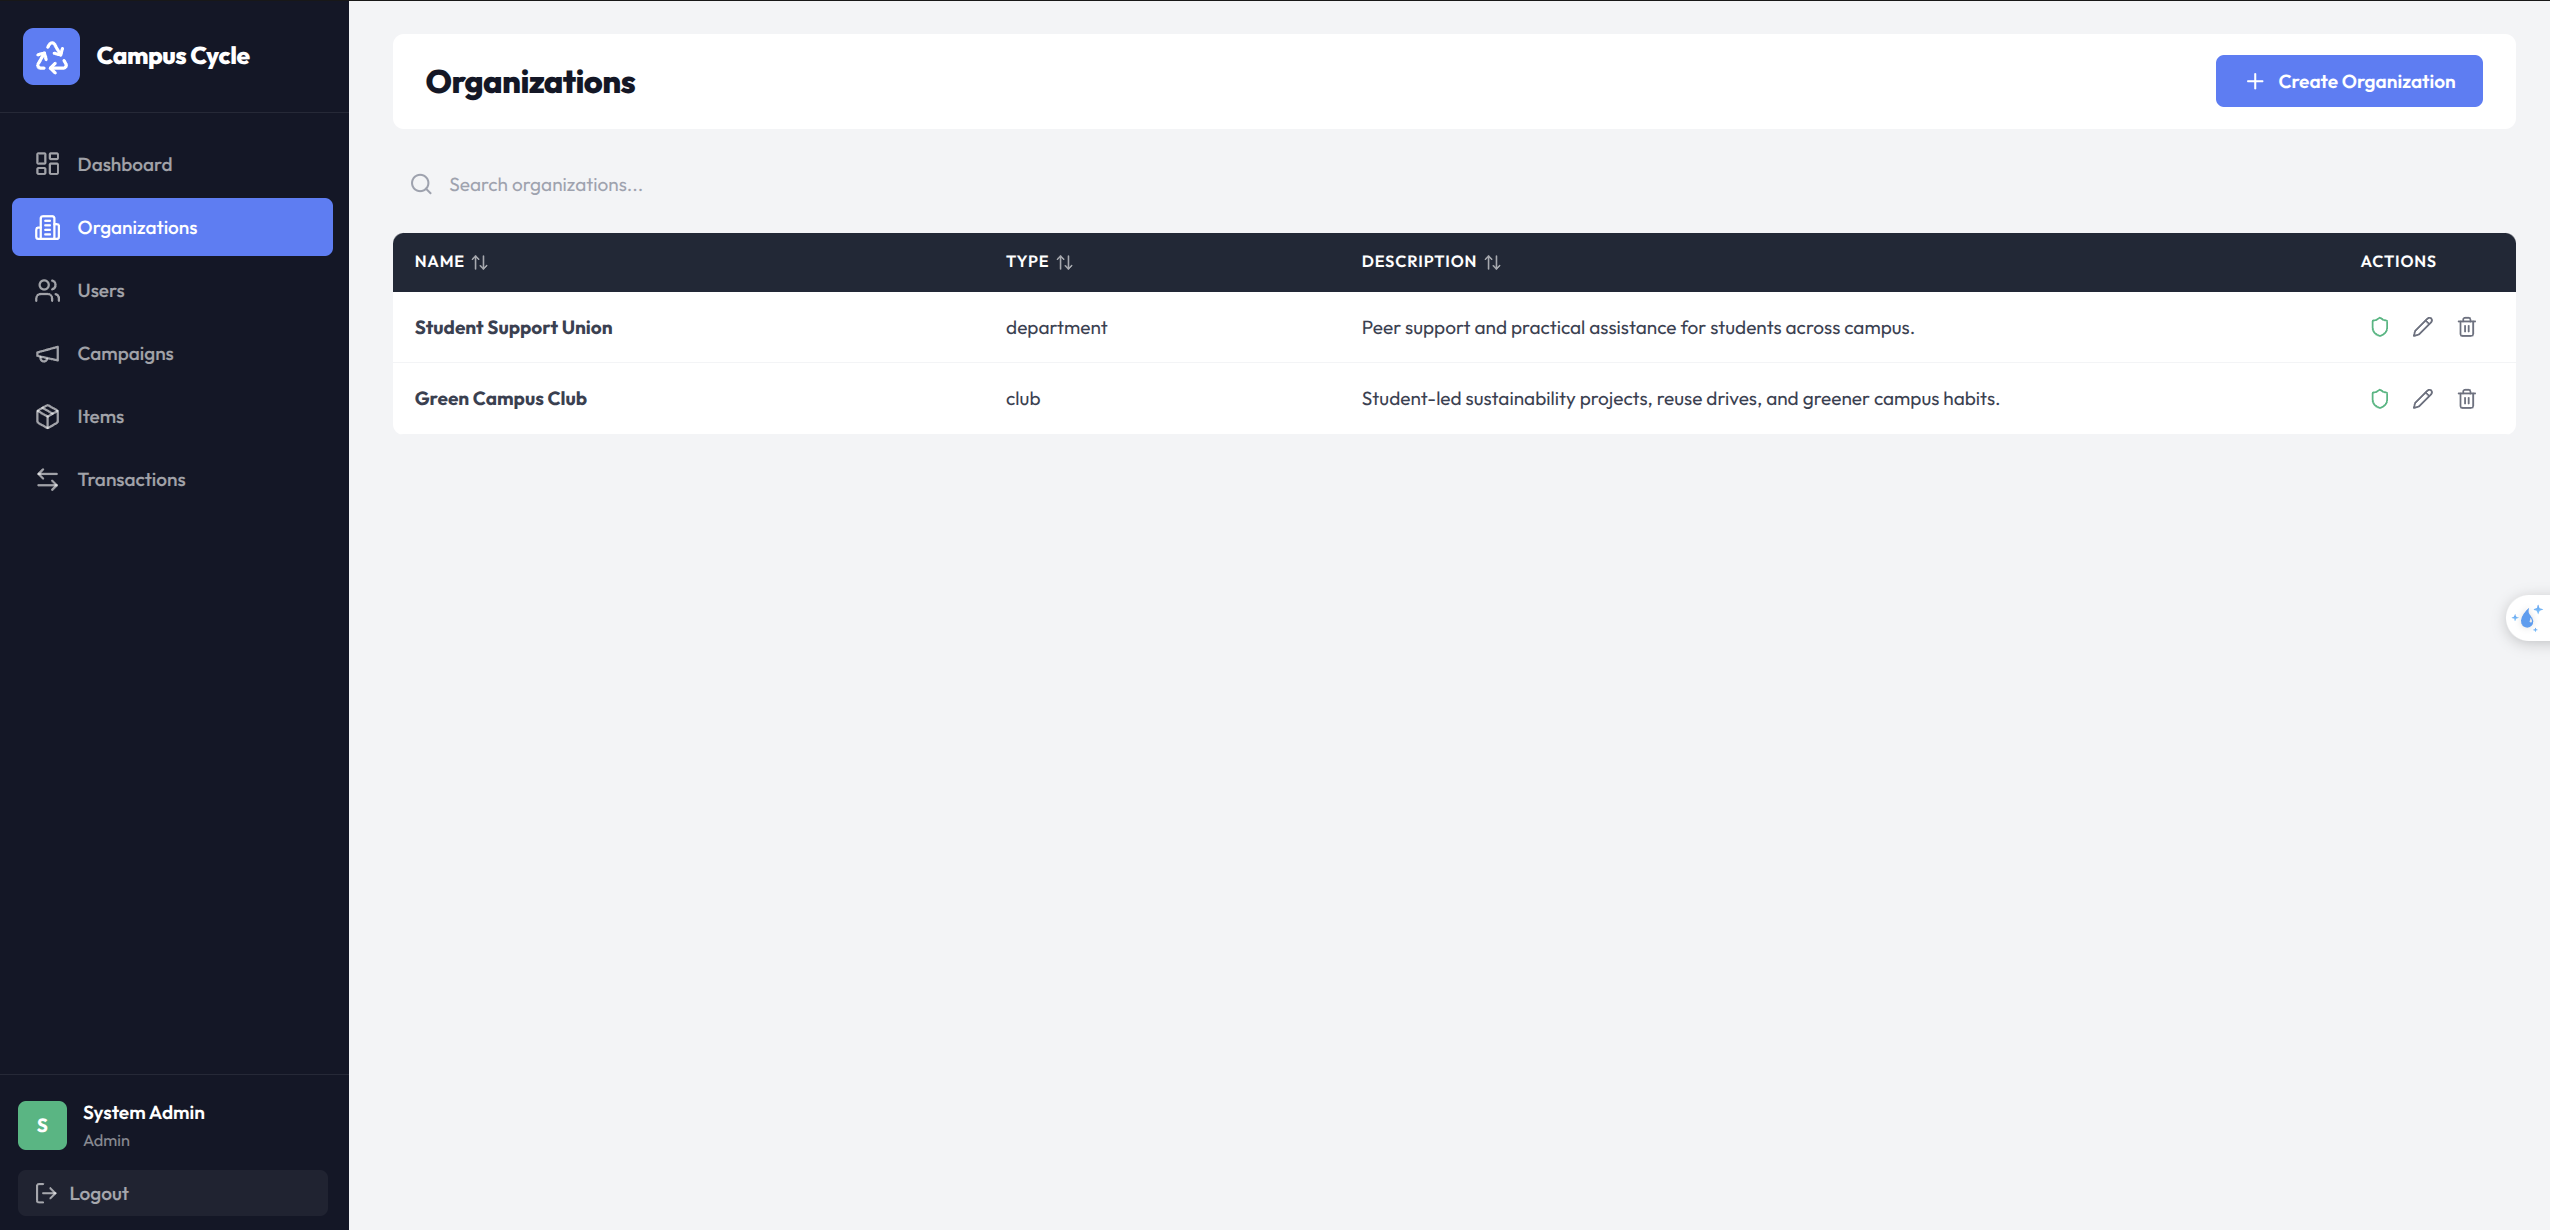
\includegraphics[width=0.75\textwidth]{Organization Management Page.png}
\caption{Organization Management Page}
\label{fig:organization-management-page}
\end{figure}

Organization Admin Management Page: Cho phép system admin quản lý danh sách admin của một organization. Giao diện hiển thị các admin hiện tại của organization và hỗ trợ thêm hoặc xóa admin khỏi organization đó.

\begin{figure}[H]
    \centering
    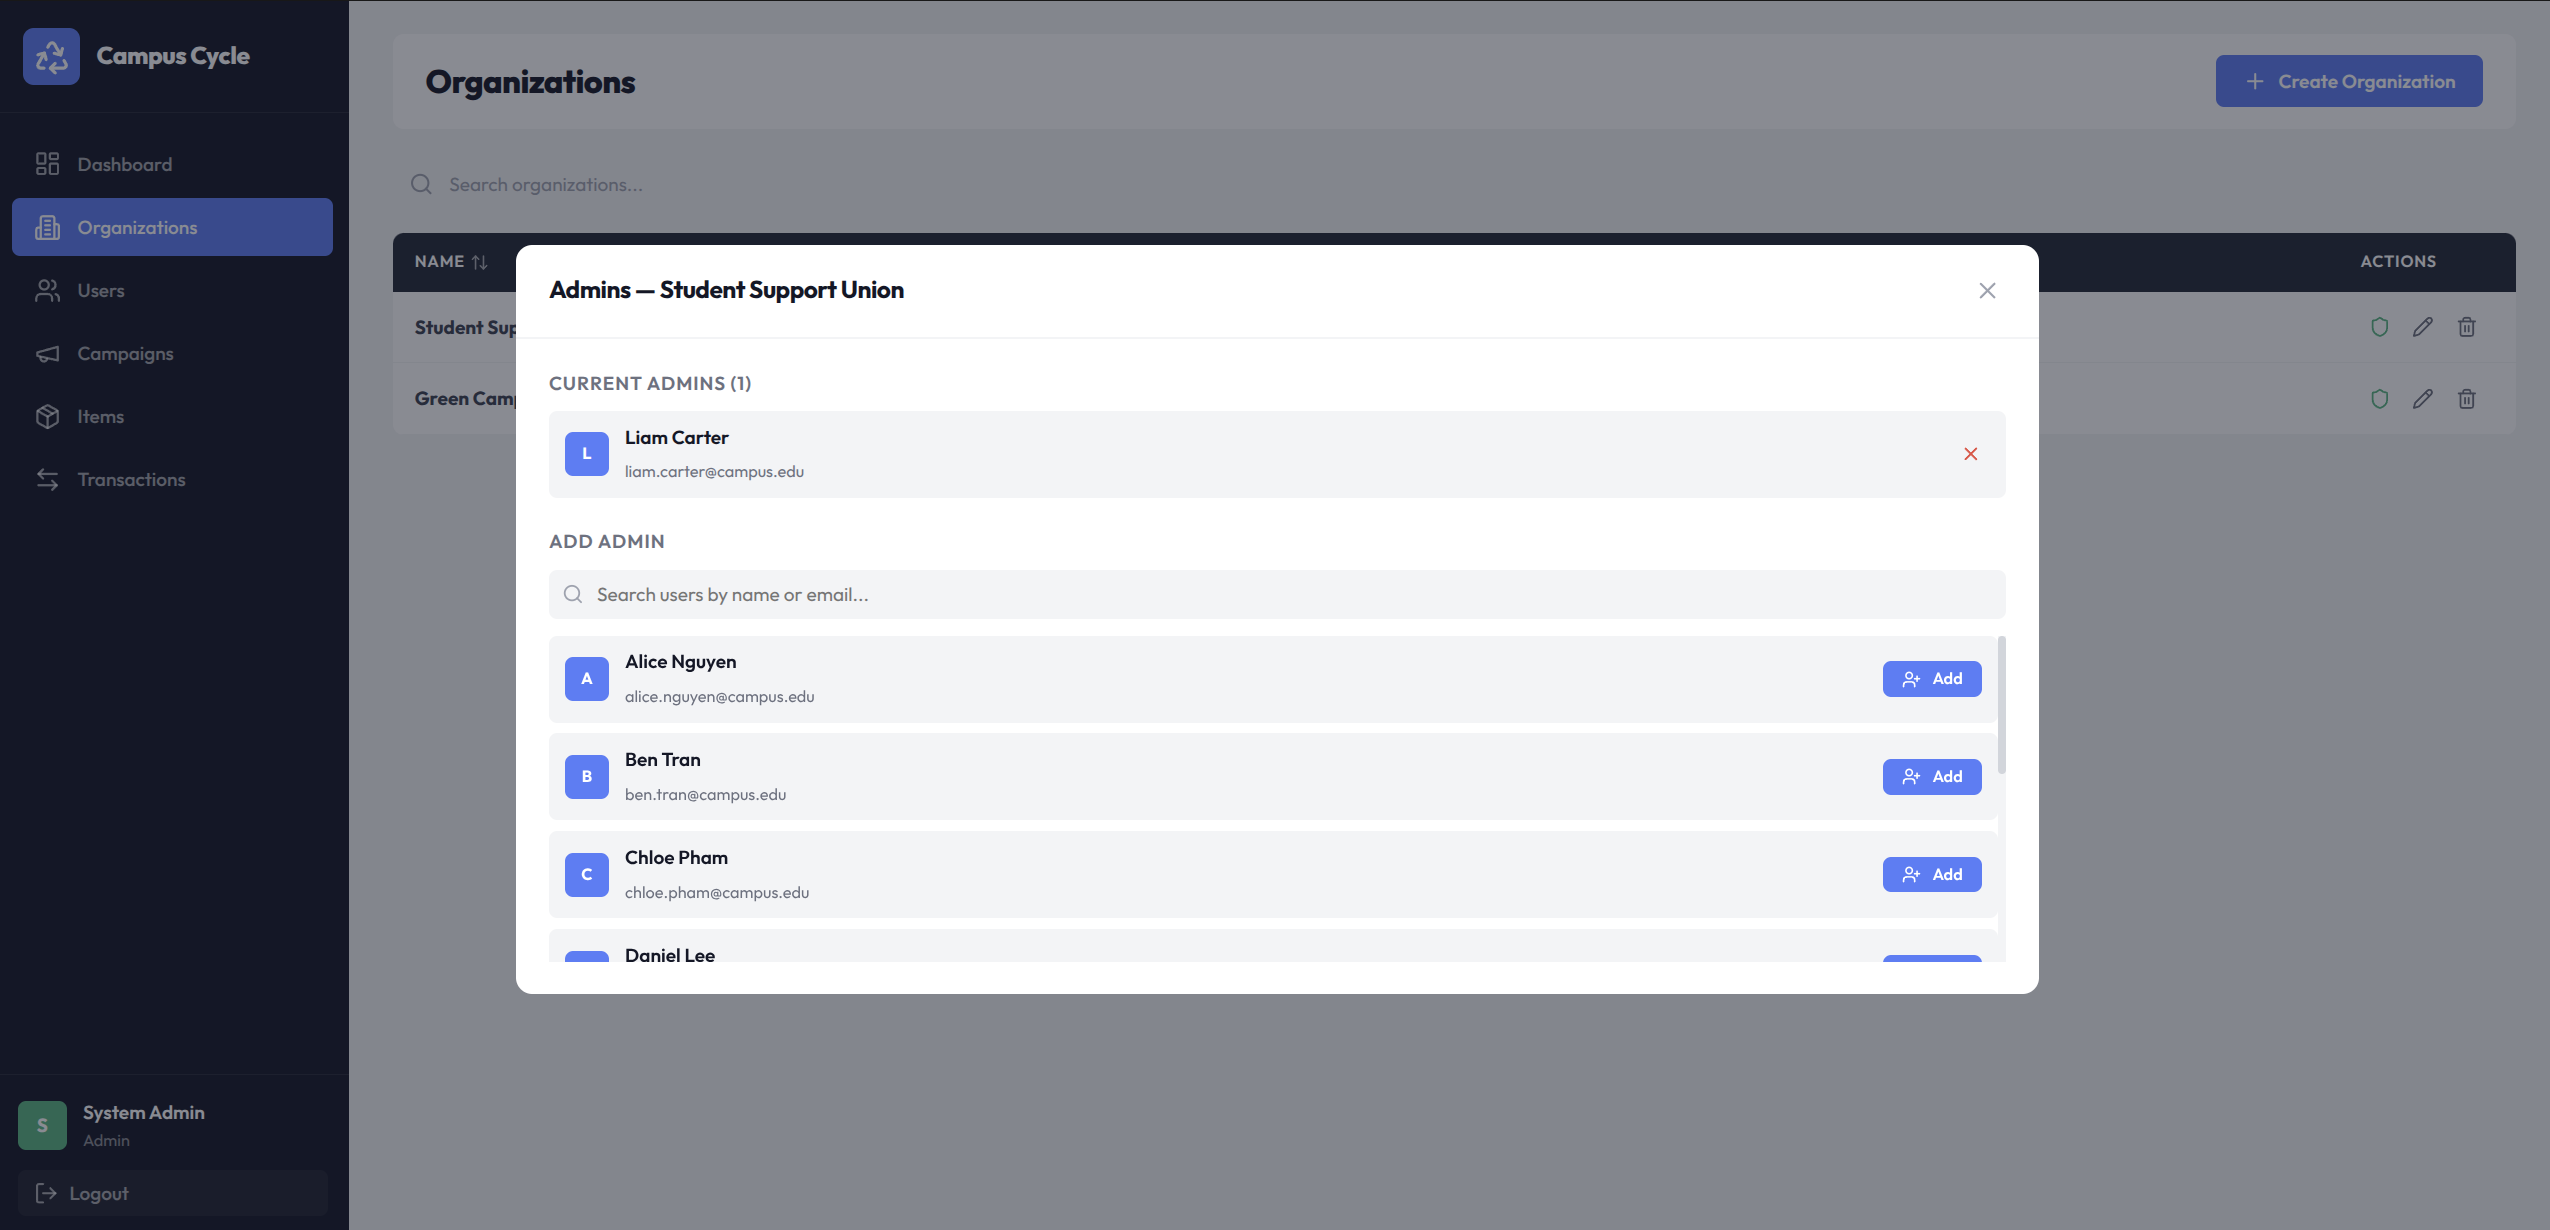
\includegraphics[width=0.75\textwidth]{Organization Approval Modal.png}
    \caption{Organization Admin Management Page}
    \label{fig:organization-admin-management-page}
\end{figure}

Item Management Page: Cho phép system admin kiểm tra và quản lý các items trong hệ thống.

\begin{figure}[H]
\centering
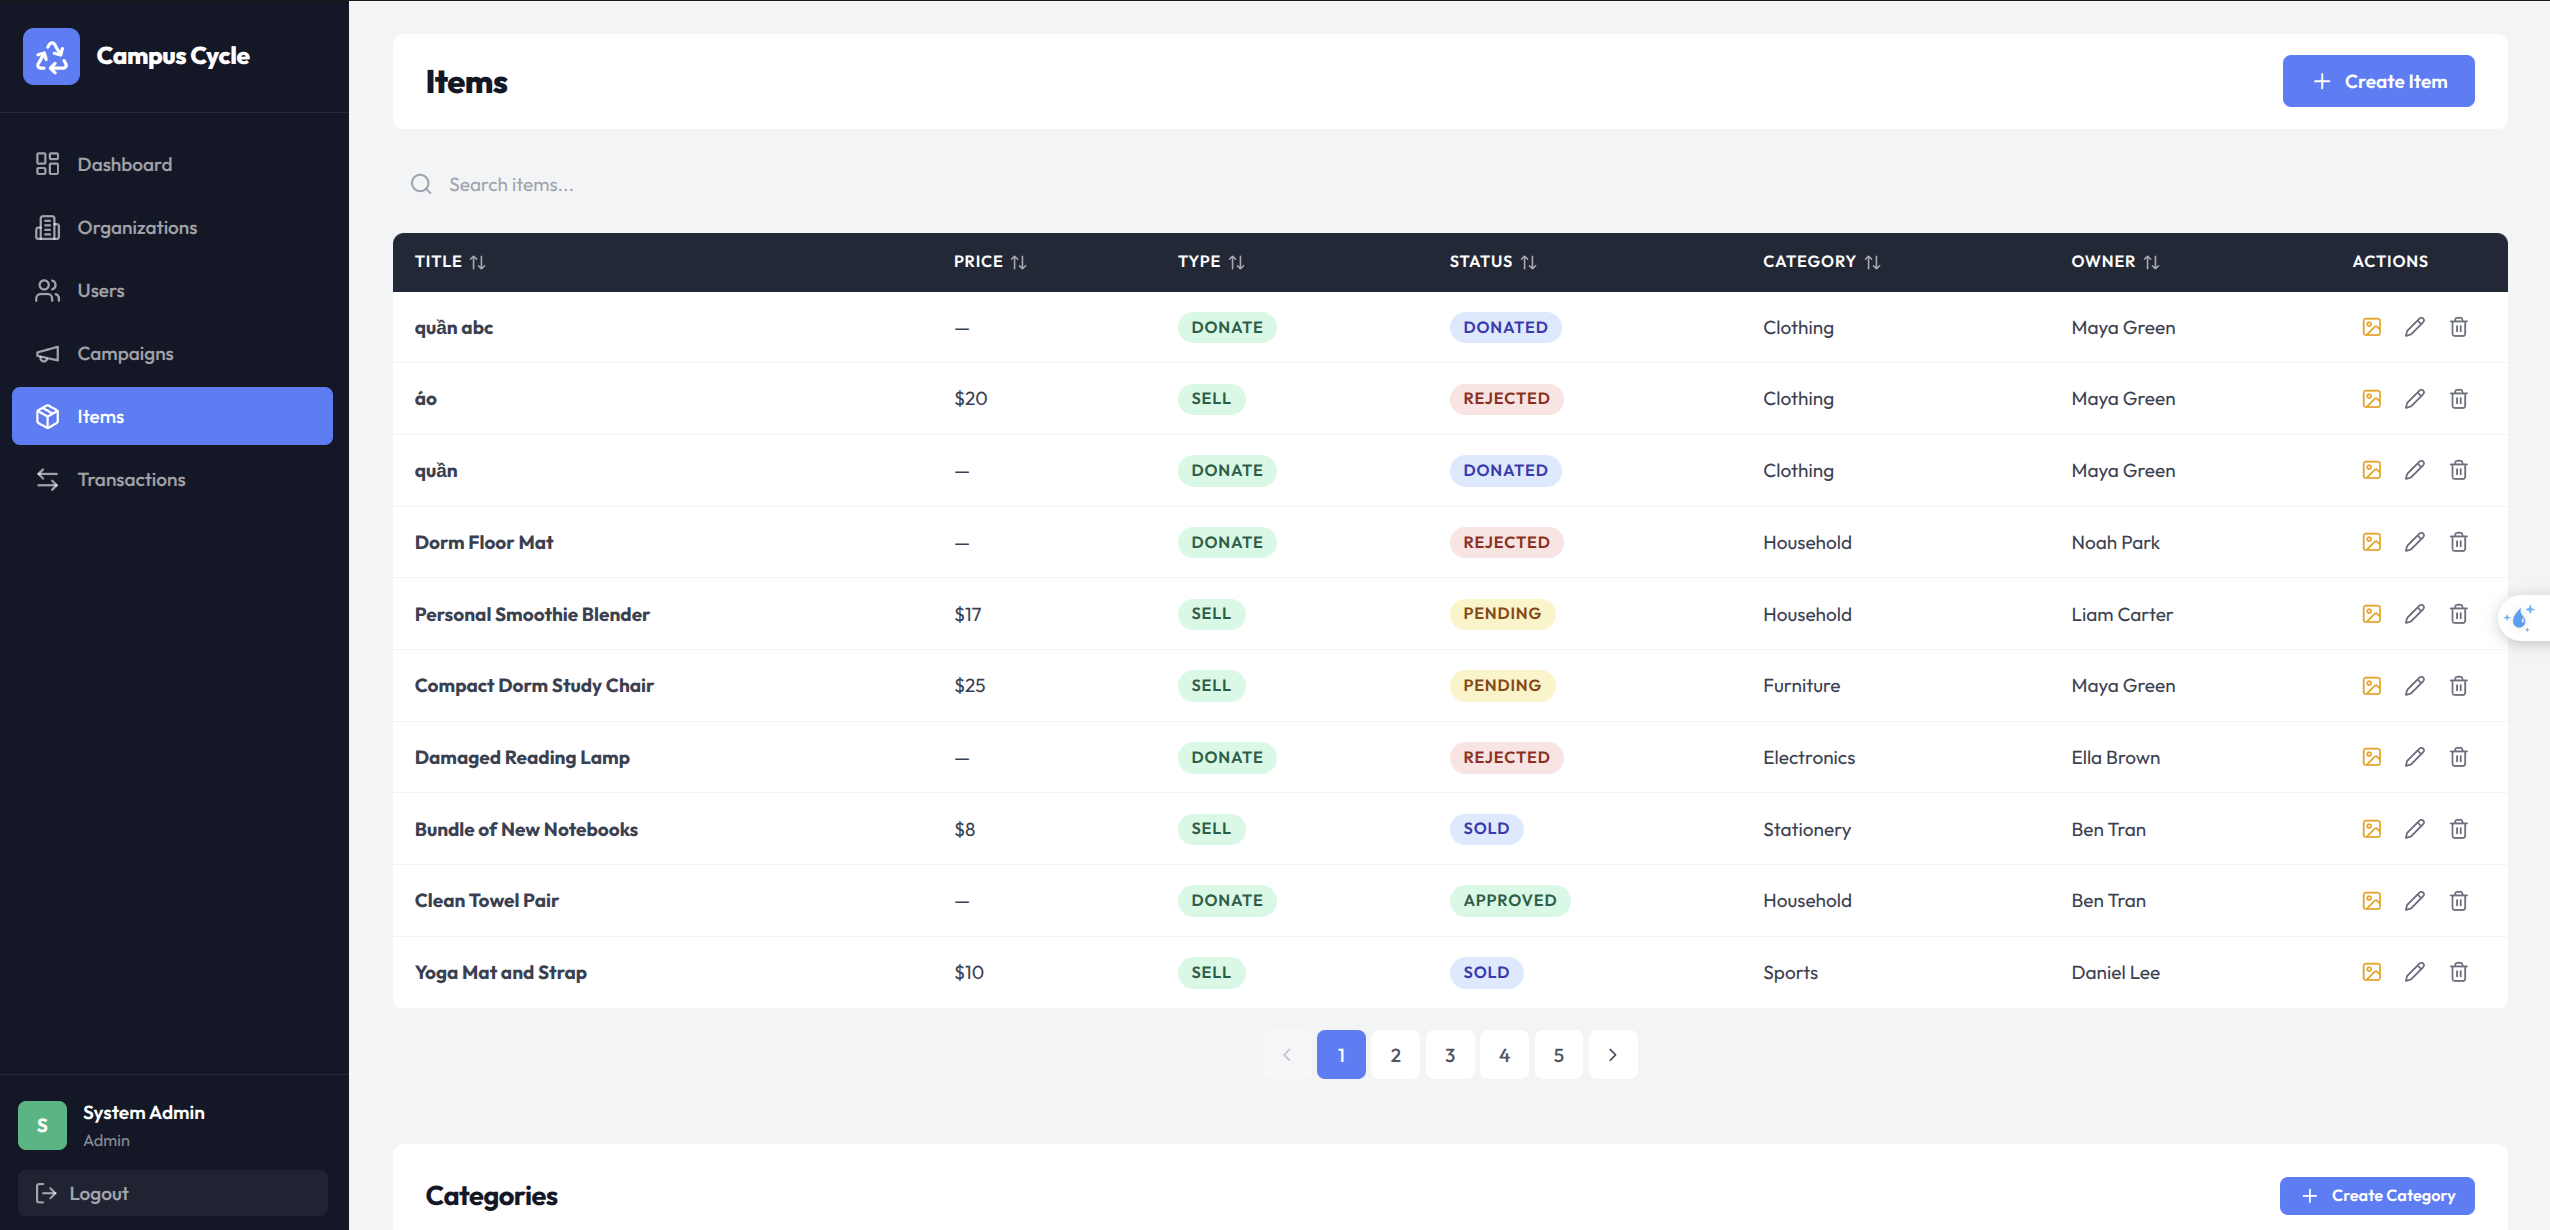
\includegraphics[width=0.75\textwidth]{Item Management Page.png}
\caption{Item Management Page}
\label{fig:item-management-page}
\end{figure}

Category Management Page: Cho phép thêm, sửa, xóa các item categories.

\begin{figure}[H]
\centering
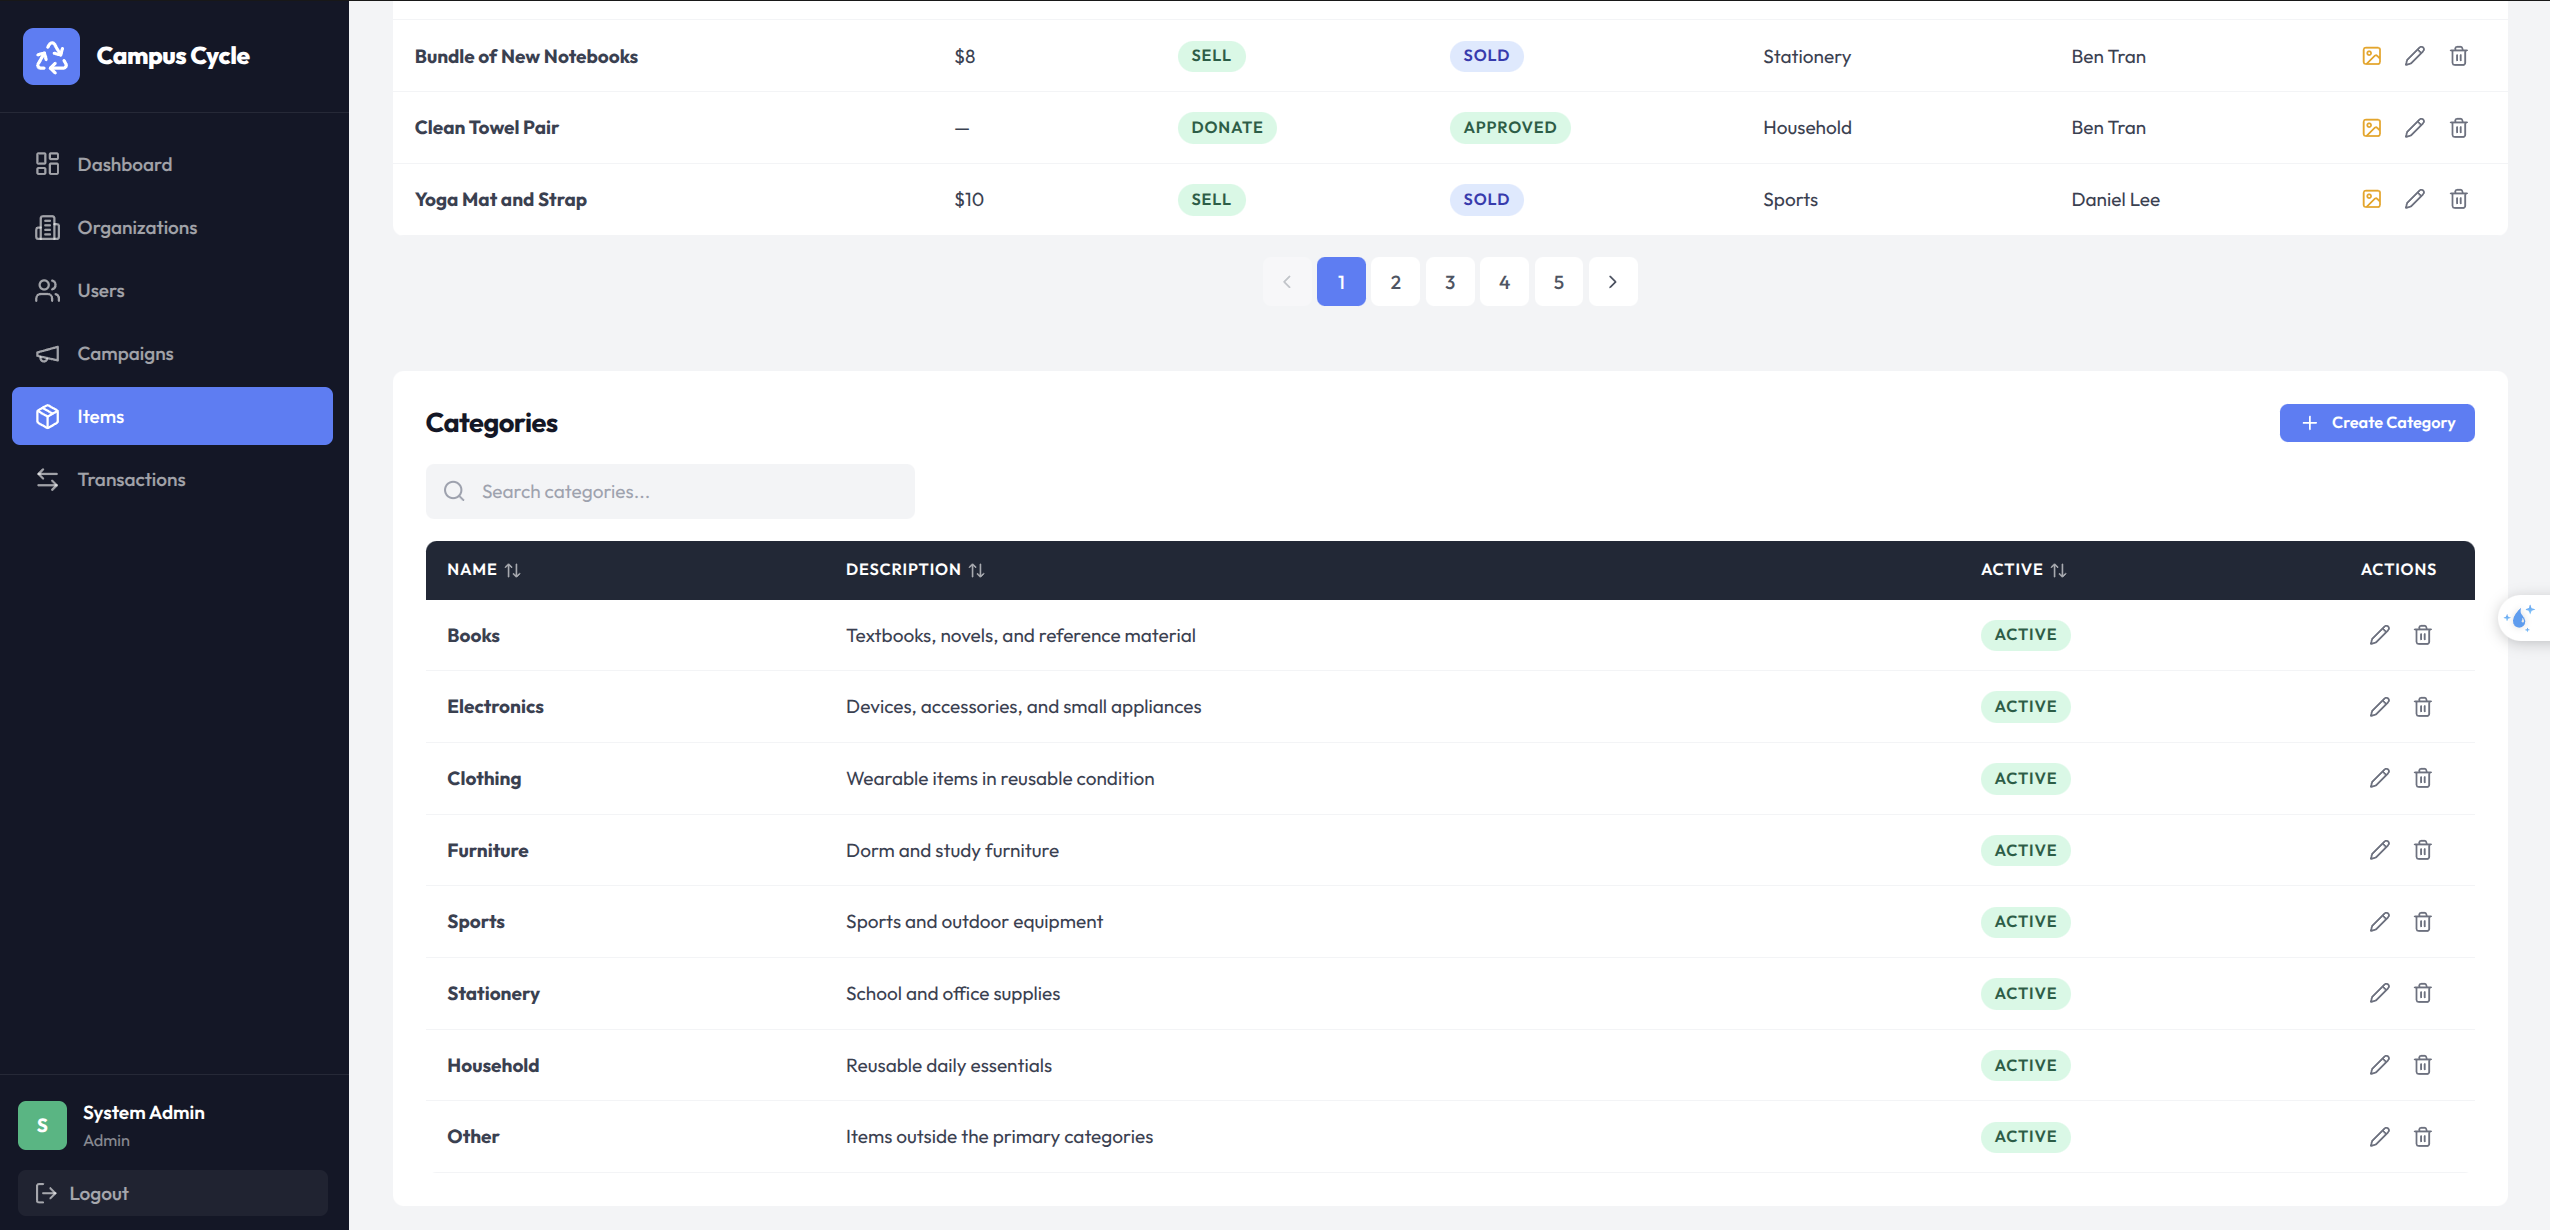
\includegraphics[width=0.75\textwidth]{Category Management Page.png}
\caption{Category Management Page}
\label{fig:category-management-page}
\end{figure}

Transaction Management Page: Theo dõi các transactions mua bán, quyên góp hoặc trạng thái xử lý.

\begin{figure}[H]
\centering
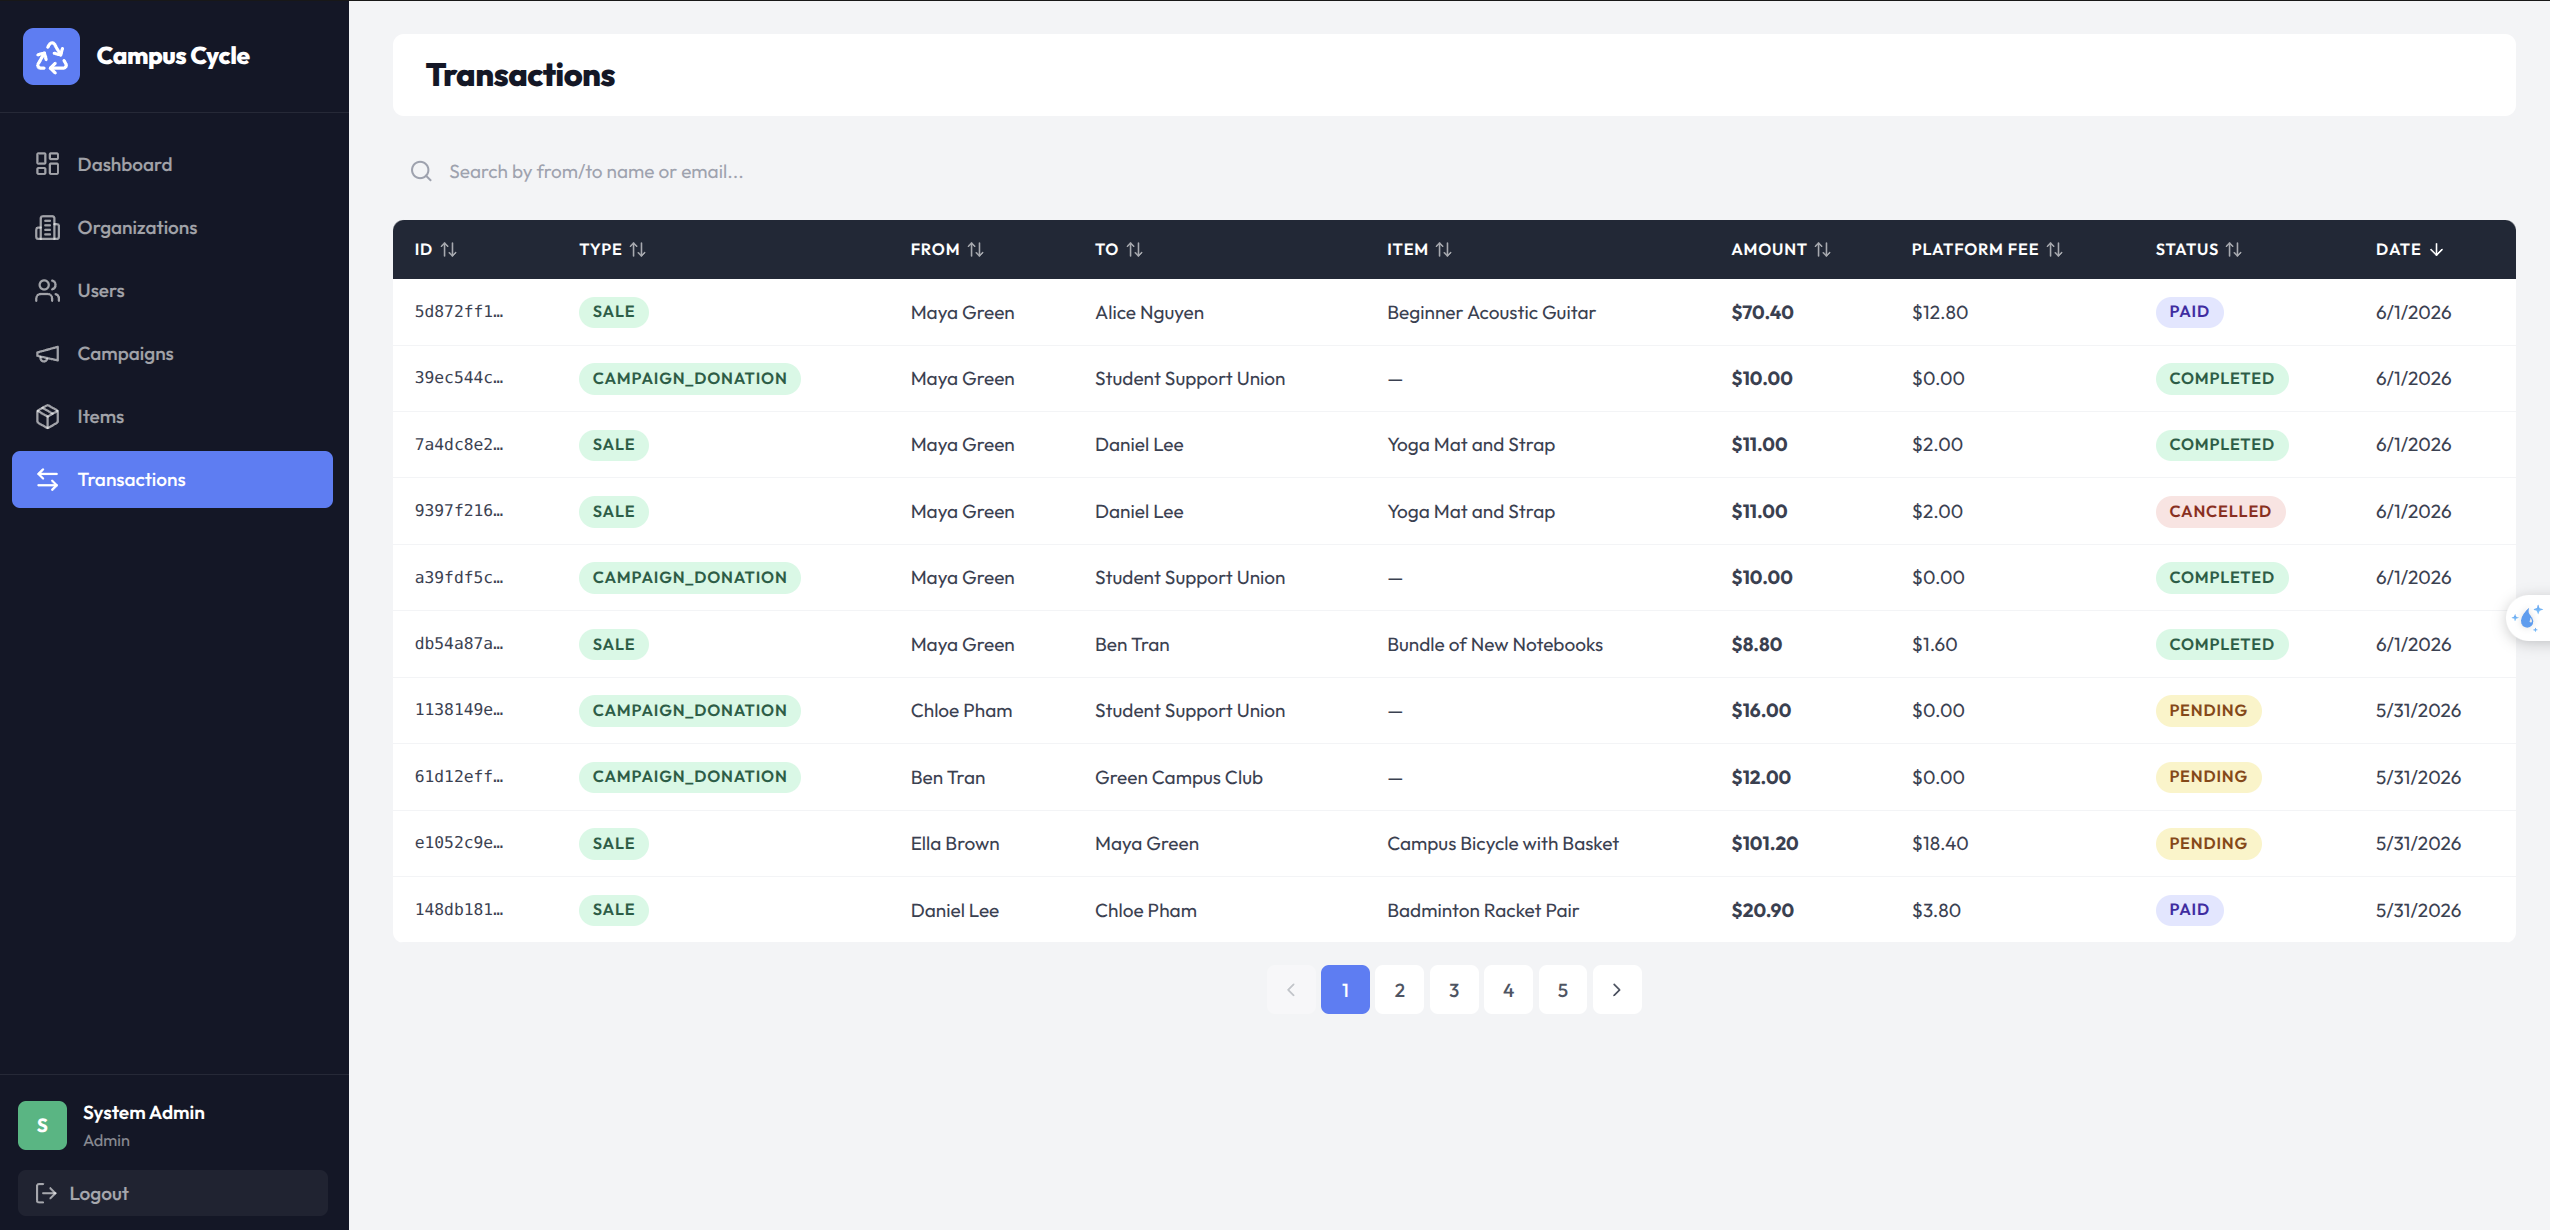
\includegraphics[width=0.75\textwidth]{Transaction Management Page.png}
\caption{Transaction Management Page}
\label{fig:transaction-management-page}
\end{figure}

Campaign Management Page: Theo dõi và quản lý các campaigns.

\begin{figure}[H]
\centering
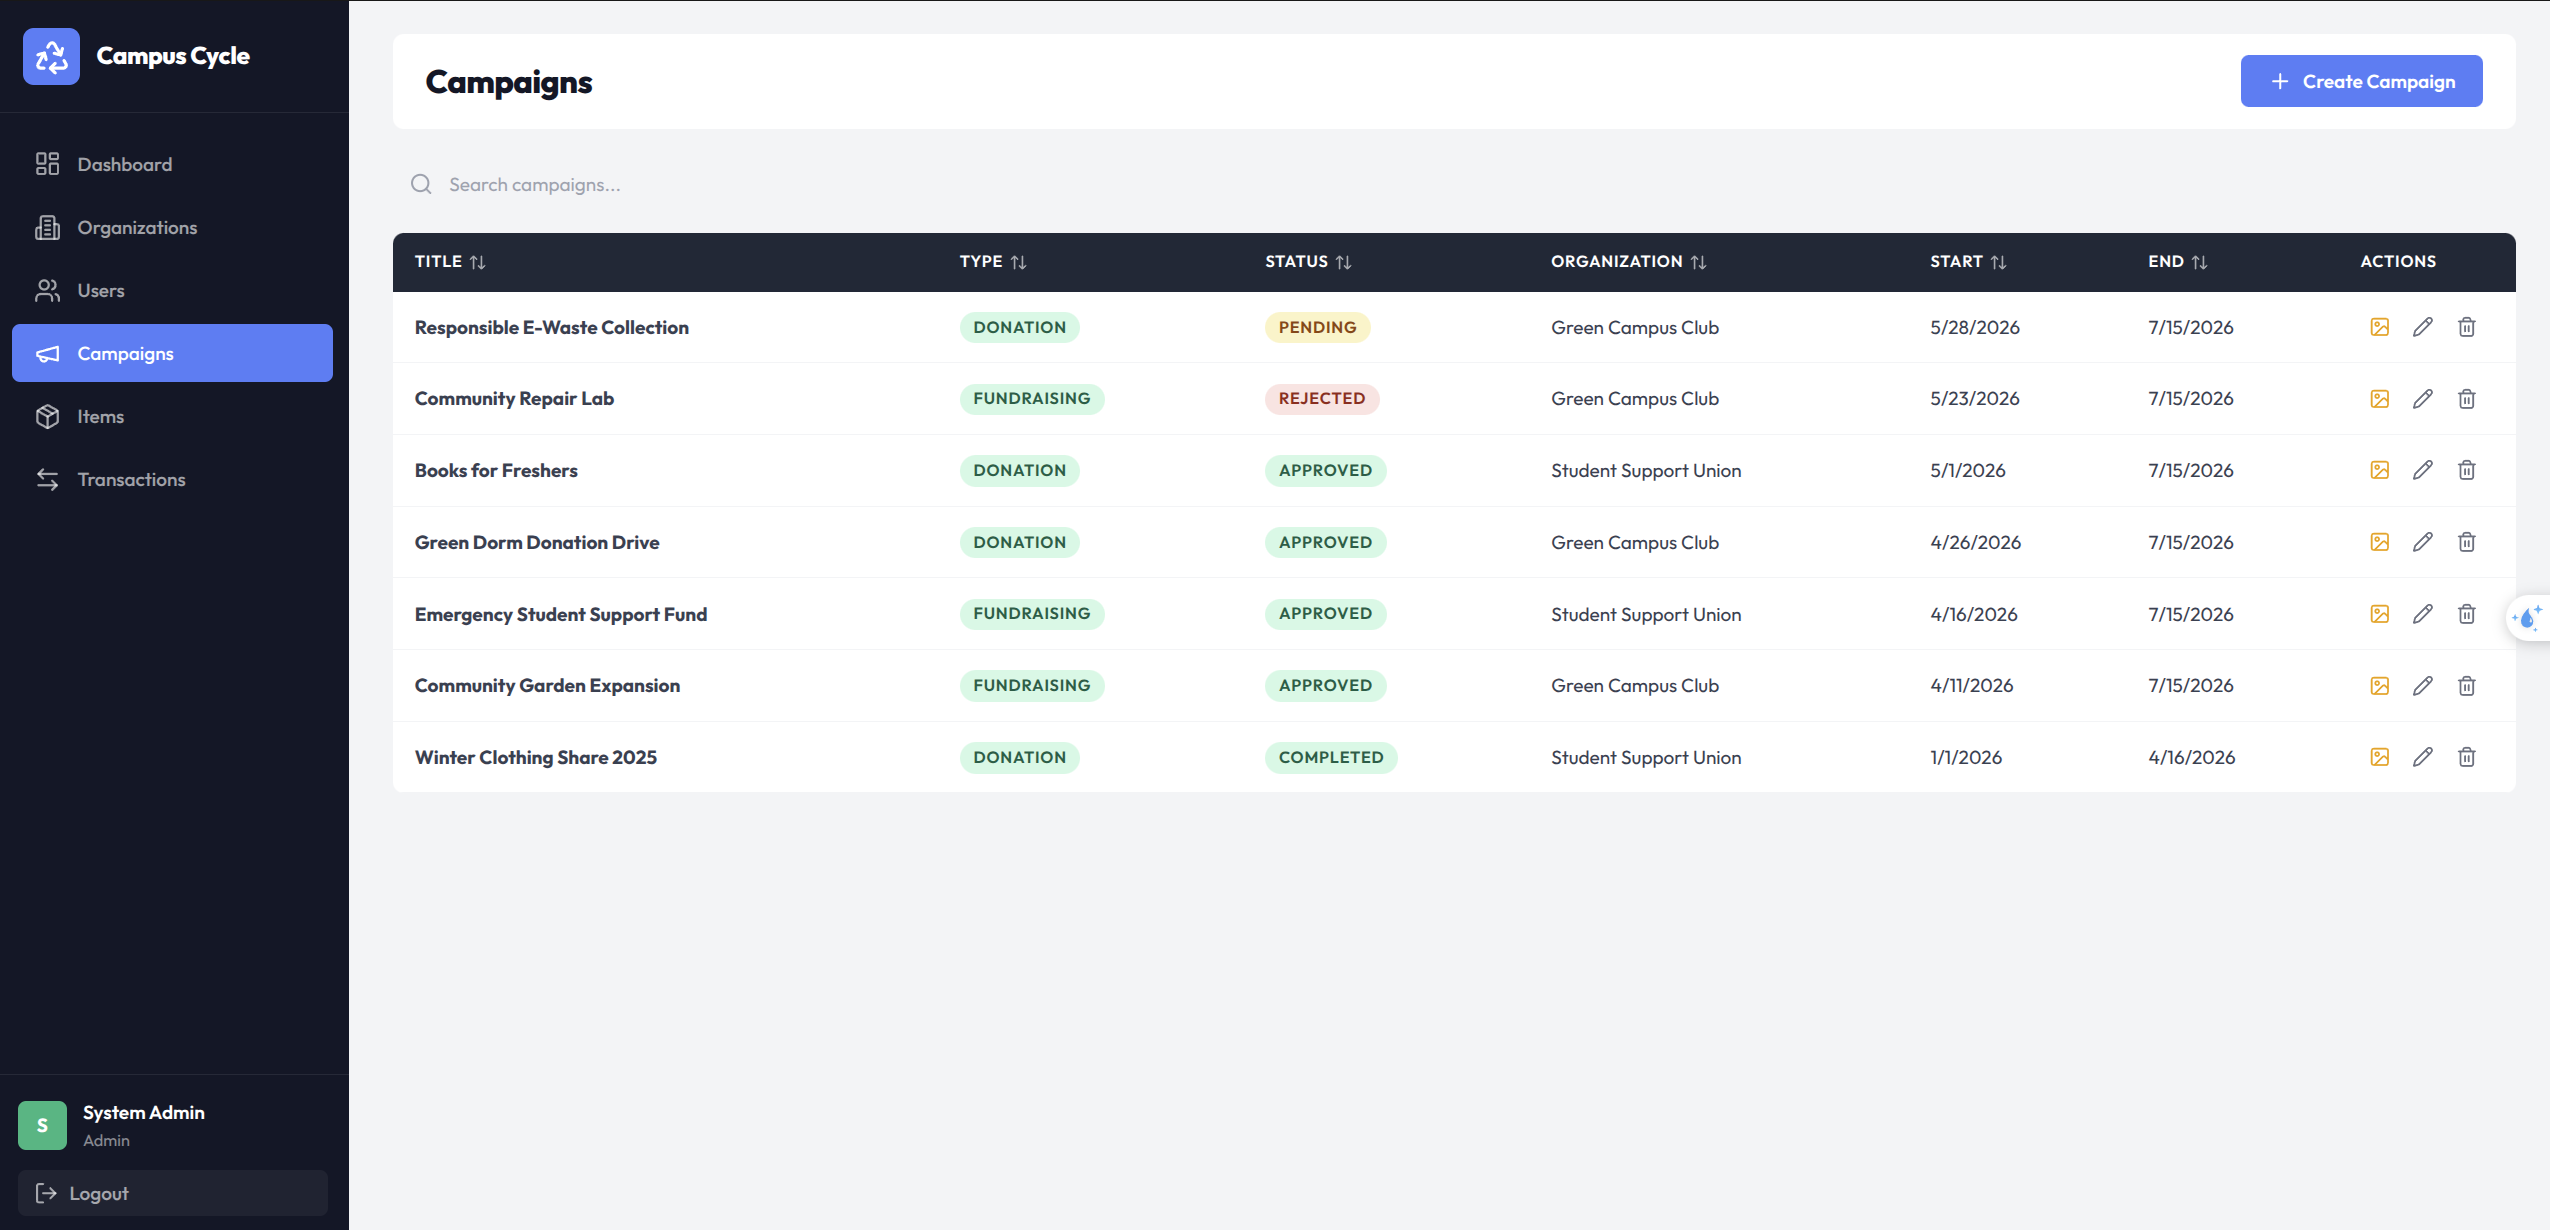
\includegraphics[width=0.75\textwidth]{Campaign Management Page.png}
\caption{Campaign Management Page}
\label{fig:campaign-management-admin-page}
\end{figure}


\chapter{Kết luận và hướng phát triển}

\section{Đánh giá và phân tích}

Sau quá trình khảo sát, phân tích, thiết kế và triển khai hệ thống Campus Cycle Platform, có thể nhận thấy hệ thống đã đáp ứng được mục tiêu cơ bản là xây dựng một nền tảng hỗ trợ thanh lý, quyên góp vật phẩm và gây quỹ trong phạm vi trường học. Thay vì để các hoạt động mua bán hoặc quyên góp diễn ra rời rạc trên nhiều kênh khác nhau như mạng xã hội, biểu mẫu trực tuyến hoặc trao đổi trực tiếp, hệ thống đã tập trung các chức năng này vào một nền tảng thống nhất. Điều này giúp quá trình quản lý trở nên rõ ràng hơn, đồng thời tạo điều kiện để học sinh, giáo viên và các tổ chức trong trường có thể kết nối với nhau một cách thuận tiện và đáng tin cậy hơn.

Một điểm mạnh đáng chú ý của hệ thống là khả năng xây dựng cộng đồng nội bộ có tính tin cậy cao. Campus Cycle Platform được thiết kế dành riêng cho môi trường trường học, nơi các thành viên có mối liên hệ nhất định với nhau thông qua nhà trường. Nhờ đó, các hoạt động giao dịch, quyên góp hoặc tham gia chiến dịch không diễn ra trong một môi trường mở hoàn toàn như các sàn thương mại điện tử thông thường, mà được giới hạn trong một cộng đồng có kiểm soát. Điều này giúp tăng mức độ an toàn cho người dùng, đồng thời làm giảm rủi ro phát sinh từ các giao dịch với người lạ bên ngoài hệ thống.

Bên cạnh đó, hệ thống còn có ưu điểm trong việc kết hợp nhiều hoạt động khác nhau trên cùng một nền tảng. Người dùng không chỉ có thể đăng bán hoặc mua lại các vật phẩm cũ, mà còn có thể quyên góp vật phẩm cho các chiến dịch phù hợp hoặc quyên góp tiền cho các campaign gây quỹ. Việc tích hợp các chức năng thanh lý, quyên góp và gây quỹ trong cùng một hệ thống giúp tối ưu hóa nguồn tài nguyên còn dư thừa trong trường học. Những vật phẩm không còn cần thiết đối với người này vẫn có thể tiếp tục được sử dụng bởi người khác hoặc được chuyển đến các chiến dịch thiện nguyện có nhu cầu.

Ngoài ra, hệ thống có cơ chế kiểm duyệt nội dung và quản lý trạng thái tương đối rõ ràng. Các item và campaign trước khi được công khai cần trải qua quá trình xem xét bởi quản trị viên có thẩm quyền. Cơ chế này giúp hạn chế các bài đăng không phù hợp, giảm nguy cơ xuất hiện thông tin sai lệch và góp phần đảm bảo môi trường sử dụng an toàn cho học sinh, giáo viên. Đối với các vật phẩm quyên góp, Organization Admin cũng có thể theo dõi và cập nhật trạng thái xử lý, từ đó giúp quá trình tiếp nhận và quản lý donated items trở nên minh bạch hơn.

Một ưu điểm khác của Campus Cycle Platform là khả năng hỗ trợ quản lý campaign và transaction một cách có hệ thống. Thay vì phải sử dụng bảng tính hoặc ghi chép thủ công, các tổ chức có thể theo dõi thông tin chiến dịch, số lượng vật phẩm được quyên góp, số tiền nhận được và các dữ liệu thống kê liên quan ngay trong hệ thống. System Admin cũng có thể quan sát tổng quan hoạt động của toàn bộ nền tảng thông qua dashboard và các trang quản lý. Nhờ đó, việc quản lý dữ liệu trở nên nhất quán hơn, giảm sai sót trong quá trình tổng hợp và hỗ trợ tốt hơn cho công tác báo cáo.

Tuy nhiên, bên cạnh các điểm mạnh, hệ thống vẫn còn tồn tại một số hạn chế nhất định. Trước hết, quá trình kiểm duyệt hiện tại vẫn phụ thuộc khá nhiều vào quản trị viên. Khi số lượng item, campaign hoặc donated item tăng lên, System Admin và Organization Admin có thể phải xử lý một lượng lớn dữ liệu trong thời gian ngắn. Điều này có thể gây quá tải, làm chậm quá trình phê duyệt và ảnh hưởng đến trải nghiệm của người dùng. Vì vậy, trong tương lai, hệ thống cần có thêm các cơ chế hỗ trợ tự động nhằm giảm bớt khối lượng công việc thủ công cho quản trị viên.

Một hạn chế khác là hệ thống chưa thể kiểm soát hoàn toàn chất lượng thực tế của vật phẩm được đăng tải. Các thông tin như hình ảnh, mô tả, tình trạng sử dụng hoặc giá trị của sản phẩm chủ yếu dựa trên dữ liệu do người dùng cung cấp. Hệ thống có thể kiểm duyệt nội dung bài đăng ở mức thông tin, nhưng chưa thể xác minh chính xác chất lượng vật phẩm ngoài thực tế. Điều này có thể dẫn đến trường hợp sản phẩm nhận được không hoàn toàn giống với mô tả ban đầu, đặc biệt trong các giao dịch mua bán giữa các thành viên.

Ngoài ra, hệ thống hiện chưa hỗ trợ đầy đủ các chức năng giao tiếp trực tiếp giữa người mua và người bán, hoặc giữa member và organization admin. Trong nhiều trường hợp, các bên vẫn cần sử dụng kênh liên lạc bên ngoài để trao đổi thêm về thời gian giao nhận, địa điểm gặp mặt hoặc các thông tin chi tiết khác. Việc thiếu chức năng chat nội bộ có thể làm giảm tính liền mạch của quy trình giao dịch. Đây là một điểm cần được bổ sung trong các phiên bản phát triển tiếp theo để người dùng có thể thực hiện toàn bộ quá trình trao đổi ngay trong hệ thống.

\section{Kết luận}

Campus Cycle Platform là một hệ thống được xây dựng nhằm hỗ trợ các hoạt động trao đổi, thanh lý, quyên góp vật phẩm và gây quỹ trong môi trường trường học. Hệ thống xuất phát từ nhu cầu thực tế về việc tái sử dụng các vật phẩm còn giá trị, giảm lãng phí tài nguyên và tạo ra một kênh kết nối đáng tin cậy giữa học sinh, giáo viên và các tổ chức trong trường. Thông qua nền tảng này, các vật phẩm như sách vở, đồng phục, đồ dùng học tập, thiết bị điện tử hoặc các vật dụng cá nhân khác có thể được tiếp tục sử dụng thay vì bị bỏ không hoặc thải bỏ.

Về mặt chức năng, hệ thống đã hỗ trợ các nghiệp vụ chính như đăng ký, đăng nhập, quản lý thông tin cá nhân, đăng tải item, xem danh sách item, xem chi tiết item, gửi yêu cầu mua hàng, quyên góp vật phẩm, quyên góp tiền cho campaign và theo dõi trạng thái giao dịch. Đối với nhóm quản trị, hệ thống cung cấp các chức năng quản lý user, organization, category, item, transaction và campaign. Đối với Organization Admin, hệ thống hỗ trợ việc tạo và quản lý campaign, theo dõi donated items, kiểm duyệt vật phẩm quyên góp và xem thống kê liên quan đến chiến dịch. Các chức năng này tạo thành một quy trình tương đối đầy đủ, phục vụ cho cả người dùng thông thường và các nhóm quản trị trong hệ thống.

Về mặt quản lý, Campus Cycle Platform góp phần thay thế các phương thức quản lý thủ công trước đây bằng một hệ thống tập trung và có cấu trúc. Các dữ liệu về item, campaign, donation, transaction và user được lưu trữ trong cơ sở dữ liệu, giúp việc truy xuất và thống kê trở nên thuận tiện hơn. Việc có các dashboard và trang quản lý riêng cho từng nhóm người dùng cũng giúp quá trình vận hành hệ thống rõ ràng hơn. Nhờ đó, nhà trường hoặc các tổ chức có thể dễ dàng theo dõi hiệu quả của các hoạt động mua bán, gây quỹ và quyên góp.

Bên cạnh giá trị về mặt chức năng, hệ thống còn mang ý nghĩa xã hội trong môi trường học đường. Campus Cycle Platform khuyến khích tinh thần chia sẻ, tiết kiệm và hỗ trợ lẫn nhau giữa các thành viên trong trường. Những vật phẩm không còn phù hợp với nhu cầu của một người vẫn có thể trở thành tài nguyên hữu ích đối với người khác. Đồng thời, các campaign quyên góp và gây quỹ cũng giúp kết nối cộng đồng, hỗ trợ các hoạt động thiện nguyện và tạo ra môi trường học tập có trách nhiệm hơn với xã hội và môi trường.

Nhìn chung, hệ thống đã đáp ứng được các mục tiêu ban đầu của đề tài là xây dựng một nền tảng nội bộ hỗ trợ thanh lý, quyên góp và quản lý chiến dịch trong trường học. Mặc dù vẫn còn một số hạn chế về kiểm soát chất lượng sản phẩm, khả năng tự động hóa kiểm duyệt và chức năng giao tiếp nội bộ, Campus Cycle Platform vẫn là một giải pháp có tính ứng dụng thực tế. Nếu tiếp tục được hoàn thiện và mở rộng, hệ thống có thể trở thành một công cụ hữu ích trong việc thúc đẩy tái sử dụng tài nguyên và nâng cao hiệu quả quản lý các hoạt động cộng đồng trong nhà trường.

\section{Hướng phát triển}

Trong tương lai, Campus Cycle Platform có thể được phát triển theo nhiều hướng nhằm nâng cao tính tiện dụng, độ an toàn và khả năng mở rộng của hệ thống. Trước hết, hệ thống nên được tích hợp với email nội bộ của trường. Việc sử dụng email do nhà trường cấp có thể giúp xác thực người dùng chính xác hơn, đảm bảo chỉ những học sinh, giáo viên hoặc nhân sự thuộc trường mới được phép tham gia hệ thống. Ngoài ra, email cũng có thể được sử dụng để gửi thông báo về trạng thái bài đăng, kết quả kiểm duyệt, thông tin giao dịch, cập nhật campaign hoặc nhắc nhở người dùng khi có hành động cần xử lý.

Một hướng phát triển quan trọng khác là ứng dụng trí tuệ nhân tạo để hỗ trợ quản trị viên trong quá trình kiểm duyệt và phân loại dữ liệu. AI có thể được sử dụng để phát hiện nội dung không phù hợp trong mô tả sản phẩm, nhận diện hình ảnh vi phạm quy định hoặc gợi ý danh mục phù hợp cho item được đăng tải. Đối với các campaign quyên góp, AI cũng có thể hỗ trợ đề xuất campaign phù hợp với loại vật phẩm mà người dùng muốn quyên góp. Điều này không chỉ giúp tăng trải nghiệm người dùng mà còn giảm khối lượng công việc thủ công cho System Admin và Organization Admin.

Hệ thống cũng nên bổ sung chức năng chat nội bộ để hỗ trợ quá trình trao đổi giữa các bên. Khi người mua quan tâm đến một item, họ có thể nhắn tin trực tiếp cho người bán để hỏi thêm thông tin hoặc thống nhất thời gian, địa điểm giao nhận. Tương tự, member có thể trao đổi với Organization Admin khi muốn quyên góp vật phẩm cho campaign. Việc bổ sung chức năng chat sẽ giúp toàn bộ quá trình giao tiếp diễn ra ngay trong hệ thống, hạn chế việc phải chuyển sang các nền tảng bên ngoài và giúp lịch sử trao đổi được lưu lại rõ ràng hơn.

Bên cạnh chat nội bộ, chức năng đánh giá sau giao dịch cũng là một hướng phát triển cần thiết. Sau khi một giao dịch mua bán hoặc quyên góp hoàn tất, người dùng có thể đánh giá mức độ hài lòng, chất lượng vật phẩm và thái độ hợp tác của bên còn lại. Các đánh giá này sẽ góp phần xây dựng mức độ uy tín cho từng tài khoản trong hệ thống. Khi người dùng có lịch sử giao dịch tốt và nhận được đánh giá tích cực, các thành viên khác sẽ có thêm cơ sở để tin tưởng khi thực hiện giao dịch.

Ngoài phiên bản web, hệ thống có thể được phát triển thêm ứng dụng di động trên Android và iOS. Trong thực tế, học sinh và giáo viên thường sử dụng điện thoại thông minh để truy cập thông tin hằng ngày. Vì vậy, việc có mobile application sẽ giúp người dùng dễ dàng đăng item, chụp ảnh vật phẩm, theo dõi campaign, nhận thông báo và phản hồi nhanh hơn. Ứng dụng di động cũng có thể tích hợp push notification để thông báo tức thời khi item được duyệt, có người gửi yêu cầu mua hàng hoặc campaign có cập nhật mới.

Trong dài hạn, Campus Cycle Platform có thể được mở rộng để phục vụ nhiều trường học khác nhau thay vì chỉ giới hạn trong một trường. Khi đó, hệ thống cần hỗ trợ mô hình multi-school, trong đó mỗi trường có không gian dữ liệu, danh sách user, organization và campaign riêng. Việc mở rộng này sẽ giúp hệ thống có khả năng ứng dụng rộng hơn, đồng thời tạo ra mạng lưới mua bán và quyên góp giữa nhiều cộng đồng học đường. Tuy nhiên, để thực hiện được điều này, hệ thống cần tiếp tục được tối ưu về hiệu năng, bảo mật, phân quyền và khả năng quản lý dữ liệu.

Tóm lại, hướng phát triển của Campus Cycle Platform không chỉ tập trung vào việc bổ sung chức năng mới, mà còn hướng đến việc nâng cao chất lượng vận hành, tăng tính tự động hóa và cải thiện trải nghiệm người dùng. Các chức năng như xác thực bằng email trường, AI hỗ trợ kiểm duyệt, chat nội bộ, đánh giá sau giao dịch và ứng dụng di động sẽ giúp hệ thống trở nên hoàn thiện hơn. Khi được phát triển đầy đủ, Campus Cycle Platform có thể trở thành một nền tảng hữu ích trong việc xây dựng cộng đồng học đường bền vững, tiết kiệm tài nguyên và thúc đẩy tinh thần chia sẻ trong trường học.


\clearpage
\chapter*{Tài liệu tham khảo}
\addcontentsline{toc}{chapter}{Tài liệu tham khảo}

\textbf{Tài liệu tham khảo}

\begin{enumerate}[label={[\arabic*]}, leftmargin=1.5cm]

\item Joseph Valacich, Joey George, \textit{Modern Systems Analysis and Design}, 8th Edition, Pearson Education, 2019.

\item Dư Phương Hạnh, \textit{Slide bài giảng môn Phân tích và Thiết kế các Hệ thống Thông tin}, Trường Đại học Công nghệ - Đại học Quốc gia Hà Nội, 2026.

\end{enumerate}

\end{document}
